% Desenvolvido por: Prof. Dr. David Buzatto
%
% Baseado na documentação do abntex2 e nos modelos em
% Microsoft Word propostos pela Profa. Dra. Rosana F. L. Rodrigues
% e pela bibliotecária M.Sc. Maria Carolina Gonçalves do Câmpus
% São João da Boa Vista do IFSP.
%
% Versão 1.51
% Data: 06/11/2018
%
% Adequação ao Modelo do Câmpus Birigui
% Realizado por Helen de Freitas Santos e Adrano de Souza Marques
% Data: 27/11/2020

\documentclass[
	% -- opções da classe memoir --
	12pt,				% tamanho da fonte
	openany,			% openright = capítulos começam em pág ímpar (insere página vazia caso preciso)
	oneside,			% twoside para impressão em verso e anverso. Oposto a oneside
	a4paper,			% tamanho do papel. 
	%normalfigtabnum,
	%pnumromarab,
	% -- opções da classe abntex2 --
	chapter=TITLE,		% títulos de capítulos convertidos em letras maiúsculas
	%section=TITLE,		% títulos de seções convertidos em letras maiúsculas
	%subsection=TITLE,	% títulos de subseções convertidos em letras maiúsculas
	%subsubsection=TITLE,% títulos de subsubseções convertidos em letras maiúsculas
	% -- opções do pacote babel --
	english,			% idioma adicional para hifenização
	french,				% idioma adicional para hifenização
	spanish,			% idioma adicional para hifenização
	brazil,				% o último idioma é o principal do documento
]{abntex2}






% ---------------------------------------------------------------------------------
%                                   PACOTES
% ---------------------------------------------------------------------------------

% ---
% Pacotes básicos 
% ---
\usepackage{lmodern}			% Usa a fonte Latin Modern			
\usepackage[T1]{fontenc}		% Selecao de codigos de fonte.
\usepackage[utf8]{inputenc}		% Codificacao do documento (conversão automática dos acentos)
\usepackage{lastpage}			% Usado pela Ficha catalográfica
\usepackage{indentfirst}		% Indenta o primeiro parágrafo de cada seção.
\usepackage{xcolor,colortbl}	% Controle das cores
\usepackage{graphicx}			% Inclusão de gráficos
\usepackage{microtype} 			% para melhorias de justificação
\usepackage{hyperref}
\usepackage{subfig}
\usepackage{epigraph}
\usepackage{url}
\usepackage{placeins}
\usepackage{multirow}
\usepackage[figuresright]{rotating}
\usepackage{chemfig}
\usepackage{amsmath}
\usepackage{amssymb}
\usepackage{enumitem}
\usepackage{bigints}
\usepackage{listings}
\usepackage{etoolbox}
\usepackage[final]{pdfpages}
\usepackage{bigstrut}
\usepackage{longtable}
\usepackage{algpseudocode}
\usepackage{placeins}   % \FloatBarrier
\usepackage{enumitem}   % enumerate com nosep
\usepackage{longtable}  % tabelas longas (não usado aqui, mas útil)
% ---

% ---
% Pacotes adicionais, usados apenas no âmbito do Modelo Canônico do abnteX2
% ---
\usepackage{lipsum}				% para geração de dummy text
% ---

% ---
% Pacotes de citações
% ---
\usepackage{csquotes}
\usepackage[style=abnt, backref=true, backend=biber]{biblatex}
\addbibresource{referencias.bib}


% ---------------------------------------------------------------------------------
%                          CONFIGURAÇÕES DOS PACOTES
% ---------------------------------------------------------------------------------


% listagens
\definecolor{corComentario}{RGB}{150,150,150}
\definecolor{corString}{RGB}{206,123,0}
\definecolor{corPalavraChave}{RGB}{0,0,230}

\lstset{
	numbers=left,
	stepnumber=1,
	firstnumber=1,
	numberstyle=\footnotesize,
	extendedchars=true,
	breaklines=true,
	lineskip=0pt,
	frame=tb,
	basicstyle=\ttfamily\footnotesize,
	showstringspaces=false,
	stringstyle=\color{corString},
	commentstyle=\color{corComentario},
	keywordstyle=\color{corPalavraChave}
}

% ---
% Tradução do Algpseudocode para PT-BR
% ---
\algrenewcommand\algorithmicfunction{\textbf{função}}
\algrenewcommand\algorithmicend{\textbf{fim}}
\algrenewcommand\algorithmicif{\textbf{se}}
\algrenewcommand\algorithmicthen{\textbf{então}}
\algrenewcommand\algorithmicelse{\textbf{senão}}
\algrenewcommand\algorithmicfor{\textbf{para}}
\algrenewcommand\algorithmicforall{\textbf{para cada}}
\algrenewcommand\algorithmicdo{\textbf{faça}}
\algrenewcommand\algorithmicreturn{\textbf{retornar}}

\newcolumntype{Y}{>{\centering\arraybackslash}X}

\newcommand{\ano}[1]{\def \oano {#1}}
\newcommand{\imprimirano}{\oano}

\newcommand{\mes}[1]{\def \omes {#1}}
\newcommand{\imprimirmes}{\omes}

\newcommand{\subtitulo}[1]{\def \osubtitulo {#1}}
\newcommand{\imprimirsubtitulo}{\osubtitulo}

\newcommand{\area}[1]{\def \aarea {#1}}
\newcommand{\imprimirarea}{\aarea}

\renewcommand{\coorientador}[1]{\def \ocoorientador {#1}}
\renewcommand{\imprimircoorientador}{\ocoorientador}

\newcommand{\grau}[1]{\def \ograu {#1}}
\newcommand{\imprimirgrau}{\ograu}

\newcommand{\curso}[1]{\def \ocurso {#1}}
\newcommand{\imprimircurso}{\ocurso}


% ---
% Informações de dados para CAPA e FOLHA DE ROSTO
% ---

\curso{Engenharia da Computação}
\grau{Bacharelado}

%exemplos
%\curso{Tecnologia em Sistemas para Internet}
%\grau{Tecnólogo em Sistemas para Internet}
%\curso{Especialização em Desenvolvimento de Aplicações para Dispositivos Móveis}
%\grau{Especialista em Desenvolvimento de Aplicações para Dispositivos Móveis}

\titulo{Sistema Especialista Educacional para Validação de Compatibilidade de Hardware baseado em Problema de Satisfação de Restrições (CSP).}

% caso não haja subtítulo, comente a linha abaixo
\subtitulo{subtítulo (se houver)}

\tipotrabalho{Trabalho de Conclusão de Curso}
\area{Área de Concentração do Trabalho}

\autor{Henrique José de Souza}
\orientador{Profa. Dra. Helen de Freitas Santos}

% caso não haja coorientador, comente a linha abaixo
%\coorientador{Prof./Profa. Me./Dr./Dra. Nome Completo}

\local{Birigui}
\mes{MÊS}
\ano{2026}

\instituicao{%
	Instituto Federal de Educação, Ciência e Tecnologia de São Paulo
	\par
	Câmpus Birigui
}

\preambulo{\imprimirtipotrabalho\ apresentado ao Instituto Federal de Educação, Ciência e Tecnologia de São Paulo, como requisito parcial para conclusão do curso de \imprimircurso.
\\
\\
Área de Concentração: \imprimirarea}
% ---


% ---
% Configurações de aparência do PDF final
% ---

% alterando o aspecto da cor azul
\definecolor{blue}{RGB}{41,5,195}

% informações do PDF
\makeatletter
\hypersetup{
	%pagebackref=true,
	pdftitle={\@title}, 
	pdfauthor={\@author},
	pdfsubject={\imprimirpreambulo},
	pdfcreator={Nome Completo},
	pdfkeywords={Palavra chave 1}{Palavra chave 2}{Palavra chave 3}{Palavra chave n}, 
	colorlinks=true,       		% false: boxed links; true: colored links
	linkcolor=black,          	% color of internal links
	citecolor=black,       		% color of links to bibliography
	filecolor=black,      		% color of file links
	urlcolor=black,
	bookmarksdepth=4
}
\makeatother
% --- 


% ---
% Comandos do autor
% ---

% comando para inserir autor e ano
\newcommand{\citeauthorandyear}[1]{\citeauthoronline{#1} (\citeyear{#1})}


% ---
% Novo list of (listings) para Quadros
% ---

\newcommand{\quadroname}{Quadro}
\newcommand{\listofquadrosname}{Lista de Quadros}

\newfloat[chapter]{quadro}{loq}{\quadroname}
\newlistof{listofquadros}{loq}{\listofquadrosname}
\newlistentry{quadro}{loq}{0}

% configurações para atender às regras da ABNT
\setfloatadjustment{quadro}{\centering}
\counterwithout{quadro}{chapter}
\renewcommand{\cftquadroname}{\quadroname\space} 
\renewcommand*{\cftquadroaftersnum}{\hfill--\hfill}

% Configuração de posicionamento padrão:
\setfloatlocations{quadro}{hbtp}

% ---
% Novo list of para Algoritmos
% ---
\newcommand{\algorithmname}{Algoritmo}
\newcommand{\listofalgorithmsname}{Lista de Algoritmos}

\newfloat[chapter]{algorithm}{loa}{\algorithmname}
\newlistof{listofalgorithms}{loa}{\listofalgorithmsname}
\newlistentry{algorithm}{loa}{0}

% configurações para atender às regras da ABNT
\setfloatadjustment{algorithm}{\centering}
\counterwithout{algorithm}{chapter}
\renewcommand{\cftalgorithmname}{\algorithmname\space} 
\renewcommand*{\cftalgorithmaftersnum}{\hfill--\hfill}
\setfloatlocations{algorithm}{hbtp}

% --- 
% Espaçamentos entre linhas e parágrafos 
% --- 

% O tamanho do parágrafo é dado por:
\setlength{\parindent}{1.3cm}

% Controle do espaçamento entre um parágrafo e outro:
\setlength{\parskip}{0.2cm}  % tente também \onelineskip

% ---
% compila o indice
% ---
\makeindex
% ---




% ---------------------------------------------------------------------------------
%                                   INÍCIO DO DOCUMENTO
% ---------------------------------------------------------------------------------
\begin{document}

% Seleciona o idioma do documento (conforme pacotes do babel)
%\selectlanguage{english}
\selectlanguage{brazil}

% Retira espaço extra obsoleto entre as frases.
\frenchspacing


% ---------------------------------------------------------------------------------
%                                   ELEMENTOS PRÉ-TEXTUAIS
% ---------------------------------------------------------------------------------
% \pretextual

% ---
% Capa
% ---
%\imprimircapa
\input{pre01Capa}
% ---

% ---
% Folha de rosto
% (o * indica que haverá a ficha bibliográfica)
% ---
%\imprimirfolhaderosto*
\input{pre02FolhaDeRosto}
% ---

% ---
% Inserir a ficha catalográfica
% ---
% \input{pre03FichaCatalografica}

% ---
% Inserir a ERRATA
% ---
% \input{pre12Errata}

% ---
% Inserir folha de aprovação
% ---
% \input{pre04FolhaDeAprovacao}

% ---
% Dedicatória
% ---
\input{pre05Dedicatoria}

% ---
% Agradecimentos
% ---
\input{pre06Agradecimentos}

% ---
% Epígrafe
% ---
\input{pre07Epigrafe}

% ---
% Resumos
% ---
\input{pre08Resumo}
\input{pre09Abstract}

% ---
% inserir lista de ilustrações
% ---
\pdfbookmark[0]{\listfigurename}{lof}
\listoffigures*
\cleardoublepage
% ---

% ---
% inserir lista de quadros
% ---
\pdfbookmark[0]{\listofquadrosname}{loq}
\listofquadros*
\cleardoublepage
% ---

% ---
% inserir lista de tabelas
% ---
\pdfbookmark[0]{\listtablename}{lot}
\listoftables*
\cleardoublepage
% ---

% ---
% inserir lista de abreviaturas e siglas
% ---
\begin{siglas}
	\item[AC-3] Arc Consistency Algorithm 3
	\item[API] Application Programming Interface
	\item[CPU] Central Processing Unit
	\item[CSP] Constraint Satisfaction Problem
	\item[DDR] Double Data Rate
	\item[EAV] Entity-Attribute-Value
	\item[GPU] Graphics Processing Unit
	\item[ORM] Object-Relational Mapping
	\item[RAM] Random Access Memory
	\item[REST] Representational State Transfer
	\item[TDP] Thermal Design Power
	\item[XAI] eXplainable Artificial Intelligence
\end{siglas}
% ---

% ---
% inserir lista de símbolos
% ---
\begin{simbolos}
	\item[$c$] Número de restrições binárias
	\item[$d$] Tamanho máximo dos domínios
	\item[$n$] Número de variáveis
\end{simbolos}
% ---

% ---
% inserir o sumário
% ---
\pdfbookmark[0]{\contentsname}{toc}
\tableofcontents*
\cleardoublepage
% ---






% ---------------------------------------------------------------------------------
%                                  ELEMENTOS TEXTUAIS
% ---------------------------------------------------------------------------------
\textual

\input{capitulo01Introducao}
\chapter{Revisão da Literatura}
\label{cap:02}

% ============================================================
\section{Compatibilidade de Hardware como Domínio do Problema}
\label{sec:compatibilidade-hardware}
% ============================================================
A montagem de um computador \textit{desktop} exige o cruzamento de especificações técnicas entre componentes interdependentes.
Diferentemente da aquisição de periféricos genéricos, a configuração de um sistema computacional envolve restrições físicas, elétricas
e lógicas que, quando violadas, resultam em incompatibilidade absoluta: componentes adquiridos de forma incorreta não funcionam juntos,
independentemente de ajustes de \textit{software} ou configuração. Esse cenário impõe ao usuário leigo um desafio técnico significativo,
uma vez que plataformas comerciais tradicionais não oferecem mecanismos de validação preventiva capazes de explicar o motivo da incompatibilidade.

O presente trabalho concentra-se em cinco categorias de componentes que constituem o núcleo de qualquer configuração \textit{desktop}:
a Unidade Central de Processamento (CPU), a placa-mãe, os módulos de memória RAM, a Unidade de Processamento Gráfico (GPU) e a fonte de alimentação.
Cada uma dessas categorias possui especificações técnicas que determinam sua compatibilidade com as demais, formando uma rede de dependências
que não pode ser avaliada de forma isolada.

\subsection{Compatibilidade de Soquete CPU-Placa-mãe}
A restrição mais fundamental na montagem de um computador é a compatibilidade de soquete entre o processador e a placa-mãe.
Cada geração de processadores é projetada para um soquete físico específico, definido pelo número, disposição e função de seus contatos elétricos.
Essa restrição é binária e absoluta: um processador projetado para o soquete AM5 da AMD é fisicamente incompatível com uma placa-mãe
equipada com soquete AM4, e vice-versa, sem qualquer possibilidade de adaptação ou ajuste \cite{AMD2022}. De forma análoga, processadores Intel para o soquete LGA1851
não são compatíveis com plataformas LGA1700 \cite{INTEL2023}. A documentação técnica oficial dos fabricantes define formalmente quais
combinações de processadores e \textit{chipsets} são suportadas, constituindo a principal fonte de restrições binárias do domínio.

\subsection{Padrão de Memória RAM}
Os módulos de memória RAM seguem padrões técnicos definidos pela JEDEC (\textit{Joint Electron Device Engineering Council}), organização
responsável pela padronização internacional de semicondutores. Os padrões DDR4 e DDR5, por exemplo, diferem em números de pinos, tensão de operação,
frequência base e formato físico do encaixe \cite{JEDEC2020}. Essa diferença torna os dois padrões eletricamente e fisicamente incompatíveis:
uma placa-mãe projetada para DDR5 não aceita módulos DDR4, e o próprio conector possui geometria distinta que impede a inserção física incorreta.
A seleção de memória compatível depende, portanto, da placa-mãe selecionada, que por sua vez depende do processador, criando uma cadeia de
dependências transitivas no grafo de restrições.

\subsection{Capacidade Energética e TDP}
Cada componente de \textit{hardware} possui um indicador de consumo máximo de energia denominado TDP (\textit{Thermal Design Power}),
expresso em watts. A fonte de alimentação deve ser dimensionada para suprir a soma dos TDPs de todos os componentes, com uma margem de segurança
recomendada de aproximadamente 20\% a 30\% acima do consumo estimado \cite{ATXSPEC2022}. Uma fonte subdimensionada provoca instabilidade do sistema,
reinicializações inesperadas e, em casos extremos, danos permanentes aos componentes. Essa restrição difere das anteriores por ser de natureza
quantitativa: não se trata de uma incompatibilidade binária, mas de uma relação de desigualdade entre a capacidade da fonte e a demanda
agregada dos componentes.

\subsection{Formalização como Problema de Restrições}
As três categorias de restrições descritas, soquete, padrão de memória e capacidade energética, possuem uma estrutura comum: cada um
envolve um par de componentes e define condições que os valores atribuídos a esse par devem satisfazer. Essa estrutura é precisamente o que
a teoria dos Problemas de Satisfação de Restrições (CSP) formaliza: cada categoria de componente pode ser modelada como uma variável, o
conjunto de modelos comercialmente disponíveis em cada categoria constitui o domínio dessa variáveis. Essa correspondência torna o CSP não apenas uma metáfora conveniente, mas a
estrutura formal mais adequada para modelar o problema de validação de configurações de \textit{hardware}, conforme detalhado na seção seguinte.

% ============================================================
\section{Problemas de Satisfação de Restrições (CSP)}
\label{sec:csp}
% ============================================================

Um Problema de Satisfação de Restrições (CSP) é formalmente caracterizado
por uma tripla $\langle X, D, C \rangle$, na qual $X = \{X_1, \ldots, X_n\}$
denota um conjunto finito de variáveis, $D = \{D_1, \ldots, D_n\}$ representa
os respectivos domínios, de modo que cada $D_i$ delimita os valores admissíveis
para $X_i$, e $C$ reúne as restrições que impõem condições sobre as combinações
válidas de valores \cite{Russell2010}. Cada restrição $C_j$ é expressa como um
par $\langle \textit{scope}, \textit{rel} \rangle$, em que $\textit{scope}$ é
uma tupla de variáveis participantes e $\textit{rel}$ define os valores que
essas variáveis podem assumir conjuntamente \cite{Russell2010}. Diz-se que o
problema está resolvido quando se obtém uma atribuição completa e consistente:
uma função que associa a cada variável um valor de seu domínio sem infringir
nenhuma restrição de $C$.

\subsection{Tipos de Restrições}
As restrições em um CSP podem ser classificadas quanto ao número de variáveis
que envolvem. Restrições unárias afetam uma única variável, limitando seu domínio
independentemente das demais, por exemplo: a restrição de que a fonte de alimentação deve
ter potência mínima de 500W. Restrições binárias envolvem duas variáveis e são as mais comuns
em problemas de compatibilidade de \textit{hardware}, por exemplo: a restrição de que o soquete
da CPU deve corresponder ao soquete suportado pela placa-mãe. Restrições de ordem superior envolvem
três ou mais variáveis simultaneamente \cite{Dechter2003}. O sistema proposto neste trabalho
opera predominantemente com restrições binárias, o que viabiliza a representação estrutural
em grafo de restrições.

\subsection{Aplicação ao Domínio de Hardware}
A aplicação dessa formalização ao domínio de compatibilidade de \textit{hardware} é
direta. Considerando os cinco componentes centrais do sistema (CPU, placa-mãe, RAM, GPU e fonte), a tripla ($X, D, C$) pode ser definida da seguinte forma:
\begin{itemize}
  \item $X = \{\text{CPU}, \text{Placa-mãe}, \text{RAM}, \text{GPU}, \text{Fonte}\}$;

  \item $\begin{aligned}[t]
            D = \{ & D_{\text{CPU}} = \text{modelos de processadores disponíveis},   \\
                   & D_{\text{Placa}} = \text{modelos de placas-mãe disponíveis},    \\
                   & D_{\text{RAM}} = \text{modelos de memória RAM disponíveis},     \\
                   & D_{\text{GPU}} = \text{modelos de placas de vídeo disponíveis}, \\
                   & D_{\text{Fonte}} = \text{modelos de fontes disponíveis} \}
          \end{aligned}$

  \item $\begin{aligned}[t]
            C = \{ & \text{soquete}(\text{CPU}, \text{Placa-mãe}),         \\
                   & \text{padrão\_memória}(\text{Placa-mãe}, \text{RAM}), \\
                   & \text{tdp\_cpu}(\text{CPU}, \text{Fonte}),            \\
                   & \text{tdp\_gpu}(\text{GPU}, \text{Fonte}) \}
          \end{aligned}$
\end{itemize}

Para ilustrar concretamente, considere a atribuição parcial
$\{\text{CPU} = \text{Ryzen 5 7600}, \allowbreak \text{Placa-mãe} = \text{B650}, \allowbreak \text{RAM} = \text{DDR5-5600}\}$.
Essa atribuição é consistente: o Ryzen 5 7600 utiliza soquete AM5, a placa B650 suporta AM5,
e o padrão DDR5 é compatível com a plataforma AM5. Contudo, a atribuição
$\{\text{CPU} = \text{Ryzen 5 7600}, \allowbreak \text{Placa-mãe} = \text{B650}, \allowbreak \text{RAM} = \text{DDR4-3200}\}$
viola a restrição padrão\_memória, pois placas-mãe com chipset B650 suportam exclusivamente DDR5 \cite{AMD2022,JEDEC2020}.
A solução do CSP consiste em encontrar uma atribuição completa, cobrindo todas as cinco variáveis,
que satisfaça simultaneamente todas as restrições de $C$.

\subsection{Representação em Grafo}
A principal distinção entre o CSP e as abordagens clássicas de busca em espaço
de estados reside na representação fatorada que aquele adota: em vez de tratar o
estado como uma entidade atômica e indivisível, o CSP expõe a estrutura interna
do problema por meio de variáveis e restrições explícitas \cite{Russell2010,Kumar1992}.
Restrições binárias entre pares de variáveis admitem representação natural como grafo,
no qual os vértices correspondem às variáveis e as arestas codificam as restrições.
Essa estrutura de grafo de restrições é o objeto central sobre o qual os algoritmos de busca e propagração
operam.

% ============================================================
\section{Teoria dos Grafos e Grafo de Restrições}
\label{sec:grafo-restricoes}
% ============================================================

\subsection{Definições Fundamentais}
Um grafo é formalmente definido como um par ordenado $G = (V, E)$,
onde $V$ é um conjunto finito não vazio de vértices e $E \subseteq V \times V$
é um conjunto de arestas \cite{Diestel2017}.
Um grafo é dito simples quando não contém laços (arestas de um vértice para si mesmo)
nem arestas paralelas (múltiplas arestas entre o mesmo par de vértices).
Em um grafo não direcionado, as arestas não possuem orientação:
a aresta $\{u, v\}$ é idêntica a $\{v, u\}$. Dois vértices $u$ e $v$ são ditos
adjacentes se existe uma aresta $\{u, v\} \in E$ conectando-os \cite{Diestel2017}.

\subsection{Representações Computacionais}
Do ponto de vista computacional, um grafo pode ser representado de duas formas
principais \cite{Cormen2001}. A matriz de adjacência é uma matriz $A$ de dimensão $|V| \times |V|$, na qual $A[i][j] = 1$
se existe aresta entre os vértices $i$ e $j$, e $0$ caso contrário. Essa representação permite
verificar a existência de uma aresta em tempo constante $O(1)$, mas exige espaço $O(|V|^2)$,
independentemente do número de arestas. A lista de adjacência associa a cada
vértice uma lista de seus vizinhos, exigindo espaço $O(|V| + |E|)$.
Para grafos esparsos, onde o número de arestas é significativamente menor que
$V^2$, a lista de adjacência é preferível em termos de eficiência de memória \cite{Cormen2001}.

O grafo de restrições do sistema proposto é esparso por natureza: com cinco
vértices (componentes), o número máximo de arestas seria 10, mas o sistema
possui apenas quatro restrições binárias efetivas, soquete entre CPU e Placa-mãe,
padrão de memória entre Placa-mãe e RAM, TDP da CPU e Fonte, e TDP da GPU e  Fonte.
Pares como GPU e RAM ou CPU e GPU, não possuem restrições física direta e portanto
não são conectados por arestas. A lista de adjacência é, portanto, a representação
mais adequada para esse grafo.

\subsection{Grafo de Restrições}
Dado um CSP com variáveis $X$ e restrições $C$, o grafo de restrições $G_C = (X, E)$
é construído de modo que existe uma aresta $\{X_i, X_j\} \in E$ se e somente se existe
alguma restrição $C$ envolvendo simultaneamente as variáveis $X_i$ e $X_j$ \cite{Russell2010}.
Essa representação explicita a estrutura topológica do problema, vértices isolados correspondem
a variáveis sem restrições com outras, e componentes fortemente conectados indicam
grupos de variáveis com alta interdependência.

Aplicando essa definição ao sistema proposto, o grafo de restrições possui a seguinte estrutura:

\begin{itemize}
  \item \textbf{Vértices:} $V = \{\text{CPU}, \text{Placa-mãe}, \text{RAM}, \text{GPU}, \text{Fonte}\}$
  \item \textbf{Arestas:} $E$ compreende as seguintes relações:
        \begin{itemize}
          \item $\{\text{CPU}, \text{Placa-mãe}\}$, restrição de soquete;
          \item $\{\text{Placa-mãe}, \text{RAM}\}$, restrição de padrão de memória;
          \item $\{\text{CPU}, \text{Fonte}\}$, restrição de TDP do processador;
          \item $\{\text{GPU}, \text{Fonte}\}$, restrição de TDP da placa de vídeo.
        \end{itemize}
\end{itemize}

\FloatBarrier
\begin{figure}[!htbp]
  \centering
  \caption[Grafo de Restrições]{Grafo de Restrições do Sistema Proposto}
  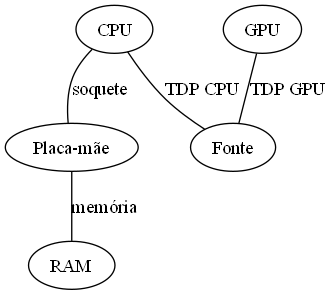
\includegraphics[width=0.5\textwidth]{imagens/grafo-restricoes.png}
  \\\textbf{Fonte:} Elaborada pelo autor
  \label{fig:grafo_restricoes}
\end{figure}
\FloatBarrier

% \FloatBarrier
% \begin{figure}[!htbp]
%   \centering
%   \caption{Grafo de Restrições do Sistema Proposto}
%   %scale redimensiona a figura.
%   %1.5 = 150% do tamanho original
%   %1 = 100% do tamanho original
%   %0.20 = 20% do tamanho original
%   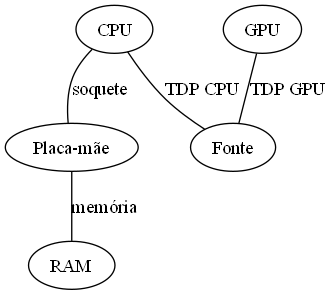
\includegraphics[scale=0.3]{imagens/grafo-restricoes.png}
%   \\\textbf{Fonte:} Elaborada pelo autor
%   \label{fig:exemplo}
% \end{figure}
% \FloatBarrier

Essa estrutura revela que a Fonte é um vértice de alta centralidade no grafo, pois está conectada tanto
à CPU quanto à GPU, de modo que qualquer alteração no domínio de um desses componentes pode propagar
restrições para o domínio da Fonte. A Placa-mãe, por sua vez, é o vértice que medeia a compatibilidade entre CPU e RAM,
funcionando como ponto de articulação da rede de restrições. Esse grafo é o objeto sobre o qual os algoritmos de busca
e propagação operam, cuja complexidade computacional é analisada na seção seguinte.

% ============================================================
\section{Complexidade Computacional}
\label{sec:complexidade}
% ============================================================

A teoria da complexidade computacional ocupa-se da classificação de problemas de decisão segundo
os recursos algorítmicos, principalmente tempo de execução e espaço de memória, exigidos para sua resolução \cite{Cormen2001}.
Dentro desse arcabouço, a classe P reúne os problemas para os quais existem algoritmos determinísticos
de tempo polinomial, considerados eficientes e tratáveis mesmo para entradas de grande escala.
A classe NP, por sua vez, abrange os problemas cuas soluções propostas podem ser verificados em tempo polinomial
por uma máquina determinística, ainda que não se conheça, até o presente, algoritmo eficiente para encontrá-las \cite{Sipser2012}.
A questão sobre a relação entre essas duas classes, se $P = NP$, permanece em aberto e constitui
o problema não resolvido de maior relevância para a ciência da computação teórica, razão pela qual o
\textit{Clay Mathematics Institute} o incluiu entre os sete Problemas do Milênio \cite{Sipser2012}.

O interior da classe NP não é uniforme. A literatura demonstra a existência de subclasses com diferentes
graus de dificuldade, incluindo problemas resolúveis em tempo subexponencial por meio de não-determinismo limitado \cite{Papadimitriou1996}.
O CSP, contudo, não se enquadra nessas classes intermediárias, situando-se no topo da hierarquia como um problema NP-completo \cite{Sipser2012}.
Um problema é classificado como NP-completo quando pertence a NP e todo problema NP se reduz
a ele em tempo polinomial, essa classificação pode ser estabelecida por redução polinomial a partir
do Problema da Satisfabilidade Booleana (SAT), um dos problemas canônicos de NP-completude \cite{Cormen2001,Sipser2012}.
Consequentemente, se qualquer problema NP-completo admitisse solução em tempo polinomial,
toda classe NP colapsaria em P \cite{Sipser2012}.

\subsection{Implicações para o Domínio de Hardware}
Essa natureza NP-completa impõe restrições severas à arquitetura de qualquer sistema de verificação
de compatibilidade de \textit{hardware} fundamentado em CSP. A primeira limitação é de ordem temporal,
a avaliação exaustiva de todas as combinações interdependentes de componentes é inviável na prática em razão
da explosão combinatória intrínseca à classe \cite{Sipser2012,Cormen2001}. Para ilustrar concretamente, considere
que cada categoria de componente possui em média 50 modelos disponíveis no catálogo do sistema. Com cinco
categorias (CPU, Placa-mãe, RAM, GPU e Fonte), a avaliação por força bruta implicaria examinar $50^5 = 312.500.000$ atribuições
candidatas antes de encontrar uma solução válida no pior caso. Esse número cresce exponencialmente à medida
que o catálogo se expande, tornando a abordagem inviável em tempo hábil.

A segunda limitação é de ordem espacial, estratégias alternativas baseadas no mapeamento
estático e exaustivo de regras lógicas condicionais, codificando explicitamente cada restrição de \textit{hardware}
por meio de estruturas if-else ou tabela de decisão, não contornam o problema, pois a representação de funções
lógicas complexas por árvores de decisão pode exiger espaço de tamanho exponencial \cite{Jukna1999}. Diante
dessas limitações, a abordagem padrão para tornar CSPs tratáveis na prática é a busca sistemática
com retrocesso combinada com técnicas de propagação de restrições, que reduzem o espaço efetivo
de busca de forma incremental.

\section{Algoritmos de Busca e Backtracking}
\label{sec:backtracking}

\subsection{Busca em Espaço de Atribuições}
Dado o grafo de restrições e a complexidade NP-completa do CSP, é necessário um algoritmo
de busca sistemática que explore o espaço de atribuições de forma inteligente,
sem enumerar cegamente todas as combinações possíveis. O ponto de partida é o conceito
de atribuição parcial, uma função que associa valores a um subconjunto das variáveis,
podendo ser progressivamente estendida até uma atribuição completa \cite{Russell2010}.
A ideia central dos algoritmos de busca para CSP é construir a atribuição incrementalmente,
verificando consistência a cada passo e abandonando ramos da árvore de busca assim que
uma inconsistência é detectada.

\subsection{Backtracking}
O algoritmo de \textit{backtracking} é o método fundamental de busca para CSPs \cite{Russell2010,Kumar1992}.
Ele percorre recursivamente a árvore de atribuições, em cada nível da recursão, seleciona uma variável
ainda não atribuída, tenta cada valor do seu domínio na ordem disponível, verifica se esse valor é consistente
com as restrições envolvendo as variáveis já atribuídas e recua (\textit{backtrack}) ao encontrar uma inconsistência.
O pseudocódigo do algoritmo é apresentado a seguir:

\begin{algorithm}[hbtp]
  \caption{Algoritmo de Busca por Backtracking para CSP}\label{alg:backtracking}
  \vspace{2mm} % Dá um respiro entre o título e a linha
  \hrule % Desenha a linha superior
  \vspace{2mm} % Dá um respiro entre a linha e o código

  \begin{algorithmic}[1]
    \Function{Backtracking-Search}{$csp$}
    \State \Return \Call{Backtrack}{$\emptyset, csp$}
    \EndFunction
    \Statex
    \Function{Backtrack}{$atribuicao, csp$}
    \If{$atribuicao$ está completa}
    \State \Return $atribuicao$
    \EndIf
    \State $var \gets$ \Call{Selecionar-Variavel-Nao-Atribuída}{$csp$}
    \ForAll{$valor$ em \Call{Ordenar-Valores}{$var, atribuicao, csp$}}
    \If{$valor$ é consistente com $atribuicao$ dado $csp$}
    \State adicionar $\{var = valor\}$ à $atribuicao$
    \State $resultado \gets$ \Call{Backtrack}{$atribuicao, csp$}
    \If{$resultado \neq$ falha}
    \State \Return $resultado$
    \EndIf
    \State remover $\{var = valor\}$ da $atribuicao$
    \EndIf
    \EndFor
    \State \Return falha
    \EndFunction
  \end{algorithmic}

  \vspace{2mm}
  \hrule % Desenha a linha inferior
  \vspace{2mm}
  \fonte{Adaptado de: \textcite{Russell2010}} % Adiciona a fonte padrão ABNT. Se o comando \fonte der erro no seu template, use apenas: Fonte: O autor (2026).
\end{algorithm}


A complexidade de pior caso do \textit{backtracking} puro é $O(d^n)$, na qual $d$ é o tamanho
máximo dos domínios e $n$ é o número de variáveis, reiterando a inviabilidade para instâncias grandes
sem otimizações complementares \cite{Russell2010}.

\subsection{Forward Checking}
Uma primeira melhoria ao backtracking puro é o \textit{forward checking} \cite{Dechter2003}.
Ao atribuir um valor à variável $X_i$, o algoritmo imediatamente examina cada variável $X_j$, ainda
não atribuída que compartilha uma restrição com $X_i$ e remove de $Dom(X_j)$ todos os valores que se tornam
inconsistentes com a atribuição de $X_i$. Se algum domínio $X_j$ se torna vazio, o algoritmo detecta
a falha antecipadamente e recua, sem precisar explorar o ramo até o fim.

Aplicando ao domínio de \textit{hardware}, ao selecionar uma CPU com soquete AM5,
o \textit{forward checking} percorre os vizinhos de CPU no grafo de restrições e remove do domínio
de Placa-mãe todos os modelos com soquete incompatível com AM5, antes mesmo de tentar atribuir um valor
a Placa-mãe. Essa poda antecipada reduz significativamente o número de atribuições exploradas.
Contudo, o \textit{forward checking} verifica apenas os vizinhos diretos da variável recém-atribuída,
sem propagar as consequências dessas remoções para variáveis mais distantes no grafo. A forma mais
completa e eficiente de propagação, que garante consistência global na rede, é o Algoritmo AC-3.

\section{Propagação de Restrições e Algoritmo AC-3}
\label{sec:ac3}
A principal técnica para contornar a explosão combinatória é a propagação de restrições,
realizada por algoritmos de consistência. O mais consolidado na literatura é o AC-3
(\textit{Arc Consistency Algorithm 3}), proposto por \cite{Mackworth1977}, cujo objetivo é garantir
a consistência de arco em redes de restrições binárias \cite{Kumar1992}. Diz-se que um arco
$(X_i, X_j)$ é consistente quando, para todo valor $v \in Dom(X_i)$, existe ao menos um valor
$w \in Dom(X_j)$ tal que a atribuição ${X_i = v, X_j = w}$ satisfaz a restrição entre as duas variáveis.

O algoritmo mantém uma fila de arcos a examinar e, para cada par de variáveis relacionadas,
remove do domínio da variável os valores que não encontram suporte em nenhum valor do domínio da
variável vizinha. Cada remoção dispara a reinserção dos arcos afetados na fila, propagando
a mudança pela rede até o ponto de estabilidade, em que nenhuma redução adicional é possível \cite{Russell2010}.
Assumindo um CSP com $n$ variáveis, domínios de tamanho máximo $d$ e $c$ restrições binárias, a complexidade
de pior caso do AC-3 é $O(cd^3)$ \cite{Russell2010}.

\subsection{Aplicação ao Domínio de Hardware}
Para ilustrar a execução do AC-3 no sistema proposto, considera-se o cenário
em que o usuário seleciona um processador com soquete AM5. A Figura~\ref{fig:ac3_execucao}
apresenta os quatro passos da execução do algoritmo sobre o grafo de restrições
formado pelas variáveis Processador e Placa-mãe.

\FloatBarrier
\begin{figure}[!htbp]
  \centering
  \caption[Execução do AC-3]{Execução passo a passo do AC-3 no grafo de hardware}
  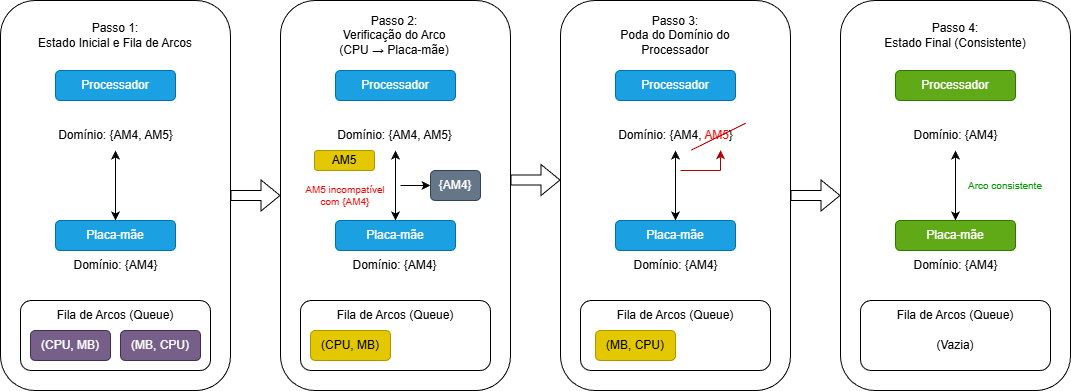
\includegraphics[width=1\textwidth]{imagens/execucao-passo-a-passo-ac-3 (2).png}
  \\\textbf{Fonte:} Elaborada pelo autor
  \label{fig:execucao_ac3}
\end{figure}
\FloatBarrier

No \textbf{Passo 1}, o estado inicial é estabelecido: o domínio do Processador
contém dois valores, AM4 e AM5, e o domínio da Placa-mãe contém apenas AM4.
A fila de arcos é inicializada com os dois arcos direcionados da restrição
bínária: (CPU, MB) e (MB, CPU).

No \textbf{Passo 2}, o arco (CPU, MB) é retirado da fila para verificação.
O algoritmo examina cada valor do domínio do Processador e verifica se existe,
no domínio da Placa-mãe, ao menos um valor que satisfaça a restrição de soquete.
Para o valor AM4, existe suporte no domínio da Placa-mãe. Para o valor AM5,
não existe suporte, pois a placa disponível suporta apenas AM4 --- a incompatibilidade
é identificada.

No \textbf{Passo 3}, o valor AM5 é removido do domínio do Processador por não
possuir suporte na variável vizinha. O arco (MB, CPU) é reinserido na fila para
que o algoritmo verifique se as remoções realizadas tornaram algum valor da
Placa-mãe inconsistente.

No \textbf{Passo 4}, o arco (MB, CPU) é processado. O valor AM4 da Placa-mãe
encontra suporte no valor AM4 do Processador, portanto nenhuma remoção adicional
é necessária. A fila esvazia e o algoritmo encerra no ponto de estabilidade:
ambas as variáveis possuem domínios consistentes com a restrição, sem necessidade
de explorar nenhuma atribuição completa por força bruta.

O resultado ilustra o mecanismo central do motor de inferência: uma única seleção
do usuário dispara a propagação de restrições por toda a rede, reduzindo os
domínios disponíveis de forma incremental e em tempo real \cite{Mackworth1977,Russell2010}.

\section{Sistema Especialista}
\label{sec:sistema-especialista}
Um Sistema Especialista (SE) é um programa de computador projetado para simular o raciocínio de um
especialista humano em um domínio restrito e bem definido \cite{Russell2010}. Diferentemente de sistema
de propósito geral, um SE concentra seu conhecimento em um domínio específico e é capaz de resolver
problemas nesse domínio com nível de competência comparável ao de um especialista humano \cite{Jackson1998}.
Sua arquitetura é composta por três elementos centrais: a base de conhecimento, que armazena fatos
e regras sobre o domínio, o motor de inferência, que aplica essas regras aos fatos disponíveis
para derivar conclusões e a interface de explicação, que permite ao sistema justificar
suas respostas ao usuário \cite{Russell2010}.

O motor de inferência pode operar segundo encadeamento progressivo (\textit{forward chaining}),
partindo dos fatos conhecidos em direção a conclusões, ou encadeamento regressivo (\textit{backward chaining}),
partindo de uma hipótese e verificando se os fatos disponíveis a sustentam \cite{Russell2010}.
No sistema proposto, o motor opera predominantemente em modo progressivo: a cada seleção de componente
pelo usuário, o sistema propaga as restrições a partir desse novo fato para derivar quais opções
permanecem válidas.

\subsection{Explanation Facilities}
A capacidade de justificar o próprio raciocínio, denominada na literatura como
\textit{explanation facility}, é o que distingui fundamentalmente um SE de um mecanismo
de filtragem comum \cite{Clancey1983}. Segundo \cite{Clancey1983}, essa capacidade exige que o sistema
mantenha não apenas as conclusões derivadas, mas também a cadeia de regras e restrições que
levou a cada conclusão, de modo que possa reconstruir e comunicar o raciocínio em linguagem
acessível ao usuário. Um mecanismo de filtragem simples responde apenas à pergunta "quais opções são válidas?",
apresentado resultados sem elaboração. Um SE com \textit{explanation facility} responde também à pergunta
"por que as demais opçõs são inválidas?", articulando a regra específica que foi violada.

No contexto do sistema proposta, essa capacidade se manifesta da seguinte forma, ao bloquear a seleção de um módulo DDR4 após
a escolha de uma CPU AM5, o sistema não se limita a remover o componente da lista de opções,
ele apresenta ao usuário uma justificativa explícita como "Este módulo de memória é incompatível: a placa-mãe
compatível com o processador selecionada suporta exclusivamente DDR5 e este módulo é DDR4". Essa explicação
transforma cada bloqueio em uma oportunidade de aprendizado sobre as restrições físicas do \textit{hardware}.

\subsection{Inteligência Artificial Explicável (XAI)}
O problema identificado por \textcite{Clancey1983}, a necessidade de sistemas inteligentes justificarem seu
raciocónio ao usuário, permaneceu latente por décadas e ressurgiu com força renovada no contexto da Inteligência Artificial (IA)
moderna sob o nome de XAI (\textit{eXplainable Artificial Intelligence}), ou Inteligência Artificial Explicável. \textcite{Arrieta2020}
definem XAI como o conjunto de processos e técnicas que permitem que modelos de inteligência artificial produzam
resultados compreensíveis por seres humanos, especialmente por usuários finais sem formação técnica em IA.
Os autores identificam a explicabilidade como uma necessidade crítica para a adoção prática de sistemas de IA em domínios
sensíveis, argumentando que um sistema que apenas produz resultados sem justificá-los não gera confiança suficiente para
ser adotado em decisões reais.

A distinção central que o campo de XAI estabelece é entre sistemas caixa-preta (\textit{black-box}), cujo processo
de decisão interno é opaco ao usuário, e sistemas transparentes, cujo raciocínio pode ser inspecionado e compreendido \cite{Arrieta2020}.
Sistemas especialistas baseados em CSP pertencem naturalmente à segunda categoria, as variáveis, os domínios e as restrições
são explícitos e auditáveis e cada decisão de bloqueio pode ser rastreada até a restrição específica que a originou.
Nesse sentido, o motor de inferência CSP/AC-3 proposto neste trabalho é intrinsecamente explicável por \textit{design}, não por
técnica de pós-processamento, mas pela própria natureza simbólica do modelo. Isso posiciona o sistema proposto em alinhamento com
os princípios contemporâneos de XAI, cada resultado produzido pelo motor de inferência é acompanhado da justificativa técnica
que o fundamenta, tornando o processo de validação de \textit{hardware} transparente e auditável pelo usuário.

\subsection{Mapeamento ao Sistema Proposto}
O sistema proposto neste trabalho se enquadra na categoria de sistemas especialistas baseados em restrições.
Os três componentes arquiteturais do SE mapeiam diretamente à implementação: a base de conhecimento corresponde
à camada de dados que armazena as especificações técnicas dos componentes e as regras de compatibilidade modeladas
como restrições do CSP; o motor de inferência corresponde ao algoritmo AC-3 implementado na camada de lógica da aplicação,
responsável por propagar restrições e podar domínios a cada interação do usuário; e a interface de explicação corresponde
aos alertas técnicos e educativos exibidos na camada de apresentação, que comunicam ao usuário não apenas quais componentes
são bloqueados, mas as razões físicas e técnicas subjacentes a cada bloqueio \cite{Jackson1998}.

\section{Dimensão Educativa em Sistemas Especialistas}
\label{sec:dimensao-educativa}
O caráter educativo do sistema proposto não decorre da adoção de uma arquitetura de aprendizagem  adaptativa,
mas da forma como o motor de inferência comunica suas conclusões ao usuário. Para delimitar com precisão
essa dimensão, é necessário distinguir três categorias de sistemas que operam sobre domínios de conhecimento restrito:
os mecanismos de filtragem, os Sistemas Tutores Inteligentes (STI) e os Sistemas Especialistas com interface educativa.


\subsection{Mecanismo de Filtragem versus Sistema com Explicação}
Um mecanismo de filtragem tradicional opera sobre um conjunto de dados e retorna os elementos que
satisfazem determinados critérios, sem qualquer elaboração sobre o processo de decisão. No contexto de compatibilidade de
\textit{hardware}, um filtro responde à pergunta "quais componentes são compatíveis com minha seleção atual?", apresentando
uma lista de resultados válidos e ocultando ou desabilitando os inválidos, sem indicar o motivo da exclusão. Plataformas comerciais
como o \textit{PC Part Picker} operam predominantemente nesse paradigma: informam a incompatibilidade, mas raramente
explicam a regra física que a origina.

A limitação pedagógica desse modelo é nítida: o usuário aprende o que não pode fazer, mas não aprende o motivo.
Cada bloqueio silencioso é uma oportunidade de aprendizagem perdida \cite{Clancey1983}. Um sistema que apenas
filtra não transfere conhecimento, apenas restringe escolhas.

\subsection{Sistemas Tutores Inteligentes}
Sistemas Tutores Inteligentes (STI) representam o paradigma mais sofisticado de instrução mediada por computador.
Sua arquitetura formal é composta por quatro modelos interdependentes: o modelo de domínio, que representa o
conhecimento a ser ensinado; o modelo de estudante, que representa o estado de conhecimento individual do aprendiz e é
atualizado continuamente com base em seus erros e acertos; o modelo pedagógico, que define as estratégias de instrução e adaptação;
e o modelo da interface, que define como o conteúdo é apresentado \cite{Woolf2008}. O elemento central que distingue
um STI de outros sistemas é o modelo de estudante, ele exige que o sistema mantenha um perfil persistente por usuário, rastreando o histórico
de interações ao longo de múltiplas sessões para personalizar a instrução \cite{Anderson1995}.

O sistema proposto neste trabalho não implementa a arquitetura de um STI. Não há rastreamento de sessões individuais,
não há perfil persistente de usuário e não há adaptação sequencial de conteúdo baseado em histórico. Essa delimitação
é intencional, pois o objetivo é criar um sistema especialista com interface educativa, que se concentra na explicação
de cada bloqueio como uma oportunidade de aprendizagem, sem a complexidade adicional de um modelo de estudante adaptativo.

\subsection{Sistema Especialista Educacional}
O sistema proposto se enquadra na categoria de Sistema Especialista Educacional, um SE dotado de \textit{explanation facility}
cuja interface é projetado com objetivo pedagógico explícito. A distinção em relação a um SE convencional reside na forma como
as conclusões são comunicadas. Enquanto um SE padrão pode simplesmente retornar um resultado binário (compatível ou incompatível),
um SE educacional articula a cadeia de raciocínio que levou aquela conclusão em linguagem acessível ao usuário \cite{Clancey1983,Jackson1998}.

No sistema proposto, essa dimensão educativa se manifesta de forma precisa e delimitada: ao detectar uma violação de restrição
via propagação AC-3, o sistema não limita a bloquear o componente incompatível, ele apresenta ao usuário uma justificativa explícita
que identifica qual restrição foi violada e por qual razão técnica. Por exemplo, ao tentar selecionar um módulo DDR4 após escolher
umas CPU com plataforma AM5, o sistema exibe: "Este módulo de memória é incompatível: a placa-mãe compatível com o processador selecionado
suporta exclusivamente DDR5, e este módulo utiliza o padrão DDR4". Essa explicação transforma cada bloqueio em uma oportunidade de
aprendizagem sobre os princípios físicos que regem a montagem de computadores, sem requerer qualquer cadastro, histórico ou personalização
por parte do usuário.

Essa abordagem é pedagogicamente coerente com público-alvo do sistema, o usuário leigo que realiza uma única sessão de configuração,
para quem a explicação contextualizada e imediata é mais eficaz do que qualquer mecanismo de adaptação baseado em histórico. O adjetivo
"Educacional" no título do trabalho refere-se precisamente a essa capacidade de instruir o usuário sobre as restrições do domínio no exato
momento em que elas se tornam relevantes para sua decisão.

\section{Arquitetura de Software Orientada a Serviços}
\label{sec:arquitetura-software}

\subsection{Arquitetura em Camadas}
A arquitetura de \textit{software} compreende o conjunto de decisões estruturais fundamentais que definem a organização
de um sistema, as responsabilidades de seus componentes e as interfaces através das quais eles se comunicam \cite{Fowler2002}.
Um dos padrões arquiteturais mais consolidados na engenharia de \textit{software} é a arquitetura em camadas, que organiza
o sistema em níveis hierárquicos de abstração, cada um com responsabilidades bem delimitadas e comunicando-se apenas com
a camada imediatamente adjacente \cite{Fowler2002}.

As três camadas clássicas são: a camada de apresentação, responsável pela interação com o usuário e pela exibição de informações,
a camada de lógica de negócio, responsável pelo processamento, pelas regras do domínio e pelas decisões da aplicação e a camada de dados,
responsável pelo armazenamento, recuperação e persistência de informações \cite{Fowler2002}. Essa separação aumenta a manutenibilidade
do sistema, alterações em uma camada não propagam mudanças para as demais, e facilita a testabilidade, permitindo que cada camada seja
verificada de forma independente.

\subsection{REST como Estilo Arquitetural}
A comunicação entre camadas distribuídas em sistemas \textit{web} segue estilos arquiteturais que impõem restrições sobre
como os componentes interagem. O estilo mais amplamente adotado é o REST (\textit{Representational State Transfer}), definido por
\cite{Fielding2000} em sua tese de doutorado como um conjunto de seis princípios arquiteturais para sistemas distribuídos baseados
em rede.

Os princípios mais relevantes para o sistema proposto são:

O princípio de cliente-servidor, que estabelece a separação entre a interface do usuário e o armazenamento e processamento de dados,
permitindo que cada lado evolua de forma independente. No sistema proposto, o cliente e o servidor evoluem independentemente, a interface
pode ser redesenhada sem alterar o motor CSP, e o motor CSP pode ser otimizado sem alterar a inteface.

O princípio \textit{stateless} (sem estado), que estabelece que cada requisição enviado pelo cliente ao servidor deve conter
todas as informações necessárias para ser compreendida e processada, sem depender de contexto ou sessão armazenada no servidor
entre requisições \cite{Fielding2000}. No contexto do sistema proposto, isso significa que cada chamada à \textit{API} carrega o
estado atual completo das seleções do usuário, quais componentes foram escolhidos e quais permanecem em aberto e o motor CSP
executa a propagação de restrições a partir desse estado, sem manter sessão persistente no servidor. Essa característica garante
escalabilidade e simplicidade operacional.

O princípio da interface uniforme, que estabelece que a comunicação entre o cliente e servidor deve seguir um contrato padronizado,
baseado em recursos identificados por URIs e operações semânticas bem definidas \cite{Richardson2007}. No sistema proposto,
cada categoria de componente e cada conjunto de restrições é exposto como um recurso REST, acessível por operações HTTP padronizadas.

\subsection{Mapeamento ao Sistema Proposto}
A arquitetura do sistema proposto realiza concretamente os princípios da
arquitetura em camadas e do estilo REST, conforme ilustrado na
Figura~\ref{fig:arquitetura_rest}.

\FloatBarrier
\begin{figure}[!htbp]
  \centering
  \caption[Diagrama da arquitetura em três camadas do sistema]{Diagrama da arquitetura em três camadas do sistema}
  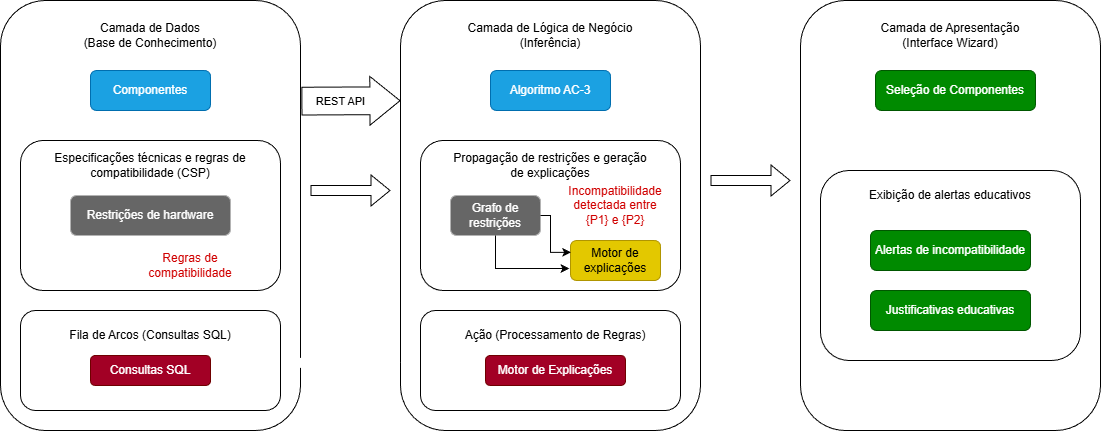
\includegraphics[width=1\textwidth]{imagens/DIAGRAMA REST.png}
  \\\textbf{Fonte:} Elaborada pelo autor
  \label{fig:diagrama_arquitetura}
\end{figure}
\FloatBarrier

A \textbf{camada de dados}, representada no painel esquerdo da figura, armazena
a base de conhecimento do sistema especialista: os modelos de componentes de
\textit{hardware}, as especificações técnicas que constituem as variáveis do CSP,
as restrições de compatibilidade que compõem o conjunto $C$, e as regras de
compatibilidade que fundamentam as decisões do motor de inferência. O acesso
a essa camada é realizado por meio de consultas SQL disparadas pela camada
de lógica de negócio.

A \textbf{camada de lógica de negócio}, representada no painel central, é o
núcleo inteligente do sistema. Após receber uma requisição via \textit{REST API}
contendo o estado atual das seleções do usuário, essa camada executa o
Algoritmo AC-3 sobre o grafo de restrições: identifica os arcos inconsistentes,
poda os domínios das variáveis afetadas e, ao detectar uma incompatibilidade
entre dois componentes $P_1$ e $P_2$, aciona o motor de explicações, que
formula a justificativa técnica a ser apresentada ao usuário. O resultado
do processamento é retornado à camada de apresentação como resposta à
requisição REST.

A \textbf{camada de apresentação}, representada no painel direito, é a interface
\textit{wizard} com a qual o usuário interage diretamente. Ela é responsável
por exibir o catálogo de componentes disponíveis para seleção, apresentar os
alertas de incompatibilidade gerados pelo motor de inferência e comunicar as
justificativas educativas que fundamentam cada bloqueio, transformando o
resultado da validação CSP em uma oportunidade de aprendizagem sobre os
princípios físicos que regem a montagem de computadores.

A separação entre as três camadas garante que o motor de inferência possa ser
mantido e expandido de forma independente da interface de apresentação,
preservando a modularidade arquitetural ao longo do ciclo de desenvolvimento
do sistema \cite{Fowler2002,Fielding2000}.

\section{Trabalhos Relacionados}
Esta seção mapeia o estado da arte em duas frentes: as plataformas comerciais de verificação de compatibilidade
de \textit{hardware} atualmente disponíveis e os trabalhos acadêmicos sobre sistemas especialistas e CSP aplicados
a domínios similares. O objetivo é evidenciar as lacunas existentes nas soluções atuais e posicionar a contribuição do
presente trabalho em relação a elas.

\subsection{Plataformas Comerciais de Compatibilidade de Hardware}
O PC Part Picker é a plataforma de referência global para montagem de computadores. Permite ao usuário
selecionar componentes de um catálogo extenso e verifica automaticamente incompatibilidades entre as pelas
escolhidas \cite{PCPARTPICKER2024}. Quando uma incompatibilidade é detectada, a plataforma exibe um alerta
genérico indicando que os componentes são incompatíveis, mas sem detalhar a regra técnica violada, por exemplo, ao selecionar uma
CPU AM5 com um módulo DDR4, o sistema indica o conflito sem explicar a diferença entre os padrões de memória
ou a razão física da incompatibilidade. Do ponto de vista da teoria de sistemas especialistas, o PC Part Picker
implementa um mecanismo de filtragem sem \textit{explanation facility}, o usuário recebe o resultado da
validação, mas não o raciocínio que o produziu \cite{Clancey1983}.

O Meupc.net é a alternativa nacional mais utilizada no contexto brasileiro, operando de forma similar
ao PC Part Picker com catálogo voltado ao mercado local \cite{MEUPC2024}. Apresenta as mesmas limitações
em termos de explicação, as incompatibilidades são sinalizadas visualmente, mas sem justificativa técnica que
permita ao usuário compreender o princípio de \textit{hardware} subjacente à restrição.

A limitação comum a ambas as plataformas é estrutural, por operaram como mecanismos de filtragem e não
como sistemas especialistas com capacidade explicativa, não transferem conhecimento ao usuário, apenas
restringem escolhas. Um usuário que utiliza PC Part Picker repetidamente aprende quais componentes são
compatíveis entre si, mas não aprende por que são compatíveis, o que o impede de generalizar
o conhecimento adquirido para novas situações de compra.

\subsection{Trabalhos Acadêmicos Relacionados}
Na literatura acadêmica, a aplicação de CSPs a problemas de configuração de produtos é um tema consolidado.
\textcite{Sabin1998} apresentam uma \textit{survey} abrangente sobre sistemas de configuração baseados em CSP,
identificando a modelagem de dependências entre componentes como variáveis e restrições é a abordagem mais
expressiva para domínios com regras de compatibilidade complexas. Os autores demonstram que sistemas de configuração
baseada em CSP superam abordagem baseadas em regras estáticas tanto em expressividade quanto em eficiência de
manutenção de base de conhecimento, resultado diretamente aplicável ao domínio de \textit{hardware} proposto neste trabalho.

\textcite{Mittal1989} introduzem o conceito de \textit{dynamic CSP}, no qual o conjunto de variáveis e restrições
pode ser alterado durante a busca, uma extensão relevante para sistemas de configuração interativos onde o
usuário faz escolhas incrementais, como é o caso do sistema proposto. Essa abordagem sustenta a decisão arquitetural
de propagar restrições a cada interação do usuário, em vez de processar o CSP completo apenas ao final da configuração.

No campo de sistemas especialistas educacionais, \textcite{Nwana1990} discute os requisitos para que um sistema
especialista seja considerado efetivamente educativo, identificando a capacidade de explicação como condição necessária,
mas não suficiente, para a transferência de conhecimento. O autor distingue sistemas que explicam o que de sistemas
\textit{o que} explicam \textit{por que}, argumentando que apenas os últimos têm impacto pedagógico real. Esse
referencial sustenta diretamente a decisão de projeto de exibir não apenas o resultado da validação, mas a regra de
compatibilidade violada em linguagem acessível ao usuário.

Mais recentemente, \textcite{Wang2018} desenvolveram um sistema especialista educacional para apoio ao aprendizado
de classificação botânica em ambiente móvel, demonstrando que sistemas especialistas com \textit{feedback} explicativo
produzem ganhos mensuráveis de aprendizagem em comparação com sistemas que apenas apresentam informação estática.
O estudo é relevante para o presente trabalho por demonstrar empiricamente que a capacidade de explicação, e não
apenas a apresentação de conteúdo, é o fator determinante para o impacto pedagógico de um sistema especialista,
validando a abordagem adotada no sistema de compatibilidade de \textit{hardware} proposto.

\subsection{Posicionamento do Trabalho Proposto}
A análise das plataformas comerciais e dos trabalhos acadêmicos permite identificar com precisão a contribuição do presente
trabalho. Em relação as plataformas comerciais, o diferencial está na \textit{explanation facility}. enquanto PC Part Picker
e Meupc.net sinalizam incompatibilidades sem explicá-las, o sistema proposto articula a regra técnica violada em cada bloqueio,
transformando a interação em uma oportunidade de aprendizagem. Em relação aos trabalhos acadêmicos, a contribuição está na combinação
de três elementos que, individualmente, já são estudados na literatura, CSP como motor de inferência \cite{Sabin1998}, sistema
especialista com capacidade explicativa alinhada a princípios de XAI \cite{Clancey1983,Arrieta2020} e interface educativa
com impacto pedagógico demonstrável \cite{Wang2018}, em um sistema \textit{web} completo validado sobre um domínio concreto
e de relevância prática imediata para o usuário.

% Texto da revisão da literatura, dividido em seções e subseções.


% Este é um exemplo de como usar figuras. Referência cruzada: Figura~\ref{fig:exemplo}

% \FloatBarrier
% \begin{figure}[!htbp]
%   \centering
%   \caption{Exemplo de figura}
%   %scale redimensiona a figura.
%   %1.5 = 150% do tamanho original
%   %1 = 100% do tamanho original
%   %0.20 = 20% do tamanho original
%   
\includegraphics[scale=0.3]{imagens/LogoIF_BRI10}
%   \\\textbf{Fonte:} Elaborada pelo autor
%   \label{fig:exemplo}
% \end{figure}
% \FloatBarrier


% Este é um exemplo de como usar tabelas. Referência cruzada: Tabela~\ref{tab:exemplo}

% \FloatBarrier
% \begin{table}[!htbp]
%   \centering
%   \caption{Exemplo de tabela de 2 colunas}
%   \begin{tabular}{ c | c }
%     \hline
%     \textbf{Coluna 1} & \textbf{Coluna 2} \\ \hline
%     Dado 1a           & Dado 2a           \\ \hline
%     Dado 1b           & Dado 2b           \\ \hline
%     Dado 1c           & Dado 2c           \\ \hline
%     Dado 1d           & Dado 2d           \\ \hline
%   \end{tabular}
%   \\ \vspace{0.2cm}
%   \textbf{Fonte:} Elaborada pelo autor
%   \label{tab:exemplo}
% \end{table}
% \FloatBarrier


% Este é um exemplo de como usar quadros. Referência cruzada: Quadro~\ref{qua:exemplo}

% \FloatBarrier
% \begin{quadro}[!htbp]
%   \centering
%   \caption{Exemplo de quadro}
%   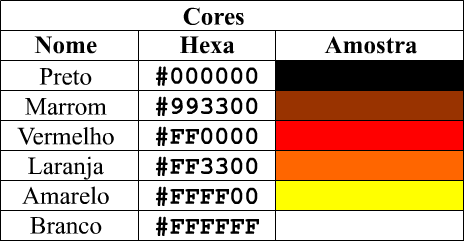
\includegraphics[scale=.7]{imagens/exemploQuadro}
%   \\\textbf{Fonte:} Elaborada pelo autor
%   \label{qua:exemplo}
% \end{quadro}
% \FloatBarrier


% Este é um exemplo de como usar equações. Referência cruzada: Equação~\ref{eq:exemplo}

% \begin{equation}
%   \sum_{i=1}^{n} i = \frac{n(n+1)}{2}
%   \label{eq:exemplo}
% \end{equation}


% Exemplo de inserção de lista de código fonte (\textbf{\textcolor{red}{não use acentos no código!}}):

% \lstinputlisting[language=Java]{fontes/ClasseExemplo.java}



% Este é um exemplo de como inserir texto sem formatação (ambiente verbatim):

% \begin{verbatim}
% 	Texto sem formatação, como espaçamento igual.
% \end{verbatim}


% Exemplo de lista de itens:

% \begin{itemize}
%   \item \textbf{Item 1:} texto...;
%   \item \textbf{Item 2:} texto...;
%         \begin{itemize}
%           \item \textbf{Subitem:} texto...;
%           \item \textbf{Subitem:} texto...;
%           \item \textbf{Subitem:} texto...;
%         \end{itemize}
%   \item \textbf{Item 3:} texto...;
%   \item \textbf{Item n:} texto....
% \end{itemize}


% Exemplo de lista numerada:

% \begin{enumerate}
%   \item \textbf{Item:} texto...;
%   \item \textbf{Item:} texto...;
%         \begin{enumerate}
%           \item \textbf{Subitem:} texto...;
%           \item \textbf{Subitem:} texto...;
%           \item \textbf{Subitem:} texto...;
%         \end{enumerate}
%   \item \textbf{Item:} texto...;
%   \item \textbf{Item:} texto....
% \end{enumerate}


% Exemplos de comandos para texto e referências:

% \begin{itemize}
%   \item Para iniciar um novo parágrafo, basta deixar uma linha em branco no código fonte;
%   \item Não force o compilador a pular mais de uma linha, pois terá influência negativa na composição do documento;
%   \item Sempre deixe o \LaTeX\ realizar a formatação de parágrafos e posicionamento de elementos;
%   \item Utilização de aspas simples (abertura \verb|`|, fechamento \verb|'|): `Texto entre aspas simples';
%   \item Utilização de aspas duplas (abertura \verb|``|, fechamento \verb|''|): ``Texto entre aspas duplas'';
%   \item Negrito (comando \verb|\textbf|): \textbf{texto em negrito};
%   \item Itálico (comando \verb|\textit|): \textit{texto em itálico};
%   \item Sublinhado (comando \verb|\underline|): \underline{texto sublinhado};
%   \item Negrito e itálico (usar comandos juntos): \textbf{\textit{texto em negrito e itálico}};
%   \item Alterar cor do texto (comando \verb|\textcolor{cor}{texto}|):
%         \begin{itemize}
%           \item Exemplo \verb|\textcolor{red}{texto}|: \textcolor{red}{texto vermelho};
%           \item Exemplo \verb|\textcolor[RGB]{255, 102, 0}|: \textcolor[RGB]{255, 102, 0}{texto laranja};
%           \item Exemplo \verb|\textcolor[HTML]{006AD7}|: \textcolor[HTML]{006AD7}{texto azul};
%         \end{itemize}
%   \item Ambiente matemático inline (comando \verb|$ expressão $|): $s = x^2-2x +1$;
%   \item Referência normal (comando \verb|\cite|):
%         \begin{itemize}
%           \item \cite{Agaisse1995};
%           \item \cite{Abedi2014};
%           \item \cite{BtNomenclature2016};
%         \end{itemize}
%   \item Referência normal com mais de uma obra (comando \verb|\cite|):
%         \begin{itemize}
%           \item \cite{Abedi2014, Agaisse1995};
%           \item \cite{AgapitoTenfen2014, BtNomenclature2016, Nelson2014};
%         \end{itemize}
%   \item Referência nome e ano (comando \verb|\citeauthorandyear|):
%         \begin{itemize}
%           \item \textcite{Agaisse1995};
%           \item \textcite{Abedi2014};
%           \item \textcite{BtNomenclature2016};
%         \end{itemize}
% \end{itemize}


% Exemplo 1 de citação direta:

% \begin{citacao}
%   Os 20 aminoácidos usualmente encontrados como resíduos em proteínas contém um grupo $\alpha$-carboxil, um grupo $\alpha$-amino e um grupo R distinto substituído no átomo de carbono $\alpha$. O átomo de carbono $\alpha$ de todos os aminoácidos, com exceção da glicina, é assimétrico e, portanto, os aminoácidos podem existir em pelo menos duas formas estereoisoméricas. Somente os estereoisômeros L, com uma configuração relacionada à configuração absoluta da molécula de referência L-gliceraldeído, são encontrados em proteínas \cite[p. 81]{Nelson2014}.
% \end{citacao}

% Exemplo 2 de citação direta:

% \begin{citacao}
%   \textit{These various insecticidal proteins are synthesized during the stationary phase and accumulate in the mother cell as a crystal inclusion which can account for up to 25\% of the dry weight of the sporulated cells. The amount of crystal protein produced by a B. thuringiensis culture in laboratory conditions (about 0.5 mg of protein per ml) and the size of the crystals (24) indicate that each cell has to synthesize $10^6$ to $2 \times 10^6$ $\delta$-endotoxin molecules during the stationary phase to form a crystal} \cite[p. 1]{Agaisse1995}.
% \end{citacao}

% Exemplo de nota de rodapé\footnote{Essa é uma nota de rodapé!}.
\chapter{Materiais e métodos}
\label{cap:03}
De acordo com a natureza e os objetivos do presente trabalho, foram adotadas as seguintes metodologias de pesquisa para
embasar o desenvolvimento do sistema especialista educacional proposto.

\section{Natureza da Pesquisa}
\label{sec:natureza-pesquisa}

\subsection{Bibliográfica}
Durante o desenvolvimento deste trabalho, aplica-se a metodologia bibliográfica, por meio da qual foi realizada
a análise de materiais já publicados. Para isso, fez-se necessária a avaliação e fundamentação sobre os conteúdos
consultados podendo eles ser "de livros, periódicos, documentos, textos,
mapas, fotos, manuscritos e, até mesmo, de material
disponibilizado na internet etc" \cite{fontelles2009}.

Em primeira instância, a pesquisa foi conduzida com a definição dos temas e objetivos necessários, com o intuito de identificar
os assuntos que sustentam a narrativa do trabalho, esclarecendo quais pontos são úteis e relevantes para a pesquisa. Os temas
centrais investigados foram: Problemas de Satisfação de Restrições (CSP), algoritmos de propagação de restrições,
sistemas especialistas, inteligência artificial explicável (XAI), sistemas tutores inteligentes e arquitetura de software
orientada a serviços. Além disso, foi necessário delimitar um período para a seleção das fontes, priorizando materiais mais
recentes, sem desconsiderar obras clássicas e fundamentais para o domínio, como os trabalhos de \textcite{Clancey1983},
\textcite{Mackworth1977} e \textcite{Russell2010}, dada a relevância teórica permanente de tais referências.

Após essa etapa inicial, foram selecionadas como principais bases de busca o Google Scholar e o Portal de Periódicos da CAPES,
acessado por meio do sistema CAFe (Comunidade Acadêmica Federada), em razão de sua vasta cobertura de artigos científicos,
livros, teses, dissertações e demais produções acadêmicas indexadas. Foram também realizadas buscas direcionadas em portais de
conferências e periódicos especializados em inteligência artificial, engenharia de \textit{software} e sistemas de informação.

Dado o volume de resultados retornados, realizou-se uma triagem dos materiais recuperados por meio da leitura de resumos.
Os materiais considerados relevantes foram incluídos, nos casos de dúvidas quando à permanência, procedeu-se a uma leitura
mais minuciosa. Após a seleção, foi realizada uma análise detalhada dos materiais e a síntese das informações coletadas.

Por fim, todas as pesquisas e extrações de informações foram revisadas, de modo a evitar erros e má interpretação. A revisão foi
conduzida em duas etapas, com releitura do material, da síntese e da extração de informação, resultando em ajustes quando
necessário e garantindo a qualidade e a precisão das informações utilizadas ao longo do trabalho.

\subsection{Aplicada}
A pesquisa aplicada orienta o desenvolvimento prático de compatibilidade, cujo produto é um sistema especialista educacional
para validação de compatibilidade de \textit{hardware}. Segundo \textcite{gerhardt2009}, a pesquisa aplicada tem como objetivo
gerar conhecimento para aplicação prática e dirigidos à solução de problemas específicos. Neste contexto, os fundamentos
teóricos levantados pela pesquisa bibliográfica, notadamente o formalismo de CSP, o algoritmo AC-3 e os princípios de
sistemas especialistas com \textit{explanation facility}, foram diretamente empregados na concepção e implementação do
sistema proposto.

Essa abordagem permitiu que as decisões arquiteturais e de projeto fossem fundamentadas em evidências da literatura, como a
adoção da arquitetura em três camadas \cite{Fowler2002}, o estilo REST para comunicação entre camadas \cite{Fielding2000}
e o algoritmo AC-3 como motor de inferência \cite{Mackworth1977}, garantindo o alinhamento entre os resultados práticos
obtidos e o referencial teórico consolidado.

\section{Materiais}
\label{sec:materiais}

\subsection{Equipamentos}
Para a realização do desenvolvimento, codificação e testes do sistema, foi utilizado um computador com processador Ryzen 7 5700X, 32GB de
memória RAM, placa de vídeo AMD Radeon RX 7600 e sistema operacional Windows 11. Esses recursos foram suficientes para executar o ambiente de
desenvolvimento, o servidor de aplicação, o sistema de gerenciador de banco de dados e os navegadores necessários para a validação da
interface.

\subsection{Softwares}
Para o desenvolvimento do sistema foram utilizadas ferramentas de \textit{software} selecionadas com base em sua adequação técnica ao
projeto, disponibilidade gratuita ou de código aberto e familiaridade prévia do desenvolvedor.

\section{Ferramentas Utilizadas}

\subsection{Visual Studio Code}
O Visual Studio Code (VS Code) é um editor de código-fonte desenvolvido pela Microsoft, disponível gratuitamente para sistemas
operacionais Windows, Linux e MacOS. Por meio de extensões, a ferramenta agrega funcionalidades como depuração, controle de versão,
terminal integrado e suporte a diversas linguagens de programação, aproximando-se de um ambiente de desenvolvimento integrado (IDE).

No presente trabalho, o VS Code foi utilizado como ambiente principal de desenvolvimento, tanto para codificação do \textit{backend}
e do \textit{frontend} quanto para a edição e compilação do documento LaTeX deste trabalho, por meio da extensão LaTeX Workshop.
A escolha pela ferramenta deve-se à sua leveza, à vasta disponibilidade de extensões relevantes para o ecossistema adotado
e ao conhecimento prévio do desenvolvedor.

\subsection{Node.js e NestJS}
O Node.js é um ambiente de execução JavaScript de código aberto e multiplataforma, construído sobre o motor V8 do Google Chrome,
que permite a execução de código JavaScript no lado do servidor, sendo amplamente empregado no desenvolvimento de aplicações \textit{web}
escaláveis e de alta performance. O NestJS é um \textit{framework} para desenvolvimento de aplicações server-side organizado em módulos, \textit{controllers}
e \textit{services}. Essa estrutura favorece a separação de responsabilidades e a manutenibilidade do código, alinhando-se diretamente
aos princípios da arquitetura em camadas descrito por \textcite{Fowler2002}.

No contexto do sistema proposto, o Node.js com NestJS compõe a camada de lógica de negócio, sendo o responsável por receber as requisições
da interface, executar o algoritmo AC-3 sobre o grafo de restrições de \textit{hardware} e retornar ao cliente os resultados da validação
acompanhados das justificativas educativas correspondentes.

\subsection{PostgreSQL e Docker}
O PostgreSQL é um banco de dados relacional de código aberto, com suporte a transações, multiplataforma e amplamente utilizado em aplicações
\textit{web} de diferentes escalas. A escolha por esse sistema deve-se à sua robustez, à sua conformidade com o padrão SQL e à facilidade
de integração com ecossistemas Node.js.

No sistema proposto, o PostgreSQL é utilizado para armazenar a base de conhecimento do sistema especialista: os modelos de componentes de
\textit{hardware}, suas especificações técnicas e as regras de compatibilidade que compõem o conjunto de restrições do CSP. Essas informações
são consultadas pela camada de lógica de negócio a cada execução do algoritmo AC-3.

O provisionamento do banco de dados foi realizado por meio do Docker, uma plataforma de código aberto para criação e execução de contêineres
de \textit{software}. A utilização do Docker permite que o ambiente do banco de dados seja definido de forma declarativa e reproduzível,
garantindo consistência entre os ambientes de desenvolvimento e produção sem a necessidade de instalação direta do PostgreSQL no sistema operacional.

\subsection{DBeaver}
O DBeaver é uma ferramenta de administração de banco de dados de código aberto e multiplataforma, compatível com diversos sistemas gerenciadores,
incluindo o PostgreSQL. A ferramenta oferece uma interface visual para a execução de consultas SQL, navegação entre tabelas, modelagem de dados e
exportação de resultados.

No presente trabalho, o DBeaver foi utilizado para o auxílio na administração e manipulação do banco de dados durante
o desenvolvimento, permitindo a inspeção e validação dos dados cadastrados na base de conhecimento do sistema especialista.

\subsection{Next.js}
O Next.js é um \textit{framework} de código aberto para o desenvolvimento de aplicações \textit{web} construído sobre o React, desenvolvido
e mantido pela Vercel. O \textit{framework} oferece recursos como renderização híbrida, roteamento baseado em sistemas de arquivos e
suporte nativo a APIs, facilitando o desenvolvimento de aplicações \textit{web} com uma única base de código.

No presente trabalho, o Next.js foi utilizado para o desenvolvimento da camada de apresentação do sistema, implementada como uma interface
no formato \textit{wizard} que guia o usuário, passo a passo, na seleção dos componentes de \textit{hardware}. A escolha do Next.js
deve-se à sua capacidade de integrar a interface e as chamadas à camada de lógica de negócio em um único projeto, além de atualizar
dinamicamente os componentes exibidos na tela em resposta ao resultado das validações retornadas pelo motor de inferência.

\subsection{Figma}
O Figma é uma ferramenta de \textit{design} de interface baseada em nuvem, acessada por meio de navegador \textit{web}, que permite
a criação de protótipos e \textit{layouts} de forma colaborativa em tempo real, durante o processo de criação é possível fazer uso
de diferente modelos e ter uma visibilidade geral do projeto.

No presente trabalho, o Figma foi utilizado para o desenvolvimento dos protótipos das interfaces do sistema, permitindo planejar e validar
o \textit{layout} da interface \textit{wizard} antes da sua implementação na camada de apresentação. A escolha pela ferramenta deve-se
à sua disponibilidade gratuita para uso acadêmico e ao conhecimento prévio do desenvolvedor.

\subsection{Astah Community}
O Astah Community é uma ferramenta de modelagem UML desenvolvida pela empresa japonesa Change Vision, que possibilita a criação de diagramas
de casos de uso, de classes, de sequência, de domínio e de atividades, entre outros. A ferramenta disponibiliza uma versão gratuita voltada
ao uso acadêmico.

No presente trabalho, o Astah Community foi utilizado para a elaboração dos diagramas UML, que compõe as etapas de análise
e projeto de \textit{software}, incluindo o diagrama de casos de uso, de domínio, de classes e de sequência (por enquanto).

\subsection{Teste?}

\section{Métodos de Desenvolvimento}

\subsection{Modelagem do Problema como CSP}
A etapa central do método de desenvolvimento consistiu na formalização do problema de compatibilidade de \textit{hardware}
como um Problema de Satisfação de Restrições (CSP). Conforme descrito por \textcite{Russell2010}, um CSP é caracterizado
por uma tripla $(X, D, C)$, na qual $X$ representa o conjunto de variáveis, $D$ os respectivos domínios e $C$ o conjunto
de restrições.

No sistema proposto, cada categoria de componente de \textit{hardware} foi mapeada a uma variável do CSP, cujo domínio é
composto pelos modelos comercialmente disponíveis cadastrados na base de conhecimento. As restrições foram identificadas a partir
das especificações técnicas oficiais dos fabricantes e formalizadas como restrições binárias entre pares de variáveis.

\subsection{Implementação do Algoritmo AC-3}
O motor de inferência do sistema foi implementado com base no algoritmo AC-3 (\textit{Arc Consistency Algorithm 3}),
proposto por \textcite{Mackworth1977}. A implementação seguiu a estrutura algorítmica descrita por \textcite{Russell2010},
uma fila de arcos é inicializada com todos os pares de variáveis relacionadas por restrições binárias, para cada arco retirado
da fila, o algoritmo verifica se todos os valores do domínio da variável de origem possuem suporte no domínio da variável de destino,
valores sem suporte são removidos do domínio e, a cada remoção, os arcos afetados são reinseridos na fila para propagação.

No contexto do sistema proposto, o AC-3 é invocado a cada seleção de componente realizada pelo usuário na interface. O estado
atual das seleções é enviado à camada de lógica de negócio, implementada com NestJS, que executa a propagação de restrições e
retorna ao cliente os domínios atualizados, juntamente com as justificativas técnicas referentes a cada valor removido.
Essa abordagem garante que a validação ocorra de forma incremental e em tempo real, tornando viável a execução sobre catálogos
de tamanho realista sem ocorrer explosão combinatória, o que aconteceria no caso de validação por força bruta.

\subsection{Implementação das Justificativas Educativas}
Para cada restrição violada pelo AC-3, o sistema aciona um módulo de geração de justificativas, responsável por formular,
em linguagem natural, a explicação técnica correspondente à incompatibilidade identificada. Esse módulo implementa o conceito de
\textit{explanation facility} descrito por \textcite{Clancey1983}, que distingue um sistema especialista de um mecanismo de filtragem
simples pela sua capacidade de articular a cadeia de regras e restrições que levou a uma determinada conclusão.

As justificativas foram estruturadas de forma a identificar explicitamente qual restrição foi violada, quais componentes envolvidos
e qual o princípio técnico subjacente à incompatibilidade. Por exemplo, ao detectar a seleção simultânea de um processador com
plataforma AM5 e um módulo de memória DDR4, o sistema exibe ao usuário a seguinte justificativa: \textit{"Este módulo de memória é
  incompatível: a placa-mãe compatível com o processador selecionado suporta exclusivamente DDR5, e este módulo utiliza o padrão DDR4"}.
Dessa forma, cada bloqueio é transformado em uma oportunidade de aprendizagem sobre as restrições físicas que regem a montagem de
computadores.

\subsection{Processo de Desenvolvimento de Software}
O desenvolvimento do sistema seguiu uma abordagem iterativa e incremental, na qual as funcionalidades foram implementadas e validadas
em etapas sucessivas. Em cada iteração, foram realizadas as atividades de análise de requisitos, projeto, implementação e teste, permitindo
a identificação e correção precoce de inconsistências entre os requisitos especificados e o comportamento do sistema.

A organização das tarefas foi realizada por meio de uma ferramenta de gerenciamento de projetos, com atividades distribuídas conforme seu estado
de desenvolvimento: a fazer, em desenvolvimento, em teste, concluído e adiado. Essa estrutura permitiu o acompanhamento contínuo do progresso
do projeto e a priorização das atividades ao longo do ciclo de desenvolvimento.

\subsection{Estratégia de Testes}
\label{sec:estrategia-testes}

A verificação do sistema foi conduzida em duas frentes complementares. A primeira, de
natureza funcional, destina-se a confirmar que o sistema se comporta em conformidade com
os requisitos funcionais especificados na etapa de elicitação. A segunda, de natureza
quantitativa, destina-se a avaliar empiricamente o desempenho do motor de inferência,
verificando o atendimento aos requisitos não funcionais de eficiência (RNF-01 e RNF-02)
e fornecendo evidência para a questão de pesquisa relativa à viabilidade da validação
sem recurso à avaliação exaustiva por força bruta.

\subsubsection{Validação Funcional}

A validação funcional foi conduzida por meio de casos de teste elaborados a partir dos
requisitos funcionais identificados no Capítulo~\ref{cap:05} e registrados na
ferramenta Testlink. Os casos de teste contemplam os cenários de compatibilidade e de
incompatibilidade entre componentes, a exibição das justificativas educativas associadas
a cada bloqueio e o comportamento da interface wizard nas diferentes etapas de seleção.
Para cada caso de teste foram documentados o objetivo, as pré-condições necessárias à sua
execução, os passos a serem seguidos e os resultados esperados. A execução foi realizada
de forma manual, com os resultados registrados na própria ferramenta, o que possibilita a
rastreabilidade entre os requisitos especificados e os comportamentos observados durante
a validação.

\subsubsection{Avaliação de Desempenho do Motor de Inferência}

A avaliação de desempenho tem por objetivo comprovar empiricamente que o motor de
inferência baseado no algoritmo AC-3 valida configurações de \textit{hardware} sem recorrer à
avaliação exaustiva por força bruta, cuja inviabilidade decorre da natureza NP-completa do
CSP, conforme discutido na Seção~\ref{sec:complexidade}. Para isso, o motor AC-3 foi
comparado a uma implementação de referência por força bruta, que percorre o produto
cartesiano dos domínios das cinco categorias de componentes, avaliando cada atribuição
completa candidata.

Com o intuito de assegurar a equidade da comparação, a implementação por força bruta
reutiliza o mesmo avaliador de restrições empregado pelo AC-3. Dessa forma, a diferença de
custo observada entre os dois motores é atribuível exclusivamente à estratégia de percurso
do espaço de busca, e não a variações na avaliação das regras de compatibilidade. Em
conformidade com os requisitos RNF-02 e RNF-06, a força bruta foi implementada estritamente
como instrumento de avaliação experimental, isolada em um módulo externo à aplicação, sem
exposição por meio da API REST e sem qualquer acesso pela interface do usuário.

Os cenários de avaliação foram gerados de forma sintética e controlada, tendo o tamanho do
domínio de cada categoria, denotado por $d$, como única variável independente do
experimento. Os campos categóricos, a saber, o soquete e o padrão de memória, foram gerados
de maneira determinística por rodízio (\textit{round-robin}) sobre as plataformas
suportadas, o que assegura cobertura uniforme das plataformas e preserva a correlação entre
soquete e padrão de memória fiel às plataformas reais, em conformidade com o requisito
RNF-09. Os campos quantitativos, correspondentes ao TDP e à potência, foram amostrados por
gerador pseudoaleatório inicializado com semente fixa. Essa construção isola o tamanho do
domínio como único fator sob variação e assegura o determinismo exigido pelo requisito
RNF-10, garantindo a reprodutibilidade integral do experimento.

A avaliação foi conduzida sob dois regimes, correspondentes a dois momentos distintos da
interação com o sistema. No regime irrestrito, os domínios de todas as categorias
permanecem completos, situação que representa o catálogo antes de qualquer seleção do
usuário. No regime de seleção parcial, uma das variáveis é fixada em um único valor,
situação que representa uma etapa intermediária do wizard, na qual o usuário já selecionou
um componente. Esse segundo regime reproduz o comportamento de um CSP dinâmico, no qual o
conjunto de valores admissíveis é progressivamente restringido a cada decisão do usuário
\cite{Mittal1989}.

O desempenho de cada motor foi quantificado por duas métricas. A métrica principal é o
número de avaliações de restrição executadas, escolhida por ser independente das
características da máquina de teste e, portanto, comparável entre diferentes ambientes de
execução. A métrica secundária é o tempo de execução, medido em milissegundos. Para cada
valor de $d$, cada motor foi executado um número fixo de repetições, adotando-se a mediana
como valor representativo, de modo a atenuar variações pontuais de medição.

Dada a natureza exponencial do espaço percorrido pela força bruta, estabeleceu-se um teto de
aborto, definido em termos de tempo máximo de execução e de número máximo de combinações
avaliadas. Quando o teto é atingido, a execução é interrompida e registrada como não
concluída, situação esperada para os valores mais elevados de $d$. Nesses casos, os valores
registrados correspondem ao custo acumulado até o ponto de interrupção, e não ao custo total
que a avaliação exaustiva demandaria. Os resultados obtidos por meio deste protocolo, para
ambos os regimes, são apresentados e discutidos no Capítulo~\ref{cap:resultados}.

% A metodologia especifica como os objetivos estabelecidos serão alcançados. As partes constitutivas da metodologia: a amostragem e as formas de coleta, de organização e de análise dos dados.

% Deem uma lida no link abaixo para ter uma ideia do que colocar. Conversar com o orientador para definição da metodologia.
% \url{https://blog.mettzer.com/metodologia-cientifica/amp/#O_QUE_E_METODOLOGIA_CIENTIFICA}

\chapter{Descrição Geral do Produto}
\label{cap:04}


\chapter{Elicitação de Requisitos e Análise}
\label{cap:05}

Este capítulo apresenta o processo de elicitação e análise dos requisitos do
sistema especialista educacional para validação de compatibilidade de
\textit{hardware}. Inicialmente, são descritos os requisitos do usuário e do
sistema, classificados em funcionais e não funcionais. Em seguida, são
apresentados os artefatos de análise: casos de uso, modelo de domínio e
diagrama de classes de análise, que descrevem a estrutura e o comportamento
esperados da aplicação.

\section{Requisitos do Usuário}

Os requisitos do usuário expressam, em linguagem natural, as necessidades que
motivam o desenvolvimento do sistema do ponto de vista de quem o utiliza. O
usuário-alvo deste trabalho é o consumidor leigo que pretende montar um
computador \textit{desktop} e necessita verificar a compatibilidade entre os
componentes selecionados.

Nesse contexto, o sistema deve permitir que o usuário selecione componentes de
\textit{hardware} de forma guiada e, a cada seleção, seja informado de imediato
sobre quais componentes se tornam incompatíveis e, sobretudo, sobre a razão
técnica de cada incompatibilidade. Diferentemente das plataformas comerciais
existentes, que apenas sinalizam o conflito, o sistema proposto deve transformar
cada bloqueio em uma oportunidade de aprendizagem, comunicando ao usuário a
regra física ou lógica violada em linguagem acessível.

\section{Requisitos do Sistema}

Os requisitos do sistema traduzem as necessidades do usuário em especificações
detalhadas que orientam o projeto e a implementação. Segundo
\textcite{sommerville2011}, os requisitos de sistema são descrições mais
detalhadas das funções, dos serviços e das restrições operacionais do
\textit{software}, servindo de contrato entre o que se espera e o que será
construído. Assim, esta seção apresenta os requisitos identificados neste
trabalho, organizados em funcionais e não funcionais.

\subsection{Requisitos Funcionais}

De acordo com \textcite{sommerville2011}, os requisitos funcionais descrevem o
que o sistema deve fazer, isto é, os serviços que ele deve fornecer, como deve
reagir a determinadas entradas e como deve se comportar em situações
específicas.

Os atores que interagem com o sistema são: usuário e sistema. Os requisitos
funcionais identificados estão apresentados nos Quadros~\ref{quad:rf01}
a~\ref{quad:rf19}.

Os requisitos estão classificados quanto à prioridade
(\textit{Essencial}, \textit{Importante} ou \textit{Desejável}) e
quanto à operação (\textit{Entrada}, \textit{Processamento} ou \textit{Saída}).

% ----------------------------------------------------------
%  RF-01
% ----------------------------------------------------------
\FloatBarrier
\begin{quadro}[htb]
  \caption{RF-01 -- Listar componentes por categoria}
  \label{quad:rf01}
  \begin{tabular}{|p{3.2cm}|p{11.8cm}|}
    \hline
    \textbf{Código}     & RF-01                                                                                     \\ \hline
    \textbf{Grupo}      & Catálogo de Componentes                                                                   \\ \hline
    \textbf{Descrição}  &
    \textbf{Ação:} Listar.
    \textbf{Objeto:} Componentes de \textit{hardware} agrupados por categoria.
    \textbf{Atributos:} categoria (variável do CSP), nome do modelo, características associadas à categoria e seus respectivos valores.
    \textbf{Exemplos:} Usuário acessa o sistema e visualiza a lista de componentes da primeira categoria cadastrada (ex.: CPU); usuário avança e visualiza a lista de componentes da categoria seguinte.
    \textbf{Restrições:}
    \begin{enumerate}[nosep,leftmargin=1.2em,topsep=2pt,partopsep=0pt,parsep=0pt,itemsep=1pt]
      \item O catálogo deve ser exibido separado por categoria.
      \item As categorias exibidas devem ser obtidas dinamicamente da base de conhecimento, não fixadas no código.
      \item Cada componente deve exibir as características associadas à sua categoria, relevantes à compatibilidade.
    \end{enumerate} \\ \hline
    \textbf{Prioridade} & Essencial                                                                                 \\ \hline
    \textbf{Operação}   & Saída                                                                                     \\ \hline
    \textbf{Ator}       & Usuário                                                                                   \\ \hline
  \end{tabular}
  \fonte{Elaborada pelo autor}
\end{quadro}

% ----------------------------------------------------------
%  RF-02
% ----------------------------------------------------------
\FloatBarrier
\begin{quadro}[htb]
  \caption{RF-02 -- Navegar pela interface \textit{wizard}}
  \label{quad:rf02}
  \begin{tabular}{|p{3.2cm}|p{11.8cm}|}
    \hline
    \textbf{Código}     & RF-02                                                                                       \\ \hline
    \textbf{Grupo}      & Catálogo de Componentes                                                                     \\ \hline
    \textbf{Descrição}  &
    \textbf{Ação:} Navegar.
    \textbf{Objeto:} Interface \textit{wizard} de configuração passo a passo.
    \textbf{Atributos:} etapa atual, categoria de componente em seleção.
    \textbf{Exemplos:} Usuário conclui a seleção da CPU e avança para a etapa de Placa-mãe; usuário retorna à etapa anterior para revisar a seleção.
    \textbf{Restrições:}
    \begin{enumerate}[nosep,leftmargin=1.2em,topsep=2pt,partopsep=0pt,parsep=0pt,itemsep=1pt]
      \item A interface deve guiar o usuário sequencialmente por cada categoria de \textit{hardware}.
      \item A ordem das etapas deve ser determinada pela ordenação das categorias cadastradas na base de conhecimento.
      \item O usuário deve poder avançar e retroceder entre etapas.
    \end{enumerate} \\ \hline
    \textbf{Prioridade} & Essencial                                                                                   \\ \hline
    \textbf{Operação}   & Entrada                                                                                     \\ \hline
    \textbf{Ator}       & Usuário                                                                                     \\ \hline
  \end{tabular}
  \fonte{Elaborada pelo autor}
\end{quadro}

% ----------------------------------------------------------
%  RF-03
% ----------------------------------------------------------
\FloatBarrier
\begin{quadro}[htb]
  \caption{RF-03 -- Exibir componentes incompatíveis com sinalização visual}
  \label{quad:rf03}
  \begin{tabular}{|p{3.2cm}|p{11.8cm}|}
    \hline
    \textbf{Código}     & RF-03                                                                \\ \hline
    \textbf{Grupo}      & Catálogo de Componentes                                              \\ \hline
    \textbf{Descrição}  &
    \textbf{Ação:} Exibir com sinalização visual de bloqueio.
    \textbf{Objeto:} Componentes incompatíveis com a seleção atual.
    \textbf{Atributos:} status de compatibilidade, indicador visual de bloqueio.
    \textbf{Exemplos:} Após seleção de CPU com soquete AM5, todas as placas-mãe com soquete AM4 permanecem visíveis na lista, porém exibidas com indicador de bloqueio.
    \textbf{Restrições:}
    \begin{enumerate}[nosep,leftmargin=1.2em,topsep=2pt,partopsep=0pt,parsep=0pt,itemsep=1pt]
      \item Componentes incompatíveis \textbf{não} devem ser ocultados da listagem.
      \item Devem ser mantidos visíveis com indicador visual de bloqueio.
      \item O usuário deve poder visualizar o motivo do bloqueio ao interagir com o componente.
    \end{enumerate} \\ \hline
    \textbf{Prioridade} & Essencial                                                            \\ \hline
    \textbf{Operação}   & Saída                                                                \\ \hline
    \textbf{Ator}       & Usuário                                                              \\ \hline
  \end{tabular}
  \fonte{Elaborada pelo autor}
\end{quadro}

% ----------------------------------------------------------
%  RF-04
% ----------------------------------------------------------
\FloatBarrier
\begin{quadro}[htb]
  \caption{RF-04 -- Exibir características técnicas dos componentes}
  \label{quad:rf04}
  \begin{tabular}{|p{3.2cm}|p{11.8cm}|}
    \hline
    \textbf{Código}     & RF-04                                                                                                  \\ \hline
    \textbf{Grupo}      & Catálogo de Componentes                                                                                \\ \hline
    \textbf{Descrição}  &
    \textbf{Ação:} Exibir.
    \textbf{Objeto:} Características técnicas do componente, derivadas da base de conhecimento.
    \textbf{Atributos:} pares característica--valor associados à categoria do componente -- variáveis conforme a categoria.
    \textbf{Exemplos:} \{Ryzen 5 7600: soquete = AM5, TDP = 65\,W\}; \{Kingston DDR5-5600: padrão = DDR5, capacidade = 16\,GB\}.
    \textbf{Restrições:}
    \begin{enumerate}[nosep,leftmargin=1.2em,topsep=2pt,partopsep=0pt,parsep=0pt,itemsep=1pt]
      \item As características devem ser exibidas para cada componente do catálogo.
      \item As características exibidas devem ser determinadas pela categoria do componente, não codificadas por tipo no sistema.
      \item A inclusão de uma nova característica não deve exigir alteração de código.
    \end{enumerate} \\ \hline
    \textbf{Prioridade} & Importante                                                                                             \\ \hline
    \textbf{Operação}   & Saída                                                                                                  \\ \hline
    \textbf{Ator}       & Usuário                                                                                                \\ \hline
  \end{tabular}
  \fonte{Elaborada pelo autor}
\end{quadro}

% ----------------------------------------------------------
%  RF-05
% ----------------------------------------------------------
\FloatBarrier
\begin{quadro}[htb]
  \caption{RF-05 -- Executar propagação de restrições via algoritmo AC-3}
  \label{quad:rf05}
  \begin{tabular}{|p{3.2cm}|p{11.8cm}|}
    \hline
    \textbf{Código}     & RF-05                                                                                                              \\ \hline
    \textbf{Grupo}      & Motor de Inferência (CSP/AC-3)                                                                                     \\ \hline
    \textbf{Descrição}  &
    \textbf{Ação:} Executar propagação de restrições.
    \textbf{Objeto:} Algoritmo AC-3 sobre o grafo de restrições do CSP, construído dinamicamente a partir da base de conhecimento.
    \textbf{Atributos:} estado atual das seleções do usuário, domínios das variáveis (categorias cadastradas), fila de arcos derivada das restrições persistidas.
    \textbf{Exemplos:} Usuário seleciona uma CPU com soquete AM5; o AC-3 é invocado e remove do domínio da categoria vizinha (Placa-mãe) todos os modelos cujo valor de característica viole a restrição cadastrada.
    \textbf{Restrições:}
    \begin{enumerate}[nosep,leftmargin=1.2em,topsep=2pt,partopsep=0pt,parsep=0pt,itemsep=1pt]
      \item O AC-3 deve ser invocado a cada seleção de componente realizada pelo usuário.
      \item O grafo de restrições deve ser montado em tempo de execução a partir das restrições cadastradas, sem regras codificadas no motor.
      \item O estado completo das seleções deve ser enviado à API REST a cada chamada (arquitetura \textit{stateless}).
      \item O resultado deve retornar os domínios atualizados em tempo real, sem atraso perceptível.
      \item A complexidade de pior caso deve ser $O(cd^{3})$, conforme definido por \textcite{Mackworth1977}.
    \end{enumerate} \\ \hline
    \textbf{Prioridade} & Essencial                                                                                                          \\ \hline
    \textbf{Operação}   & Processamento                                                                                                      \\ \hline
    \textbf{Ator}       & Sistema                                                                                                            \\ \hline
  \end{tabular}
  \fonte{Elaborada pelo autor}
\end{quadro}

% ----------------------------------------------------------
%  RF-06
% ----------------------------------------------------------
\FloatBarrier
\begin{quadro}[htb]
  \caption{RF-06 -- Validar compatibilidade de soquete CPU--Placa-mãe}
  \label{quad:rf06}
  \begin{tabular}{|p{3.2cm}|p{11.8cm}|}
    \hline
    \textbf{Código}     & RF-06                                                                             \\ \hline
    \textbf{Grupo}      & Motor de Inferência (CSP/AC-3)                                                    \\ \hline
    \textbf{Descrição}  &
    \textbf{Ação:} Validar.
    \textbf{Objeto:} Compatibilidade de soquete entre CPU e Placa-mãe (instância de restrição de igualdade do conjunto $C$).
    \textbf{Atributos:} soquete da CPU, soquete suportado pela placa-mãe.
    \textbf{Exemplos:} \{CPU: AM5, Placa-mãe: AM4\} $\rightarrow$ incompatível -- bloqueio acionado; \{CPU: AM5, Placa-mãe: AM5\} $\rightarrow$ compatível.
    \textbf{Restrições:}
    \begin{enumerate}[nosep,leftmargin=1.2em,topsep=2pt,partopsep=0pt,parsep=0pt,itemsep=1pt]
      \item A restrição é binária e absoluta -- não admite adaptação de \textit{software} ou configuração.
      \item O soquete da CPU deve ser idêntico ao soquete suportado pela placa-mãe.
      \item Incompatibilidade detectada deve bloquear o componente e acionar o módulo de explicação (RF-11).
    \end{enumerate} \\ \hline
    \textbf{Prioridade} & Essencial                                                                         \\ \hline
    \textbf{Operação}   & Processamento                                                                     \\ \hline
    \textbf{Ator}       & Sistema                                                                           \\ \hline
  \end{tabular}
  \fonte{Elaborada pelo autor}
\end{quadro}

% ----------------------------------------------------------
%  RF-07
% ----------------------------------------------------------
\FloatBarrier
\begin{quadro}[htb]
  \caption{RF-07 -- Validar padrão de memória RAM--Placa-mãe}
  \label{quad:rf07}
  \begin{tabular}{|p{3.2cm}|p{11.8cm}|}
    \hline
    \textbf{Código}     & RF-07                                                                             \\ \hline
    \textbf{Grupo}      & Motor de Inferência (CSP/AC-3)                                                    \\ \hline
    \textbf{Descrição}  &
    \textbf{Ação:} Validar.
    \textbf{Objeto:} Padrão de memória entre módulo RAM e Placa-mãe (instância de restrição de igualdade do conjunto $C$).
    \textbf{Atributos:} padrão DDR do módulo RAM (DDR4 ou DDR5), padrão DDR suportado pela placa-mãe.
    \textbf{Exemplos:} \{RAM: DDR4-3200, Placa-mãe: B650 (somente DDR5)\} $\rightarrow$ incompatível; \{RAM: DDR5-5600, Placa-mãe: B650\} $\rightarrow$ compatível.
    \textbf{Restrições:}
    \begin{enumerate}[nosep,leftmargin=1.2em,topsep=2pt,partopsep=0pt,parsep=0pt,itemsep=1pt]
      \item Os padrões DDR4 e DDR5 são física e eletricamente incompatíveis.
      \item O padrão do módulo deve corresponder exatamente ao suportado pela placa-mãe.
      \item A restrição é transitiva: depende da placa-mãe, que por sua vez depende da CPU selecionada.
      \item Incompatibilidade detectada deve bloquear o componente e acionar o módulo de explicação (RF-12).
    \end{enumerate} \\ \hline
    \textbf{Prioridade} & Essencial                                                                         \\ \hline
    \textbf{Operação}   & Processamento                                                                     \\ \hline
    \textbf{Ator}       & Sistema                                                                           \\ \hline
  \end{tabular}
  \fonte{Elaborada pelo autor}
\end{quadro}
% ----------------------------------------------------------
%  RF-08
% ----------------------------------------------------------
\FloatBarrier
\begin{quadro}[htb]
  \caption{RF-08 -- Validar capacidade energética da fonte (TDP)}
  \label{quad:rf08}
  \begin{tabular}{|p{3.2cm}|p{11.8cm}|}
    \hline
    \textbf{Código}     & RF-08                                                                                                                                                                                            \\ \hline
    \textbf{Grupo}      & Motor de Inferência (CSP/AC-3)                                                                                                                                                                   \\ \hline
    \textbf{Descrição}  &
    \textbf{Ação:} Validar.
    \textbf{Objeto:} Capacidade energética da fonte de alimentação em relação ao consumo de cada componente (instâncias de restrição quantitativa do conjunto $C$).
    \textbf{Atributos:} TDP da CPU (W), TDP da GPU (W), potência da fonte (W), margem de segurança recomendada (20--30\%).
    \textbf{Exemplos:} \{GPU TDP: 170\,W, Fonte: 250\,W\} $\rightarrow$ bloqueado (170\,W $\times$ 1,25 = 212,5\,W, porém a fonte deve suportar cada demanda com margem e a configuração completa a excede); \{GPU TDP: 170\,W, Fonte: 550\,W\} $\rightarrow$ válido.
    \textbf{Restrições:}
    \begin{enumerate}[nosep,leftmargin=1.2em,topsep=2pt,partopsep=0pt,parsep=0pt,itemsep=1pt]
      \item A fonte deve suprir a demanda energética de cada componente de maior consumo (CPU e GPU) individualmente, acrescida de margem de segurança de 20--30\%, preservando a natureza binária das restrições do grafo.
      \item A restrição é quantitativa (desigualdade), diferentemente das restrições binárias de soquete e memória.
      \item Fonte subdimensionada deve ser bloqueada e acionar o módulo de explicação com os valores calculados (RF-13).
      \item O consumo agregado da configuração é calculado e exibido ao usuário a título informativo, não constituindo restrição do CSP.
    \end{enumerate} \\ \hline
    \textbf{Prioridade} & Essencial                                                                                                                                                                                        \\ \hline
    \textbf{Operação}   & Processamento                                                                                                                                                                                    \\ \hline
    \textbf{Ator}       & Sistema                                                                                                                                                                                          \\ \hline
  \end{tabular}
  \fonte{Elaborada pelo autor}
\end{quadro}

% ----------------------------------------------------------
%  RF-09
% ----------------------------------------------------------
\FloatBarrier
\begin{quadro}[htb]
  \caption{RF-09 -- Propagar restrições incrementalmente a cada seleção}
  \label{quad:rf09}
  \begin{tabular}{|p{3.2cm}|p{11.8cm}|}
    \hline
    \textbf{Código}     & RF-09                                                                                      \\ \hline
    \textbf{Grupo}      & Motor de Inferência (CSP/AC-3)                                                             \\ \hline
    \textbf{Descrição}  &
    \textbf{Ação:} Propagar restrições e atualizar domínios.
    \textbf{Objeto:} Domínios das variáveis do CSP após cada interação do usuário.
    \textbf{Atributos:} variáveis afetadas, valores removidos dos domínios, arcos reinseridos na fila do AC-3.
    \textbf{Exemplos:} Remoção do valor AM5 do domínio de CPU provoca reinserção do arco (Placa-mãe, CPU) na fila para reverificação dos modelos de placa-mãe ainda disponíveis.
    \textbf{Restrições:}
    \begin{enumerate}[nosep,leftmargin=1.2em,topsep=2pt,partopsep=0pt,parsep=0pt,itemsep=1pt]
      \item A propagação deve ser incremental a cada interação, nunca por avaliação exaustiva (\textit{brute force}).
      \item O motor deve operar até o ponto de estabilidade -- quando nenhuma remoção adicional for possível.
    \end{enumerate} \\ \hline
    \textbf{Prioridade} & Essencial                                                                                  \\ \hline
    \textbf{Operação}   & Processamento                                                                              \\ \hline
    \textbf{Ator}       & Sistema                                                                                    \\ \hline
  \end{tabular}
  \fonte{Elaborada pelo autor}
\end{quadro}

% ----------------------------------------------------------
%  RF-10
% ----------------------------------------------------------
\FloatBarrier
\begin{quadro}[htb]
  \caption{RF-10 -- Exibir justificativa técnica para cada incompatibilidade}
  \label{quad:rf10}
  \begin{tabular}{|p{3.2cm}|p{11.8cm}|}
    \hline
    \textbf{Código}     & RF-10                                                               \\ \hline
    \textbf{Grupo}      & Explicações Educativas (\textit{Explanation Facility})              \\ \hline
    \textbf{Descrição}  &
    \textbf{Ação:} Exibir justificativa técnica em linguagem natural.
    \textbf{Objeto:} Incompatibilidade detectada pelo AC-3.
    \textbf{Atributos:} restrição violada, componentes envolvidos, princípio técnico subjacente.
    \textbf{Exemplos:} ``Este módulo de memória é incompatível: a placa-mãe compatível com o processador selecionado suporta exclusivamente DDR5, e este módulo utiliza o padrão DDR4.''
    \textbf{Restrições:}
    \begin{enumerate}[nosep,leftmargin=1.2em,topsep=2pt,partopsep=0pt,parsep=0pt,itemsep=1pt]
      \item Cada componente bloqueado deve ter uma justificativa exibida ao usuário.
      \item A justificativa deve identificar explicitamente qual restrição do CSP foi violada.
      \item A linguagem deve ser acessível ao usuário leigo.
      \item Nenhum bloqueio pode ocorrer de forma silenciosa (sem explicação ao usuário).
    \end{enumerate} \\ \hline
    \textbf{Prioridade} & Essencial                                                           \\ \hline
    \textbf{Operação}   & Saída                                                               \\ \hline
    \textbf{Ator}       & Sistema                                                             \\ \hline
  \end{tabular}
  \fonte{Elaborada pelo autor}
\end{quadro}

% ----------------------------------------------------------
%  RF-11
% ----------------------------------------------------------
\FloatBarrier
\begin{quadro}[htb]
  \caption{RF-11 -- Exibir alerta de incompatibilidade de soquete}
  \label{quad:rf11}
  \begin{tabular}{|p{3.2cm}|p{11.8cm}|}
    \hline
    \textbf{Código}     & RF-11                                                                     \\ \hline
    \textbf{Grupo}      & Explicações Educativas (\textit{Explanation Facility})                    \\ \hline
    \textbf{Descrição}  &
    \textbf{Ação:} Exibir alerta com explicação.
    \textbf{Objeto:} Incompatibilidade de soquete entre CPU e Placa-mãe.
    \textbf{Atributos:} soquete exigido pela CPU selecionada, soquete oferecido pela placa-mãe bloqueada.
    \textbf{Exemplos:} ``Esta placa-mãe utiliza soquete AM4, incompatível com o processador selecionado, que exige soquete AM5.''
    \textbf{Restrições:}
    \begin{enumerate}[nosep,leftmargin=1.2em,topsep=2pt,partopsep=0pt,parsep=0pt,itemsep=1pt]
      \item O alerta deve nomear explicitamente os dois soquetes envolvidos (ex.: AM4 e AM5).
      \item Deve ser exibido no momento em que o usuário tenta selecionar o componente incompatível.
    \end{enumerate} \\ \hline
    \textbf{Prioridade} & Essencial                                                                 \\ \hline
    \textbf{Operação}   & Saída                                                                     \\ \hline
    \textbf{Ator}       & Sistema                                                                   \\ \hline
  \end{tabular}
  \fonte{Elaborada pelo autor}
\end{quadro}

% ----------------------------------------------------------
%  RF-12
% ----------------------------------------------------------
\FloatBarrier
\begin{quadro}[htb]
  \caption{RF-12 -- Exibir alerta de incompatibilidade de padrão de memória}
  \label{quad:rf12}
  \begin{tabular}{|p{3.2cm}|p{11.8cm}|}
    \hline
    \textbf{Código}     & RF-12                                                              \\ \hline
    \textbf{Grupo}      & Explicações Educativas (\textit{Explanation Facility})             \\ \hline
    \textbf{Descrição}  &
    \textbf{Ação:} Exibir alerta com explicação.
    \textbf{Objeto:} Incompatibilidade de padrão de memória entre módulo RAM e Placa-mãe.
    \textbf{Atributos:} padrão DDR suportado pela placa-mãe, padrão DDR do módulo bloqueado.
    \textbf{Exemplos:} ``Este módulo utiliza o padrão DDR4. A placa-mãe selecionada suporta exclusivamente DDR5. Os dois padrões são física e eletricamente incompatíveis e não podem ser utilizados juntos.''
    \textbf{Restrições:}
    \begin{enumerate}[nosep,leftmargin=1.2em,topsep=2pt,partopsep=0pt,parsep=0pt,itemsep=1pt]
      \item O alerta deve informar ambos os padrões DDR envolvidos.
      \item Deve mencionar a natureza física da incompatibilidade, não apenas a lógica.
    \end{enumerate} \\ \hline
    \textbf{Prioridade} & Essencial                                                          \\ \hline
    \textbf{Operação}   & Saída                                                              \\ \hline
    \textbf{Ator}       & Sistema                                                            \\ \hline
  \end{tabular}
  \fonte{Elaborada pelo autor}
\end{quadro}
% ----------------------------------------------------------
%  RF-13
% ----------------------------------------------------------
\FloatBarrier
\begin{quadro}[htb]
  \caption{RF-13 -- Exibir alerta de fonte de alimentação subdimensionada}
  \label{quad:rf13}
  \begin{tabular}{|p{3.2cm}|p{11.8cm}|}
    \hline
    \textbf{Código}     & RF-13                                                                                \\ \hline
    \textbf{Grupo}      & Explicações Educativas (\textit{Explanation Facility})                               \\ \hline
    \textbf{Descrição}  &
    \textbf{Ação:} Exibir alerta com explicação e valores calculados.
    \textbf{Objeto:} Fonte de alimentação com potência insuficiente para um componente.
    \textbf{Atributos:} consumo do componente (W), potência mínima recomendada com margem (W), potência da fonte bloqueada (W).
    \textbf{Exemplos:} ``Esta fonte de 250\,W é insuficiente para a Radeon RX 7900 XT, que exige no mínimo 212,5\,W com a margem de segurança de 25\%.''
    \textbf{Restrições:}
    \begin{enumerate}[nosep,leftmargin=1.2em,topsep=2pt,partopsep=0pt,parsep=0pt,itemsep=1pt]
      \item O alerta deve exibir o consumo do componente e a potência mínima recomendada com a margem aplicada.
      \item A margem de segurança utilizada no cálculo deve ser informada ao usuário.
    \end{enumerate} \\ \hline
    \textbf{Prioridade} & Essencial                                                                            \\ \hline
    \textbf{Operação}   & Saída                                                                                \\ \hline
    \textbf{Ator}       & Sistema                                                                              \\ \hline
  \end{tabular}
  \fonte{Elaborada pelo autor}
\end{quadro}

% ----------------------------------------------------------
%  RF-14
% ----------------------------------------------------------
\FloatBarrier
\begin{quadro}[htb]
  \caption{RF-14 -- Reinicializar a configuração}
  \label{quad:rf14}
  \begin{tabular}{|p{3.2cm}|p{11.8cm}|}
    \hline
    \textbf{Código}     & RF-14                                                               \\ \hline
    \textbf{Grupo}      & Gerenciamento da Configuração                                       \\ \hline
    \textbf{Descrição}  &
    \textbf{Ação:} Reinicializar.
    \textbf{Objeto:} Configuração de \textit{hardware} em andamento.
    \textbf{Atributos:} seleções realizadas, estado do \textit{wizard}.
    \textbf{Exemplos:} Usuário clica em ``Reiniciar'' na etapa 3; todas as seleções são apagadas e o \textit{wizard} retorna à Etapa 1 (CPU).
    \textbf{Restrições:}
    \begin{enumerate}[nosep,leftmargin=1.2em,topsep=2pt,partopsep=0pt,parsep=0pt,itemsep=1pt]
      \item A reinicialização deve apagar todas as seleções realizadas.
      \item O \textit{wizard} deve retornar ao estado inicial (primeira categoria cadastrada).
      \item A operação deve estar disponível em qualquer etapa do \textit{wizard}.
    \end{enumerate} \\ \hline
    \textbf{Prioridade} & Importante                                                          \\ \hline
    \textbf{Operação}   & Entrada                                                             \\ \hline
    \textbf{Ator}       & Usuário                                                             \\ \hline
  \end{tabular}
  \fonte{Elaborada pelo autor}
\end{quadro}

% ----------------------------------------------------------
%  RF-15
% ----------------------------------------------------------
\FloatBarrier
\begin{quadro}[htb]
  \caption{RF-15 -- Substituir componente selecionado em etapa anterior}
  \label{quad:rf15}
  \begin{tabular}{|p{3.2cm}|p{11.8cm}|}
    \hline
    \textbf{Código}     & RF-15                                                                                  \\ \hline
    \textbf{Grupo}      & Gerenciamento da Configuração                                                          \\ \hline
    \textbf{Descrição}  &
    \textbf{Ação:} Substituir.
    \textbf{Objeto:} Componente já selecionado em etapa anterior do \textit{wizard}.
    \textbf{Atributos:} etapa do \textit{wizard}, componente anteriormente selecionado, novo componente escolhido.
    \textbf{Exemplos:} Usuário retorna à Etapa 1 e troca a CPU por um modelo diferente; o sistema reexecuta o AC-3 com a nova CPU e atualiza a disponibilidade dos componentes nas etapas seguintes.
    \textbf{Restrições:}
    \begin{enumerate}[nosep,leftmargin=1.2em,topsep=2pt,partopsep=0pt,parsep=0pt,itemsep=1pt]
      \item O usuário deve poder retroceder a qualquer etapa anterior do \textit{wizard}.
      \item Ao substituir um componente, o sistema deve reexecutar o AC-3 sobre o novo estado completo.
      \item Componentes das etapas subsequentes afetados pela substituição devem ser reavaliados automaticamente.
    \end{enumerate} \\ \hline
    \textbf{Prioridade} & Importante                                                                             \\ \hline
    \textbf{Operação}   & Entrada                                                                                \\ \hline
    \textbf{Ator}       & Usuário                                                                                \\ \hline
  \end{tabular}
  \fonte{Elaborada pelo autor}
\end{quadro}

% ----------------------------------------------------------
%  RF-16
% ----------------------------------------------------------
\FloatBarrier
\begin{quadro}[htb]
  \caption{RF-16 -- Exibir resumo da configuração finalizada}
  \label{quad:rf16}
  \begin{tabular}{|p{3.2cm}|p{11.8cm}|}
    \hline
    \textbf{Código}     & RF-16                                                              \\ \hline
    \textbf{Grupo}      & Gerenciamento da Configuração                                      \\ \hline
    \textbf{Descrição}  &
    \textbf{Ação:} Exibir.
    \textbf{Objeto:} Resumo da configuração de \textit{hardware} finalizada.
    \textbf{Atributos:} lista dos componentes selecionados, status geral de compatibilidade, consumo total estimado (W).
    \textbf{Exemplos:} Ao concluir a última etapa, o sistema exibe: \{CPU: Ryzen 5 7600, Placa-mãe: ASUS B650, RAM: Kingston DDR5-5600, GPU: RX 7600, Fonte: 550\,W -- Status: Configuração compatível\}.
    \textbf{Restrições:}
    \begin{enumerate}[nosep,leftmargin=1.2em,topsep=2pt,partopsep=0pt,parsep=0pt,itemsep=1pt]
      \item O resumo deve ser exibido ao término da seleção de todas as categorias.
      \item Deve incluir o status geral de compatibilidade da configuração montada.
    \end{enumerate} \\ \hline
    \textbf{Prioridade} & Importante                                                         \\ \hline
    \textbf{Operação}   & Saída                                                              \\ \hline
    \textbf{Ator}       & Usuário                                                            \\ \hline
  \end{tabular}
  \fonte{Elaborada pelo autor}
\end{quadro}

% ----------------------------------------------------------
%  RF-17
% ----------------------------------------------------------
\FloatBarrier
\begin{quadro}[htb]
  \caption{RF-17 -- Armazenar e consultar a base de conhecimento do CSP}
  \label{quad:rf17}
  \begin{tabular}{|p{3.2cm}|p{11.8cm}|}
    \hline
    \textbf{Código}     & RF-17                                                                                                            \\ \hline
    \textbf{Grupo}      & Base de Conhecimento                                                                                             \\ \hline
    \textbf{Descrição}  &
    \textbf{Ação:} Armazenar e consultar.
    \textbf{Objeto:} Modelo genérico que representa as variáveis ($X$), os domínios ($D$) e as características dos componentes do CSP.
    \textbf{Atributos:} categoria (variável), componente (valor de domínio), característica (atributo configurável com tipo associado) e valor da característica por componente.
    \textbf{Exemplos:} categoria = CPU; componente = Ryzen 5 7600; característica = soquete (tipo texto); valor = AM5. Característica = TDP (tipo inteiro); valor = 65.
    \textbf{Restrições:}
    \begin{enumerate}[nosep,leftmargin=1.2em,topsep=2pt,partopsep=0pt,parsep=0pt,itemsep=1pt]
      \item Os dados devem ser persistidos em banco de dados PostgreSQL.
      \item As características de cada categoria não devem ser fixadas como campos de classe, mas armazenadas como registros configuráveis.
      \item Cada característica deve registrar seu tipo (texto ou inteiro) para orientar a forma de comparação no motor de inferência.
      \item A base de conhecimento deve ser consultada pela camada de lógica de negócio a cada execução do AC-3.
    \end{enumerate} \\ \hline
    \textbf{Prioridade} & Essencial                                                                                                        \\ \hline
    \textbf{Operação}   & Processamento                                                                                                    \\ \hline
    \textbf{Ator}       & Sistema                                                                                                          \\ \hline
  \end{tabular}
  \fonte{Elaborada pelo autor}
\end{quadro}

% ----------------------------------------------------------
%  RF-18
% ----------------------------------------------------------
\FloatBarrier
\begin{quadro}[htb]
  \caption{RF-18 -- Popular base de conhecimento via \textit{Database Seeding}}
  \label{quad:rf18}
  \begin{tabular}{|p{3.2cm}|p{11.8cm}|}
    \hline
    \textbf{Código}     & RF-18                                                                                                                    \\ \hline
    \textbf{Grupo}      & Base de Conhecimento                                                                                                     \\ \hline
    \textbf{Descrição}  &
    \textbf{Ação:} Popular (\textit{Database Seeding}).
    \textbf{Objeto:} Base de conhecimento inicial da prova de conceito (categorias, características, componentes, valores e restrições).
    \textbf{Atributos:} conjunto inicial de categorias, características com seus tipos, componentes com seus valores e restrições para os cenários de validação.
    \textbf{Exemplos:} \textit{Seed} com categorias CPU/Placa-mãe/RAM/GPU/Fonte; características soquete, padrão DDR e TDP; CPUs AM4 e AM5; placas-mãe B450/B550 (AM4, DDR4) e B650 (AM5, DDR5); módulos DDR4 e DDR5; e as restrições de soquete, memória e potência.
    \textbf{Restrições:}
    \begin{enumerate}[nosep,leftmargin=1.2em,topsep=2pt,partopsep=0pt,parsep=0pt,itemsep=1pt]
      \item A inserção inicial deve ser realizada via \textit{Database Seeding} no Prisma ORM.
      \item O \textit{seed} deve popular categorias, características, componentes, valores e restrições de forma consistente com o modelo genérico.
      \item O processo de \textit{seeding} deve ser isolado do desenvolvimento de interface administrativa.
      \item Os dados devem cobrir ao menos duas plataformas (AM4 e AM5) para viabilizar os cenários de teste.
    \end{enumerate} \\ \hline
    \textbf{Prioridade} & Desejável                                                                                                                \\ \hline
    \textbf{Operação}   & Entrada                                                                                                                  \\ \hline
    \textbf{Ator}       & Sistema                                                                                                                  \\ \hline
  \end{tabular}
  \fonte{Elaborada pelo autor}
\end{quadro}

% ----------------------------------------------------------
%  RF-19  (NOVO -- conjunto C como dado configurável)
% ----------------------------------------------------------
\FloatBarrier
\begin{quadro}[htb]
  \caption{RF-19 -- Armazenar e consultar o conjunto de restrições ($C$)}
  \label{quad:rf19}
  \begin{tabular}{|p{3.2cm}|p{11.8cm}|}
    \hline
    \textbf{Código}     & RF-19                                                                                                                    \\ \hline
    \textbf{Grupo}      & Base de Conhecimento                                                                                                     \\ \hline
    \textbf{Descrição}  &
    \textbf{Ação:} Armazenar e consultar.
    \textbf{Objeto:} Conjunto de restrições $C$ do CSP, modelado como registros configuráveis.
    \textbf{Atributos:} característica de origem, característica de destino, operador (igualdade ou desigualdade), parâmetro opcional (ex.: margem de segurança) e \textit{template} de justificativa.
    \textbf{Exemplos:} restrição de soquete = \{origem: soquete (CPU), destino: soquete suportado (Placa-mãe), operador: IGUAL\}; restrição de potência = \{origem: TDP, destino: potência (Fonte), operador: MAIOR\_OU\_IGUAL, parâmetro: 1,25\}.
    \textbf{Restrições:}
    \begin{enumerate}[nosep,leftmargin=1.2em,topsep=2pt,partopsep=0pt,parsep=0pt,itemsep=1pt]
      \item Cada restrição deve associar duas características por meio de um operador, definindo uma aresta do grafo de restrições.
      \item O parâmetro deve ser utilizado apenas em restrições quantitativas; em restrições de igualdade permanece nulo.
      \item Cada restrição deve armazenar o \textit{template} da justificativa educativa a ser exibida quando for violada.
      \item Novas restrições devem poder ser cadastradas sem alteração de código, sendo o grafo construído dinamicamente a partir desses registros.
    \end{enumerate} \\ \hline
    \textbf{Prioridade} & Essencial                                                                                                                \\ \hline
    \textbf{Operação}   & Processamento                                                                                                            \\ \hline
    \textbf{Ator}       & Sistema                                                                                                                  \\ \hline
  \end{tabular}
  \fonte{Elaborada pelo autor}
\end{quadro}

% ============================================================
\subsection{Requisitos Não Funcionais}

Segundo \textcite{sommerville2011}, os requisitos não funcionais são restrições
sobre os serviços ou funções oferecidos pelo sistema, relacionando-se a
propriedades como desempenho, confiabilidade, usabilidade e manutenibilidade.
Esta seção apresenta os requisitos não funcionais identificados neste trabalho,
apresentados nos Quadros~\ref{quad:rnf01} a~\ref{quad:rnf14}.

% ----------------------------------------------------------
%  RNF-01
% ----------------------------------------------------------
\FloatBarrier
\begin{quadro}[htb]
  \caption{RNF-01 -- Tempo de resposta da validação}
  \label{quad:rnf01}
  \begin{tabular}{|p{3.2cm}|p{11.8cm}|}
    \hline
    \textbf{Código}     & RNF-01                                                                                     \\ \hline
    \textbf{Grupo}      & Desempenho                                                                                 \\ \hline
    \textbf{Descrição}  &
    A execução do algoritmo AC-3 e o retorno dos domínios atualizados via API REST devem ocorrer em milissegundos, garantindo validação em tempo real sem degradação perceptível da interface.
    \textbf{Restrições:}
    \begin{enumerate}[nosep,leftmargin=1.2em,topsep=2pt,partopsep=0pt,parsep=0pt,itemsep=1pt]
      \item O tempo de resposta da API de validação deve ser inferior a 500\,ms para o catálogo da prova de conceito.
      \item A resposta deve ser percebida como instantânea pelo usuário durante a interação com o \textit{wizard}.
    \end{enumerate} \\ \hline
    \textbf{Prioridade} & Essencial                                                                                  \\ \hline
    \textbf{Operação}   & Processamento                                                                              \\ \hline
    \textbf{Ator}       & --                                                                                         \\ \hline
  \end{tabular}
  \fonte{Elaborada pelo autor}
\end{quadro}

% ----------------------------------------------------------
%  RNF-02
% ----------------------------------------------------------
\FloatBarrier
\begin{quadro}[htb]
  \caption{RNF-02 -- Ausência de avaliação por força bruta}
  \label{quad:rnf02}
  \begin{tabular}{|p{3.2cm}|p{11.8cm}|}
    \hline
    \textbf{Código}     & RNF-02                                                             \\ \hline
    \textbf{Grupo}      & Desempenho                                                         \\ \hline
    \textbf{Descrição}  &
    O motor de inferência deve operar exclusivamente por propagação de restrições (AC-3), nunca por enumeração exaustiva de combinações, garantindo viabilidade sobre catálogos de tamanho realista.
    \textbf{Restrições:}
    \begin{enumerate}[nosep,leftmargin=1.2em,topsep=2pt,partopsep=0pt,parsep=0pt,itemsep=1pt]
      \item A complexidade de pior caso do motor deve ser $O(cd^{3})$ -- nunca $O(d^{n})$.
      \item A abordagem por força bruta é proibida como estratégia de validação.
    \end{enumerate} \\ \hline
    \textbf{Prioridade} & Essencial                                                          \\ \hline
    \textbf{Operação}   & Processamento                                                      \\ \hline
    \textbf{Ator}       & --                                                                 \\ \hline
  \end{tabular}
  \fonte{Elaborada pelo autor}
\end{quadro}

% ----------------------------------------------------------
%  RNF-03
% ----------------------------------------------------------
\FloatBarrier
\begin{quadro}[htb]
  \caption{RNF-03 -- Linguagem natural nas explicações de incompatibilidade}
  \label{quad:rnf03}
  \begin{tabular}{|p{3.2cm}|p{11.8cm}|}
    \hline
    \textbf{Código}     & RNF-03                                                                                      \\ \hline
    \textbf{Grupo}      & Usabilidade                                                                                 \\ \hline
    \textbf{Descrição}  &
    Todas as justificativas de bloqueio exibidas ao usuário devem ser redigidas em linguagem natural e acessível, sem exigir conhecimento técnico prévio de \textit{hardware} para sua compreensão.
    \textbf{Restrições:}
    \begin{enumerate}[nosep,leftmargin=1.2em,topsep=2pt,partopsep=0pt,parsep=0pt,itemsep=1pt]
      \item Termos técnicos utilizados nas explicações devem ser acompanhados de contexto suficiente para compreensão.
      \item A explicação deve responder claramente à pergunta ``por que este componente está bloqueado?''.
    \end{enumerate} \\ \hline
    \textbf{Prioridade} & Essencial                                                                                   \\ \hline
    \textbf{Operação}   & Saída                                                                                       \\ \hline
    \textbf{Ator}       & Usuário                                                                                     \\ \hline
  \end{tabular}
  \fonte{Elaborada pelo autor}
\end{quadro}

% ----------------------------------------------------------
%  RNF-04
% ----------------------------------------------------------
\FloatBarrier
\begin{quadro}[htb]
  \caption{RNF-04 -- Interface responsiva}
  \label{quad:rnf04}
  \begin{tabular}{|p{3.2cm}|p{11.8cm}|}
    \hline
    \textbf{Código}     & RNF-04                                                                      \\ \hline
    \textbf{Grupo}      & Usabilidade                                                                 \\ \hline
    \textbf{Descrição}  &
    A camada de apresentação desenvolvida em Next.js deve ser responsiva, funcionando corretamente em navegadores \textit{desktop} e dispositivos móveis modernos sem perda de funcionalidade.
    \textbf{Restrições:}
    \begin{enumerate}[nosep,leftmargin=1.2em,topsep=2pt,partopsep=0pt,parsep=0pt,itemsep=1pt]
      \item O \textit{layout} deve adaptar-se a diferentes resoluções de tela.
      \item Todas as funcionalidades do \textit{wizard} devem estar acessíveis em dispositivos móveis.
    \end{enumerate} \\ \hline
    \textbf{Prioridade} & Importante                                                                  \\ \hline
    \textbf{Operação}   & Saída                                                                       \\ \hline
    \textbf{Ator}       & Usuário                                                                     \\ \hline
  \end{tabular}
  \fonte{Elaborada pelo autor}
\end{quadro}

% ----------------------------------------------------------
%  RNF-05
% ----------------------------------------------------------
\FloatBarrier
\begin{quadro}[htb]
  \caption{RNF-05 -- Acesso sem cadastro ou autenticação}
  \label{quad:rnf05}
  \begin{tabular}{|p{3.2cm}|p{11.8cm}|}
    \hline
    \textbf{Código}     & RNF-05                                                                       \\ \hline
    \textbf{Grupo}      & Usabilidade                                                                  \\ \hline
    \textbf{Descrição}  &
    O sistema deve ser acessível sem criação de conta, \textit{login} ou qualquer forma de identificação prévia, eliminando barreiras de entrada para o usuário leigo.
    \textbf{Restrições:}
    \begin{enumerate}[nosep,leftmargin=1.2em,topsep=2pt,partopsep=0pt,parsep=0pt,itemsep=1pt]
      \item Não deve existir tela de \textit{login} ou cadastro para o fluxo principal de configuração.
      \item Nenhuma sessão persistente de usuário deve ser exigida para utilização do sistema.
    \end{enumerate} \\ \hline
    \textbf{Prioridade} & Importante                                                                   \\ \hline
    \textbf{Operação}   & Entrada                                                                      \\ \hline
    \textbf{Ator}       & Usuário                                                                      \\ \hline
  \end{tabular}
  \fonte{Elaborada pelo autor}
\end{quadro}

% ----------------------------------------------------------
%  RNF-06
% ----------------------------------------------------------
\FloatBarrier
\begin{quadro}[htb]
  \caption{RNF-06 -- Separação estrita entre as três camadas arquiteturais}
  \label{quad:rnf06}
  \begin{tabular}{|p{3.2cm}|p{11.8cm}|}
    \hline
    \textbf{Código}     & RNF-06                                                                        \\ \hline
    \textbf{Grupo}      & Manutenibilidade                                                              \\ \hline
    \textbf{Descrição}  &
    O sistema deve respeitar a separação estrita entre camada de dados (PostgreSQL), camada de lógica de negócio (NestJS/AC-3) e camada de apresentação (Next.js), de modo que cada camada possa ser modificada de forma independente das demais.
    \textbf{Restrições:}
    \begin{enumerate}[nosep,leftmargin=1.2em,topsep=2pt,partopsep=0pt,parsep=0pt,itemsep=1pt]
      \item Alterações na interface não devem requerer modificação do motor de inferência, e vice-versa.
      \item A comunicação entre camadas deve ocorrer exclusivamente via API REST.
    \end{enumerate} \\ \hline
    \textbf{Prioridade} & Essencial                                                                     \\ \hline
    \textbf{Operação}   & Processamento                                                                 \\ \hline
    \textbf{Ator}       & --                                                                            \\ \hline
  \end{tabular}
  \fonte{Elaborada pelo autor}
\end{quadro}

% ----------------------------------------------------------
%  RNF-07
% ----------------------------------------------------------
\FloatBarrier
\begin{quadro}[htb]
  \caption{RNF-07 -- Motor de inferência expansível para novas restrições}
  \label{quad:rnf07}
  \begin{tabular}{|p{3.2cm}|p{11.8cm}|}
    \hline
    \textbf{Código}     & RNF-07                                                                                                   \\ \hline
    \textbf{Grupo}      & Manutenibilidade                                                                                         \\ \hline
    \textbf{Descrição}  &
    A implementação do AC-3 deve operar sobre restrições definidas como dados, permitindo a adição de novas restrições binárias ao grafo sem refatoração da lógica do motor.
    \textbf{Restrições:}
    \begin{enumerate}[nosep,leftmargin=1.2em,topsep=2pt,partopsep=0pt,parsep=0pt,itemsep=1pt]
      \item Novas restrições devem poder ser cadastradas na base de conhecimento sem alteração de código.
      \item O grafo de restrições deve ser construído dinamicamente a partir dos dados persistidos no banco.
      \item O motor deve aplicar o operador definido em cada restrição de forma genérica, independente da característica comparada.
    \end{enumerate} \\ \hline
    \textbf{Prioridade} & Importante                                                                                               \\ \hline
    \textbf{Operação}   & Processamento                                                                                            \\ \hline
    \textbf{Ator}       & --                                                                                                       \\ \hline
  \end{tabular}
  \fonte{Elaborada pelo autor}
\end{quadro}

% ----------------------------------------------------------
%  RNF-08
% ----------------------------------------------------------
\FloatBarrier
\begin{quadro}[htb]
  \caption{RNF-08 -- Base de conhecimento genérica e reutilizável}
  \label{quad:rnf08}
  \begin{tabular}{|p{3.2cm}|p{11.8cm}|}
    \hline
    \textbf{Código}     & RNF-08                                                                                     \\ \hline
    \textbf{Grupo}      & Manutenibilidade                                                                           \\ \hline
    \textbf{Descrição}  &
    O modelo de dados deve ser genérico, permitindo a inclusão de novas categorias de componentes além das iniciais (CPU, Placa-mãe, RAM, GPU e Fonte) e, em princípio, a reutilização da estrutura em outros domínios de configuração, sem quebra do esquema existente.
    \textbf{Restrições:}
    \begin{enumerate}[nosep,leftmargin=1.2em,topsep=2pt,partopsep=0pt,parsep=0pt,itemsep=1pt]
      \item A estrutura da base de conhecimento não deve ser \textit{hardcoded} para um número fixo de categorias.
      \item As categorias e suas características devem ser representadas como dados, não como classes especializadas.
      \item O motor de inferência deve operar genericamente sobre qualquer grafo de restrições fornecido.
    \end{enumerate} \\ \hline
    \textbf{Prioridade} & Desejável                                                                                  \\ \hline
    \textbf{Operação}   & Processamento                                                                              \\ \hline
    \textbf{Ator}       & --                                                                                         \\ \hline
  \end{tabular}
  \fonte{Elaborada pelo autor}
\end{quadro}

% ----------------------------------------------------------
%  RNF-09
% ----------------------------------------------------------
\FloatBarrier
\begin{quadro}[htb]
  \caption{RNF-09 -- Restrições derivadas de documentação oficial dos fabricantes}
  \label{quad:rnf09}
  \begin{tabular}{|p{3.2cm}|p{11.8cm}|}
    \hline
    \textbf{Código}     & RNF-09                                                                                                                                                                                                                                                                                     \\ \hline
    \textbf{Grupo}      & Confiabilidade                                                                                                                                                                                                                                                                             \\ \hline
    \textbf{Descrição}  &
    Todas as restrições de compatibilidade cadastradas na base de conhecimento devem ser extraídas e referenciadas à documentação técnica oficial de AMD, Intel e JEDEC, garantindo a fidelidade técnica das regras do motor de inferência.
    \textbf{Restrições:}
    \begin{enumerate}[nosep,leftmargin=1.2em,topsep=2pt,partopsep=0pt,parsep=0pt,itemsep=1pt]
      \item Cada regra de compatibilidade deve ter sua fonte documental identificável.
      \item Regras sem respaldo em documentação oficial de fabricante não devem ser incluídas na base de conhecimento.
      \item A exigência aplica-se às regras de compatibilidade. Parâmetros quantitativos de dimensionamento que não sejam objeto de especificação publicada, como fatores de folga, devem ser declarados explicitamente como heurísticas adotadas, com sua justificativa registrada na documentação da implementação.
    \end{enumerate} \\ \hline
    \textbf{Prioridade} & Essencial                                                                                                                                                                                                                                                                                  \\ \hline
    \textbf{Operação}   & Processamento                                                                                                                                                                                                                                                                              \\ \hline
    \textbf{Ator}       & --                                                                                                                                                                                                                                                                                         \\ \hline
  \end{tabular}
  \fonte{Elaborada pelo autor}
\end{quadro}

% ----------------------------------------------------------
%  RNF-10
% ----------------------------------------------------------
\FloatBarrier
\begin{quadro}[htb]
  \caption{RNF-10 -- Determinismo do motor de inferência}
  \label{quad:rnf10}
  \begin{tabular}{|p{3.2cm}|p{11.8cm}|}
    \hline
    \textbf{Código}     & RNF-10                                                                           \\ \hline
    \textbf{Grupo}      & Confiabilidade                                                                   \\ \hline
    \textbf{Descrição}  &
    Para o mesmo estado de seleções de entrada, o sistema deve sempre produzir o mesmo conjunto de componentes válidos e as mesmas justificativas de bloqueio, sem qualquer variação não determinística.
    \textbf{Restrições:}
    \begin{enumerate}[nosep,leftmargin=1.2em,topsep=2pt,partopsep=0pt,parsep=0pt,itemsep=1pt]
      \item O motor de inferência deve ser estritamente determinístico: mesma entrada produz mesma saída.
      \item Não deve haver comportamento aleatório, probabilístico ou dependente de estado externo volátil.
    \end{enumerate} \\ \hline
    \textbf{Prioridade} & Essencial                                                                        \\ \hline
    \textbf{Operação}   & Processamento                                                                    \\ \hline
    \textbf{Ator}       & --                                                                               \\ \hline
  \end{tabular}
  \fonte{Elaborada pelo autor}
\end{quadro}

% ----------------------------------------------------------
%  RNF-11
% ----------------------------------------------------------
\FloatBarrier
\begin{quadro}[htb]
  \caption{RNF-11 -- API \textit{stateless} (sem estado de sessão no servidor)}
  \label{quad:rnf11}
  \begin{tabular}{|p{3.2cm}|p{11.8cm}|}
    \hline
    \textbf{Código}     & RNF-11                                                                              \\ \hline
    \textbf{Grupo}      & Escalabilidade e Operação                                                           \\ \hline
    \textbf{Descrição}  &
    A API REST deve operar sem manter estado de sessão entre requisições, recebendo o estado completo das seleções do usuário a cada chamada, em conformidade com o princípio \textit{stateless} definido por \textcite{Fielding2000}.
    \textbf{Restrições:}
    \begin{enumerate}[nosep,leftmargin=1.2em,topsep=2pt,partopsep=0pt,parsep=0pt,itemsep=1pt]
      \item Nenhum dado de sessão de usuário deve ser armazenado no servidor entre requisições.
      \item Cada requisição deve ser autossuficiente e conter todo o contexto necessário para o processamento.
    \end{enumerate} \\ \hline
    \textbf{Prioridade} & Essencial                                                                           \\ \hline
    \textbf{Operação}   & Processamento                                                                       \\ \hline
    \textbf{Ator}       & --                                                                                  \\ \hline
  \end{tabular}
  \fonte{Elaborada pelo autor}
\end{quadro}

% ----------------------------------------------------------
%  RNF-12
% ----------------------------------------------------------
\FloatBarrier
\begin{quadro}[htb]
  \caption{RNF-12 -- Ambiente de banco de dados reproduzível via Docker}
  \label{quad:rnf12}
  \begin{tabular}{|p{3.2cm}|p{11.8cm}|}
    \hline
    \textbf{Código}     & RNF-12                                                                                        \\ \hline
    \textbf{Grupo}      & Escalabilidade e Operação                                                                     \\ \hline
    \textbf{Descrição}  &
    O provisionamento do PostgreSQL deve ser realizado via Docker, garantindo consistência entre os ambientes de desenvolvimento e produção de forma declarativa e reproduzível.
    \textbf{Restrições:}
    \begin{enumerate}[nosep,leftmargin=1.2em,topsep=2pt,partopsep=0pt,parsep=0pt,itemsep=1pt]
      \item O ambiente do banco de dados deve ser definido por arquivo de configuração Docker (\texttt{docker-compose}).
      \item A instalação direta do PostgreSQL no sistema operacional do desenvolvedor não deve ser necessária.
    \end{enumerate} \\ \hline
    \textbf{Prioridade} & Importante                                                                                    \\ \hline
    \textbf{Operação}   & Processamento                                                                                 \\ \hline
    \textbf{Ator}       & --                                                                                            \\ \hline
  \end{tabular}
  \fonte{Elaborada pelo autor}
\end{quadro}

% ----------------------------------------------------------
%  RNF-13
% ----------------------------------------------------------
\FloatBarrier
\begin{quadro}[htb]
  \caption{RNF-13 -- Rastreabilidade de cada bloqueio até a restrição violada}
  \label{quad:rnf13}
  \begin{tabular}{|p{3.2cm}|p{11.8cm}|}
    \hline
    \textbf{Código}     & RNF-13                                                                                       \\ \hline
    \textbf{Grupo}      & Transparência (XAI)                                                                          \\ \hline
    \textbf{Descrição}  &
    O sistema deve ser capaz de identificar e comunicar, para cada componente bloqueado, qual restrição específica do CSP foi violada, alinhando-se ao princípio de transparência da Inteligência Artificial Explicável \cite{Arrieta2020}.
    \textbf{Restrições:}
    \begin{enumerate}[nosep,leftmargin=1.2em,topsep=2pt,partopsep=0pt,parsep=0pt,itemsep=1pt]
      \item Cada bloqueio deve ser rastreável até a aresta do grafo de restrições que o originou.
      \item O sistema deve ser auditável: o raciocínio do motor de inferência deve poder ser inspecionado e verificado.
    \end{enumerate} \\ \hline
    \textbf{Prioridade} & Essencial                                                                                    \\ \hline
    \textbf{Operação}   & Saída                                                                                        \\ \hline
    \textbf{Ator}       & Sistema                                                                                      \\ \hline
  \end{tabular}
  \fonte{Elaborada pelo autor}
\end{quadro}

% ----------------------------------------------------------
%  RNF-14
% ----------------------------------------------------------
\FloatBarrier
\begin{quadro}[htb]
  \caption{RNF-14 -- Ausência de bloqueios silenciosos}
  \label{quad:rnf14}
  \begin{tabular}{|p{3.2cm}|p{11.8cm}|}
    \hline
    \textbf{Código}     & RNF-14                                                                                                       \\ \hline
    \textbf{Grupo}      & Transparência (XAI)                                                                                          \\ \hline
    \textbf{Descrição}  &
    Nenhum bloqueio de componente deve ocorrer sem exibição de justificativa ao usuário. O sistema não deve implementar filtragem silenciosa, diferenciando-se explicitamente de plataformas como PC Part Picker e Meupc.net, que sinalizam incompatibilidades sem explicá-las \cite{Clancey1983}.
    \textbf{Restrições:}
    \begin{enumerate}[nosep,leftmargin=1.2em,topsep=2pt,partopsep=0pt,parsep=0pt,itemsep=1pt]
      \item A ausência de justificativa para qualquer bloqueio constitui falha de requisito.
      \item A \textit{explanation facility} deve ser tratada como característica nuclear do sistema, não como funcionalidade acessória.
    \end{enumerate} \\ \hline
    \textbf{Prioridade} & Essencial                                                                                                    \\ \hline
    \textbf{Operação}   & Saída                                                                                                        \\ \hline
    \textbf{Ator}       & Sistema                                                                                                      \\ \hline
  \end{tabular}
  \fonte{Elaborada pelo autor}
\end{quadro}

\subsection{Restrições, Suposições e Dependências}

O sistema possui as seguintes dependências e restrições de desenvolvimento:

\begin{itemize}
  \item As regras de compatibilidade devem ser extraídas exclusivamente da documentação técnica oficial dos fabricantes AMD, Intel e JEDEC;
  \item O banco de dados PostgreSQL deve estar provisionado via Docker antes da execução do sistema;
  \item O catálogo inicial de componentes deve ser populado via \textit{Database Seeding} no Prisma ORM antes dos testes de validação.
\end{itemize}

\subsection{Requisitos Adiados}
\label{sec:req-adiados}

Os seguintes requisitos foram identificados, mas serão desenvolvidos em momento posterior:

\begin{itemize}
  \item Interface administrativa para cadastro e edição de componentes, características e restrições via \textit{front-end} (CRUD completo);
  \item Ampliação do catálogo para além das cinco categorias iniciais (ex.: cooler, SSD, gabinete);
  \item Geração de \textit{link} compartilhável com a configuração de \textit{hardware} finalizada;
  \item Estratégia de testes automatizados (unitários do AC-3 e de integração da API REST).
\end{itemize}

\section{Casos de Uso}

De acordo com \textcite{sommerville2011}, os casos de uso são uma técnica de
elicitação e descrição de requisitos que identifica os atores envolvidos em uma
interação e atribui um nome ao tipo de interação, descrevendo o conjunto de
cenários que o sistema deve suportar. Esta seção apresenta os casos de uso
identificados neste trabalho, derivados diretamente dos requisitos funcionais
descritos anteriormente.

\subsection{Diagrama de Casos de Uso}

O diagrama de casos de uso representa graficamente os atores do sistema, os casos
de uso e os relacionamentos entre eles, oferecendo uma visão geral das
funcionalidades disponíveis \cite{sommerville2011}. O diagrama de casos de uso
elaborado neste trabalho está apresentado na Figura~\ref{fig:diagCasosDeUso}.

\FloatBarrier
\begin{figure}[!htbp]
  \centering
  \caption{Diagrama de Casos de Uso}
  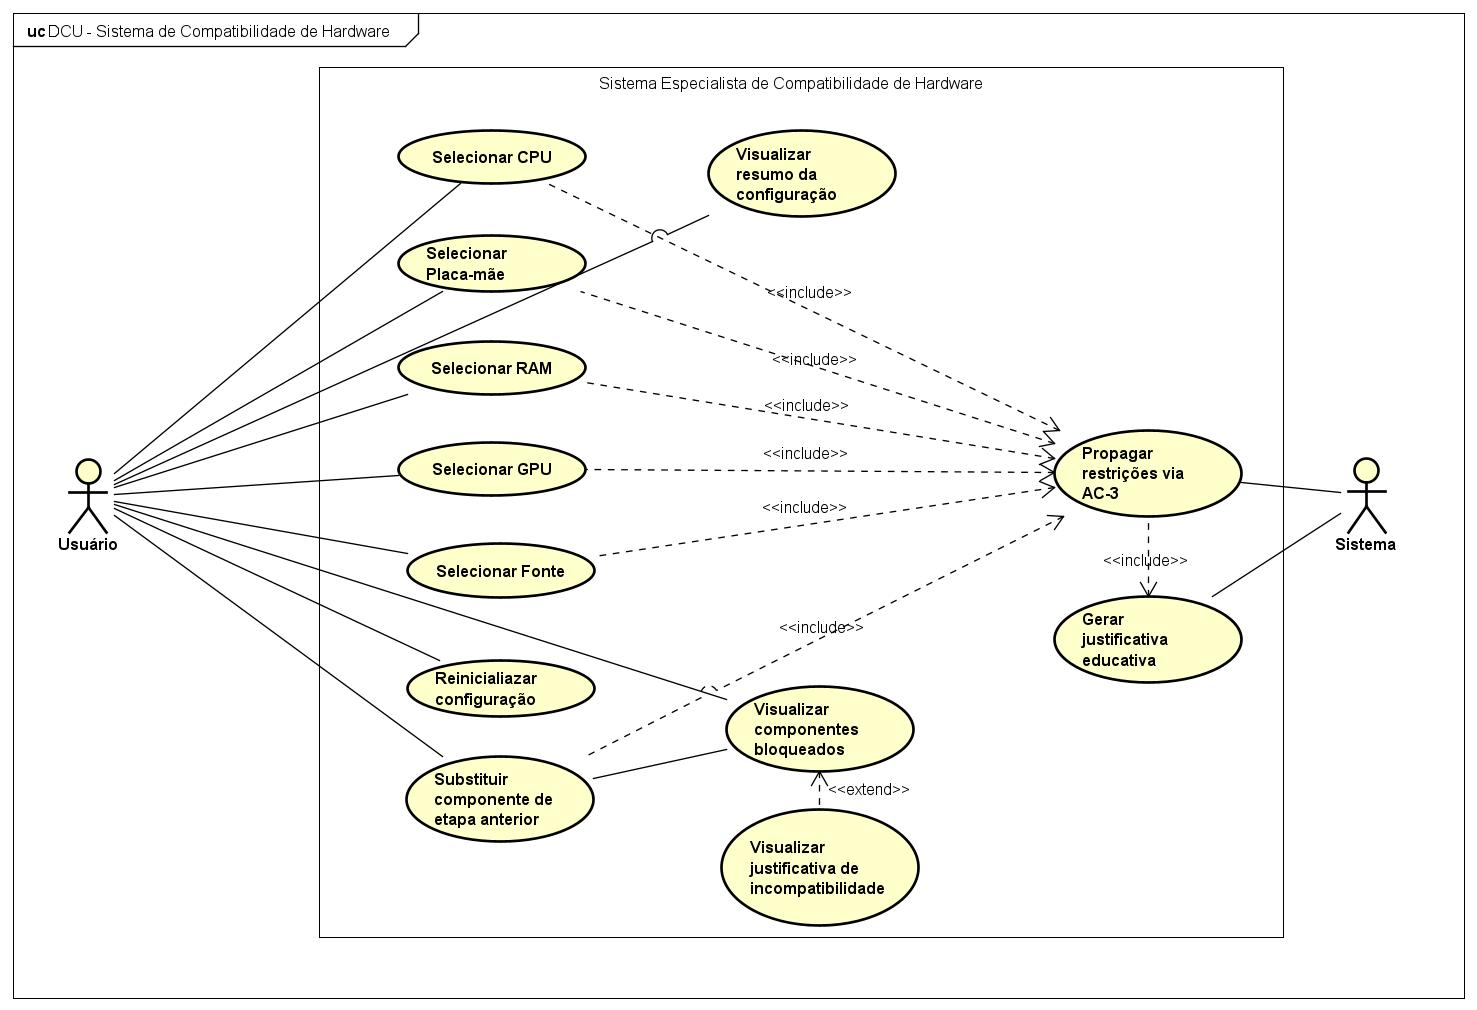
\includegraphics[width=1\textwidth]{imagens/DCU - Sistema de Compatibilidade de Hardware.jpg}
  \\\textbf{Fonte:} Elaborada pelo autor
  \label{fig:diagCasosDeUso}
\end{figure}
\FloatBarrier

\subsection{Especificação dos Casos de Uso}

Uma especificação de caso de uso fornece detalhe textual para um caso de uso.
A Tabela~\ref{tab:especCasosDeUso} apresenta o modelo de estrutura de tópicos
adotado para a especificação dos casos de uso deste trabalho (extraído de
\href{https://www.ibm.com/docs/pt-br/elm/6.0?topic=cases-use-case-specification-outline}{IBM-Especificação de Casos de Uso}).

\FloatBarrier
\begin{table}[!htbp]
  \centering
  \caption{Modelo para Especificação de Casos de Uso}
  \begin{tabular}{ c | p{11.5cm} }
    \hline
    \textbf{Item}        & \textbf{Descrição}                                                                                                                                                                                                                                                                                                                                                                                                                                                                                            \\ \hline
    Nome do Caso de Uso  &
    Declara o nome do caso de uso. Geralmente, o nome expressa o objetivo ou resultado observável do caso de uso, como ``Sacar Dinheiro'' no caso de um caixa eletrônico.                                                                                                                                                                                                                                                                                                                                                                \\ \hline
    Descrição Resumida   & Descreve a função e o objetivo do caso de uso.                                                                                                                                                                                                                                                                                                                                                                                                                                                                \\ \hline
    Fluxo de Eventos     & Apresenta o fluxo básico e os fluxos alternativos. O fluxo de eventos descreve o comportamento do sistema; ele não descreve como o sistema funciona, os detalhes da apresentação ou os detalhes da interface com o usuário. Se forem trocadas informações, o caso de uso deverá ser específico sobre o que será transmitido de um lado para outro. Por exemplo, em vez de descrever uma ação como ``o agente insere informações do cliente'', indique que ``o agente insere o nome e o endereço do cliente''. \\ \hline
    Fluxo Básico         & Descreve o comportamento principal ideal do sistema.                                                                                                                                                                                                                                                                                                                                                                                                                                                          \\ \hline
    Fluxos Alternativos  & Descreve exceções ou desvios do fluxo básico, como o comportamento do sistema quando o agente insere um ID de usuário incorreto e a autenticação do usuário falha.                                                                                                                                                                                                                                                                                                                                            \\ \hline
    Requisitos Especiais & Requisitos não-funcionais que são específicos para um caso de uso mas que não são especificados no texto do fluxo do caso de uso de eventos. Exemplos de requisitos especiais incluem estes fatores: requisitos legais e regulamentares; padrões de aplicativo; atributos de qualidade do sistema, incluindo usabilidade, confiabilidade, desempenho e capacidade de suporte; sistemas operacionais e ambientes; requisitos de compatibilidade e restrições de design.                                        \\ \hline
    Condições Prévias    & Um estado do sistema que deve estar presente antes de um caso de uso ser iniciado.                                                                                                                                                                                                                                                                                                                                                                                                                            \\ \hline
    Pós-Condições        & Uma lista de estados possíveis para o sistema imediatamente após a conclusão de um caso de uso.                                                                                                                                                                                                                                                                                                                                                                                                               \\ \hline
    Pontos de Extensão   & Um ponto no fluxo de eventos do caso de uso em que outro caso de uso é referenciado.                                                                                                                                                                                                                                                                                                                                                                                                                          \\ \hline
  \end{tabular}
  \\ \vspace{0.2cm}
  \textbf{Fonte:} Extraído de \href{https://www.ibm.com/docs/pt-br/elm/6.0?topic=cases-use-case-specification-outline}{IBM-Especificação de Casos de Uso}
  \label{tab:especCasosDeUso}
\end{table}
\FloatBarrier

A título de exemplo, a Tabela~\ref{tab:ucSelecionarComponente} apresenta a
especificação do caso de uso \textit{Selecionar Componente}, central ao fluxo de
configuração do sistema.

\FloatBarrier
\begin{table}[!htbp]
  \centering
  \caption{Especificação do Caso de Uso ``Selecionar Componente''}
  \begin{tabular}{ | p{15cm} | }
    \hline
    \textbf{Caso de Uso}                                                                                                                                                                                                                   \\
    Selecionar Componente                                                                                                                                                                                                                  \\	\hline
    \textbf{Referências}                                                                                                                                                                                                                   \\
    RF-01, RF-05, RF-09, RF-10                                                                                                                                                                                                             \\	\hline
    \textbf{Descrição Geral}                                                                                                                                                                                                               \\
    O caso de uso inicia-se quando o usuário seleciona um componente em uma das etapas do \textit{wizard} de configuração. O sistema dispara a propagação de restrições e atualiza a disponibilidade dos componentes nas etapas seguintes. \\	\hline
    \textbf{Atores}                                                                                                                                                                                                                        \\
    Usuário, Sistema                                                                                                                                                                                                                       \\	\hline
    \textbf{Pré-Condições}                                                                                                                                                                                                                 \\
    A base de conhecimento deve estar populada; o usuário deve estar em uma etapa válida do \textit{wizard}.                                                                                                                               \\	\hline
    \textbf{Garantia de Sucesso (Pós-Condições)}                                                                                                                                                                                           \\
    Componente registrado na configuração; domínios das categorias seguintes atualizados; componentes incompatíveis sinalizados com a respectiva justificativa.                                                                            \\	\hline
    \textbf{Requisitos Especiais}                                                                                                                                                                                                          \\
    A propagação deve ocorrer em tempo real (RNF-01); nenhum bloqueio pode ocorrer sem justificativa (RNF-14).                                                                                                                             \\	\hline
    \textbf{Fluxo Básico}
    \begin{enumerate}
      \item Usuário visualiza a lista de componentes da categoria atual;
      \item Usuário seleciona um componente compatível;
      \item Sistema registra a seleção e envia o estado completo à API REST;
      \item Sistema executa o algoritmo AC-3 sobre o grafo de restrições;
      \item Sistema poda os domínios das categorias seguintes e retorna os componentes disponíveis;
      \item Sistema apresenta a etapa seguinte com os componentes atualizados.
    \end{enumerate}
    \\	\hline
    \textbf{Fluxo Alternativo}
    \renewcommand{\labelenumii}{\arabic{enumi}.\arabic{enumii}}
    \begin{enumerate}
      \item Usuário tenta selecionar um componente incompatível
            \begin{enumerate}
              \item Sistema bloqueia a seleção e exibe a justificativa técnica da incompatibilidade (RF-10);
              \item Retorna ao passo 1.
            \end{enumerate}
    \end{enumerate}
    \\	\hline
  \end{tabular}
  \label{tab:ucSelecionarComponente}
\end{table}
\FloatBarrier

\section{Modelo de Domínio}

O modelo de domínio é um artefato de análise que representa os conceitos
relevantes do domínio do problema e os relacionamentos entre eles, sem
preocupação com detalhes de implementação \cite{larman2004}. Por se concentrar
no vocabulário do domínio, o modelo é elaborado apenas com as classes e seus
atributos, auxiliando na compreensão da aplicação. A
Figura~\ref{fig:modeloDeDominio} apresenta o modelo de domínio desenvolvido
neste trabalho.

O modelo reflete a decisão arquitetural de tornar a tripla $\langle X, D, C
  \rangle$ do CSP configurável. Em vez de especializar a classe \textit{Componente}
em subclasses fixas (CPU, Placa-mãe, RAM, GPU e Fonte), com atributos codificados,
adota-se uma estrutura genérica baseada em metadados: a classe \textit{Categoria}
representa as variáveis ($X$); a classe \textit{Componente} representa os valores
de domínio ($D$); a classe \textit{Caracteristica} define, por categoria, os
atributos configuráveis, cujos valores são registrados em
\textit{ComponenteCaracteristica}; e a classe \textit{Restricao} representa o
conjunto $C$, associando duas características por meio de um operador. Essa
organização realiza concretamente os requisitos RNF-07 e RNF-08, uma vez que a
inclusão de novas categorias, características ou restrições não exige alteração de
código, apenas a inserção de novos registros na base de conhecimento.

\FloatBarrier
\begin{figure}[!htbp]
  \centering
  \caption{Modelo de Domínio}
  %scale redimensiona a figura.
  %1.5 = 150% do tamanho original
  %1 = 100% do tamanho original
  %0.20 = 20% do tamanho original
  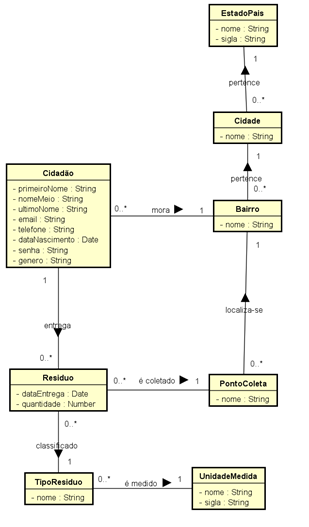
\includegraphics[width=1\textwidth]{imagens/ModelodeDominio.png}
  \\\textbf{Fonte:} Elaborada pelo autor
  \label{fig:modeloDeDominio}
\end{figure}
\FloatBarrier

% \section{Diagrama de Objetos}
% Fazer uma pequena definição de diagrama de objetos para introduzir essa seção. Terminar o parágrafo informando qual figura apresenta o diagrama de objetos. Elabore o diagrama de objetos para cada classe identificada no modelo de domínio.


\section{Diagrama de Classes de Análise}

O diagrama de classes de análise é uma evolução do modelo de domínio que
incorpora, além dos atributos, os métodos que descrevem o comportamento das
classes, aproximando o modelo da estrutura que será implementada
\cite{larman2004}. A Figura~\ref{fig:classesDeAnalise} apresenta o diagrama de
classes de análise elaborado neste trabalho.

Em relação ao modelo de domínio, o diagrama acrescenta os métodos responsáveis
pela lógica do sistema. A classe \textit{Restricao} recebe o método
\textit{isSatisfeita}, que avalia se os valores de duas características atendem ao
operador definido; a classe \textit{ComponenteCaracteristica} expõe o método de
acesso ao valor; e são introduzidas as classes de saída do motor de inferência,
\textit{ResultadoValidacao} e \textit{JustificativaEducativa}, responsáveis por
transportar, respectivamente, o resultado da propagação e as justificativas
educativas exibidas ao usuário. Diferentemente das classes da base de
conhecimento, essas duas classes não são persistidas, sendo geradas a cada
execução do AC-3.

\FloatBarrier
\begin{figure}[!htbp]
  \centering
  \caption{Diagrama de Classes de Análise}
  %scale redimensiona a figura.
  %1.5 = 150% do tamanho original
  %1 = 100% do tamanho original
  %0.20 = 20% do tamanho original
  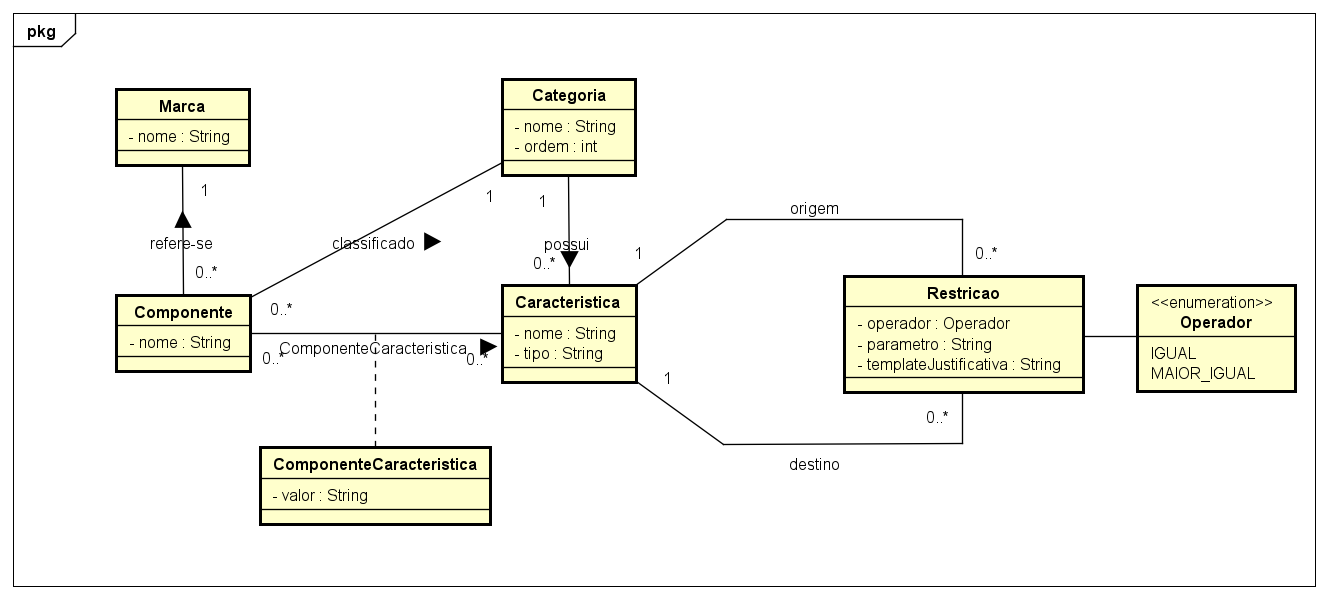
\includegraphics[width=1\textwidth]{imagens/diagrama-classe-v2.png}
  \\\textbf{Fonte:} Elaborada pelo autor
  \label{fig:classesDeAnalise}
\end{figure}
\FloatBarrier

\section{Diagrama de Atividades}

Um diagrama de atividades ilustra a natureza dinâmica de um sistema pela
modelagem do fluxo de controle de uma atividade à outra. Uma atividade
representa uma operação em alguma classe do sistema que resulta em uma mudança de
estado. Tipicamente, diagramas de atividades são usados para modelar fluxos de
processos, processos de negócios ou operações internas. Embora seja semelhante a
uma máquina de estados, o diagrama de atividades tem propósito distinto, voltado
a capturar ações e seus resultados em termos de mudanças no estado do objeto.

O fluxo é mostrado por meio de transições, representadas por setas direcionadas
que indicam o caminho entre os estados de atividade (ação). Um diagrama de
atividades é normalmente composto pelos seguintes elementos: atividades (ações),
estados de atividade (ação), transição, fluxo de objeto, estado inicial, estado
final, \textit{branching}, sincronização e raias.

% \FloatBarrier
% \begin{figure}[!htbp]
%   \centering
%   \caption{Diagrama de Atividades}
%   \includegraphics[width=1\textwidth]{imagens/Diagrama de Atividades.png}
%   \\\textbf{Fonte:} Elaborada pelo autor
%   \label{fig:diagramaDeAtividades}
% \end{figure}
% \FloatBarrier
\input{capitulo06ProjetodeSoftware}
\chapter{Implementação}
\label{cap:07}

Este capítulo descreve a concretização do sistema especialista educacional cujos requisitos e projeto foram apresentados nos Capítulos~\ref{cap:05} e~\ref{cap:06}. Mais do que relatar quais tecnologias foram empregadas, busca-se justificar as decisões de implementação que sustentam as propriedades centrais do trabalho: a generalidade do motor de inferência, seu determinismo e sua capacidade de explicação. São detalhados o ambiente e as ferramentas de desenvolvimento, a organização do repositório e a implementação de cada uma das três camadas arquiteturais, bem como a interface de comunicação entre elas. Dá-se ênfase à camada de lógica de negócio, que abriga o motor de inferência AC-3 e a \textit{explanation facility}, por constituírem o núcleo da contribuição deste trabalho. Ao final, registram-se as limitações conhecidas da implementação em seu estado atual.

% ============================================================
\section{Ambiente e Ferramentas de Desenvolvimento}
\label{sec:ambiente-implementacao}
% ============================================================

A escolha das tecnologias foi orientada por um princípio unificador: adotar um único ecossistema de linguagem em todas as camadas, de modo a permitir o compartilhamento de definições de tipos entre o servidor e o cliente. Por essa razão, o sistema foi desenvolvido integralmente em \textit{TypeScript}~\cite{TypeScript}, cuja tipagem estática permite que os contratos de dados trafegados entre as camadas sejam verificados em tempo de compilação, reduzindo a classe de erros que só se manifestaria em execução. O ambiente de execução do lado do servidor é o \textit{Node.js}~\cite{NodeJS}, escolhido justamente por executar TypeScript no servidor e, assim, viabilizar esse ecossistema unificado.

A camada de dados é provida pelo \textit{PostgreSQL}~\cite{PostgreSQL} em sua versão 16, selecionado por sua robustez, conformidade com o padrão SQL e adequação ao modelo relacional exigido pela base de conhecimento. Sua execução em contêiner por meio do \textit{Docker}~\cite{Docker} foi uma decisão deliberada para garantir um ambiente de banco de dados reprodutível e idêntico entre as máquinas de desenvolvimento, atendendo diretamente ao requisito RNF-12 e dispensando a instalação manual do banco no sistema operacional. Durante o desenvolvimento, a inspeção e a manipulação manual dos dados foram realizadas com o \textit{DBeaver}~\cite{DBeaver}, e a codificação foi conduzida no \textit{Visual Studio Code}~\cite{VSCode}. O Quadro~\ref{qua:versoes} consolida as versões das principais tecnologias empregadas.

\FloatBarrier
\begin{quadro}[!htbp]
  \centering
  \caption{Versões das principais tecnologias utilizadas}
  \begin{tabular}{l l}
    \hline
    \textbf{Tecnologia} & \textbf{Versão} \\ \hline
    Node.js             & $\geq$ 20.0.0   \\ \hline
    TypeScript          & 5.6.3           \\ \hline
    NestJS              & 10.4.15         \\ \hline
    Next.js             & 15.1.3          \\ \hline
    React               & 19.0.0          \\ \hline
    Prisma ORM          & 5.22.0          \\ \hline
    PostgreSQL          & 16              \\ \hline
    pnpm                & 9.15.0          \\ \hline
    Turborepo           & 2.3.3           \\ \hline
  \end{tabular}
  \\ \vspace{0.2cm}
  \textbf{Fonte:} Elaborada pelo autor
  \label{qua:versoes}
\end{quadro}
\FloatBarrier

% ============================================================
\section{Organização do Repositório}
\label{sec:monorepo}
% ============================================================

O código-fonte foi organizado como um \textit{monorepo}, isto é, um único repositório que abriga múltiplos projetos relacionados, gerenciado pelo \textit{pnpm}~\cite{Pnpm} como gerenciador de pacotes e pelo \textit{Turborepo}~\cite{Turborepo} como orquestrador das tarefas de \textit{build} e execução. A opção pelo monorepo, em vez de repositórios separados para servidor e cliente, decorre diretamente da estratégia de ecossistema unificado: mantendo ambos no mesmo repositório, torna-se possível extrair as definições de tipos compartilhadas para um pacote interno, consumido tanto pelo servidor quanto pelo cliente. Assim, o contrato de comunicação entre as camadas existe em um único lugar, e qualquer alteração é verificada em tempo de compilação em ambos os lados, eliminando a duplicação e a divergência silenciosa de tipos que ocorreria com repositórios independentes.

O repositório organiza-se em dois diretórios principais. O diretório \texttt{apps} contém as aplicações executáveis: \texttt{api}, que implementa as camadas de lógica de negócio e de dados em NestJS~\cite{NestJS}, e \texttt{web}, que implementa a camada de apresentação em Next.js~\cite{NextJS}. O diretório \texttt{packages} contém os módulos compartilhados, com destaque para \texttt{shared-types}, que centraliza as interfaces trafegadas entre cliente e servidor, como \texttt{EstadoConfiguracao}, \texttt{RespostaValidacao} e \texttt{JustificativaEducativa}. A estrutura simplificada do repositório é apresentada no Código~\ref{lst:monorepo}.

\begin{lstlisting}[caption={Estrutura simplificada do monorepo},label={lst:monorepo},basicstyle=\ttfamily\small]
apps/
  api/
    prisma/        (schema.prisma, migrations/, seed.ts)
    src/
      app.module.ts, main.ts
      categorias/   components/   configurations/
      csp/          explanations/  prisma/
  web/
    src/
      app/          (layout.tsx, page.tsx, wizard/page.tsx)
      components/   (ui/)
      lib/          (api.ts, utils.ts)
packages/
  shared-types/     (src/index.ts)
  tsconfig/         (base.json, nestjs.json, nextjs.json)
\end{lstlisting}
\fonte{Elaborado pelo autor}

Essa organização não é meramente estética: ela materializa fisicamente a separação estrita entre as três camadas exigida pelo requisito RNF-06. A camada de dados reside nos módulos \texttt{prisma} e \texttt{csp} do lado do servidor, a lógica de negócio nos módulos \texttt{csp}, \texttt{configurations} e \texttt{explanations}, e a apresentação integralmente no aplicativo \texttt{web}. O pacote \texttt{shared-types} não contém lógica de execução, apenas contratos, funcionando como uma fronteira tipada explícita entre as camadas distribuídas de modo que a comunicação entre elas é obrigada a passar por um contrato conhecido, e não por acoplamento direto.

% ============================================================
\section{Camada de Dados}
\label{sec:impl-dados}
% ============================================================

A persistência foi implementada sobre o PostgreSQL, acessado a partir da camada de lógica de negócio por intermédio do \textit{Prisma ORM}~\cite{Prisma}, responsável por mapear os registros relacionais em objetos da aplicação. A adoção de um ORM justifica-se por manter a camada de lógica de negócio trabalhando com objetos tipados, sem consultas SQL escritas manualmente, o que preserva a coerência com o ecossistema TypeScript e reduz a superfície de erro no acesso a dados. O esquema do banco reproduz fielmente o modelo genérico baseado no padrão Entidade-Atributo-Valor (EAV) apresentado na Seção~\ref{sec:projetoDados} do Capítulo~\ref{cap:06}, materializando as seis relações \texttt{Marca}, \texttt{Categoria}, \texttt{Caracteristica}, \texttt{Componente}, \texttt{ComponenteCaracteristica} e \texttt{Restricao}, além dos dois tipos enumerados \texttt{TipoCaracteristica} (\texttt{TEXTO}, \texttt{INTEIRO}) e \texttt{OperadorRestricao} (\texttt{IGUAL}, \texttt{MAIOR\_OU\_IGUAL}).

A decisão de projeto mais consequente desta camada é a representação das restrições como dados, e não como código. O Código~\ref{lst:schema-restricao} apresenta a definição da entidade \texttt{Restricao} no \textit{schema} do Prisma, elemento central do modelo por representar cada aresta do grafo de restrições, ou seja, cada elemento do conjunto $C$ do CSP.

\begin{lstlisting}[caption={Definição da entidade Restricao no schema do Prisma},label={lst:schema-restricao},basicstyle=\ttfamily\small]
model Restricao {
  id                    String            @id @default(uuid())
  idCaracteristica1     String
  idCaracteristica2     String
  operador              OperadorRestricao
  parametro             String?
  templateJustificativa String

  caracteristica1 Caracteristica @relation("origem",  ...)
  caracteristica2 Caracteristica @relation("destino", ...)
}
\end{lstlisting}
\fonte{Elaborado pelo autor}

Ao guardar em cada registro as duas características relacionadas, o operador e o texto da justificativa, uma restrição passa a ser inteiramente descrita por uma linha da tabela. Essa escolha é o que sustenta a expansibilidade exigida pelos requisitos RNF-07 e RNF-08: incluir uma nova restrição, ou mesmo uma nova categoria de componente, reduz-se a inserir registros, sem qualquer alteração no motor de inferência. É essa decisão que concretiza, no nível da persistência, a ambição de um motor genérico e reutilizável.

A gestão do esquema é feita por meio das \textit{migrations} do Prisma, aplicadas com o comando \texttt{prisma migrate dev}, o que mantém a evolução do banco versionada e reproduzível. Duas \textit{migrations} compõem o histórico do projeto: a criação inicial do esquema e a subsequente adoção do modelo EAV genérico, transição que reflete, no próprio versionamento, a decisão de abandonar tabelas específicas por categoria em favor da estrutura genérica. A carga inicial da base de conhecimento é realizada por um procedimento de \textit{Database Seeding} (\texttt{seed.ts}), em conformidade com o requisito RF-18. O Quadro~\ref{qua:seed} apresenta a contagem de registros inseridos pela carga inicial, dimensionada para cobrir as plataformas AMD AM4 e AM5 e, com isso, viabilizar os cenários de validação previstos.

\FloatBarrier
\begin{quadro}[!htbp]
  \centering
  \caption{Registros criados pela carga inicial da base de conhecimento}
  \begin{tabular}{l c}
    \hline
    \textbf{Entidade}        & \textbf{Registros} \\ \hline
    Marca                    & 5                  \\ \hline
    Categoria                & 5                  \\ \hline
    Caracteristica           & 19                 \\ \hline
    Componente               & 11                 \\ \hline
    ComponenteCaracteristica & 40                 \\ \hline
    Restricao                & 4                  \\ \hline
  \end{tabular}
  \\ \vspace{0.2cm}
  \textbf{Fonte:} Elaborada pelo autor
  \label{qua:seed}
\end{quadro}
\FloatBarrier

As quatro restrições cadastradas correspondem exatamente às arestas do grafo definido no Capítulo~\ref{cap:02}: soquete entre CPU e placa-mãe, padrão de memória entre placa-mãe e RAM, e capacidade energética da fonte em relação ao TDP da CPU e ao TDP da GPU, respectivamente.

% ============================================================
\section{Camada de Lógica de Negócio}
\label{sec:impl-logica}
% ============================================================

A camada de lógica de negócio é o núcleo inteligente do sistema e concentra a contribuição técnica deste trabalho. Foi implementada em NestJS, \textit{framework} escolhido por organizar a aplicação em módulos, \textit{controllers} e \textit{services}, estrutura que favorece a separação de responsabilidades e alinha-se diretamente aos princípios da arquitetura em camadas discutidos no Capítulo~\ref{cap:02}. Esta seção detalha, de dentro para fora, o isolamento do motor, a montagem do grafo de restrições, o algoritmo AC-3, o avaliador genérico de restrições e a geração das justificativas educativas.

\subsection{Isolamento do Motor de Inferência}
\label{sub:isolamento-motor}
A decisão de projeto mais importante desta camada foi manter o motor de inferência inteiramente independente do \textit{framework} e do mecanismo de persistência. Os arquivos que implementam o algoritmo AC-3 (\texttt{ac3.ts}) e a avaliação de restrições (\texttt{constraint-evaluator.ts}) não importam qualquer artefato do NestJS ou do Prisma, não contêm decoradores nem efeitos colaterais de entrada e saída, operando como funções puras sobre estruturas de dados recebidas por parâmetro.

Esse isolamento não é um detalhe de organização, mas o que garante três propriedades fundamentais do trabalho. Primeiro, o determinismo (RNF-10): sem qualquer dependência de estado externo ou de operações de entrada e saída, a mesma entrada produz invariavelmente a mesma saída. Segundo, a testabilidade: por não depender do \textit{framework}, o motor pode ser exercitado por testes unitários que não exigem servidor nem banco de dados em execução. Terceiro, e mais importante para a tese central deste trabalho, a agnosticidade ao domínio: o motor não conhece o conceito de \textit{hardware}, de soquete ou de TDP, opera exclusivamente sobre variáveis, domínios e restrições. Todo o conhecimento específico do domínio reside nos dados, e não no algoritmo, o que torna o motor, em princípio, aplicável a qualquer problema de configuração modelável como CSP.

\subsection{Carregamento e Montagem do Grafo}
\label{sub:montagem-grafo}
A validação inicia-se no \texttt{CspService}, que, a cada requisição, carrega as restrições persistidas e as converte em uma representação interna independente do banco. Essa reconstrução a cada chamada é uma consequência direta da decisão de projeto pela ausência de estado no servidor: em conformidade com o princípio \textit{stateless} (RNF-11), nenhuma informação de sessão é mantida entre requisições, e o grafo é montado a partir da base de conhecimento sempre que uma validação é solicitada. O Código~\ref{lst:carregar-restricoes} apresenta esse carregamento, no qual cada linha da tabela \texttt{Restricao} é mapeada para a estrutura interna \texttt{RestricaoInterna}, resolvendo, por meio das características associadas, quais categorias, as variáveis do CSP, a restrição conecta.

\begin{lstlisting}[caption={Carregamento das restrições a partir da base de conhecimento},label={lst:carregar-restricoes},basicstyle=\ttfamily\small]
private async carregarRestricoes(): Promise<RestricaoInterna[]> {
  const linhas = await this.prisma.restricao.findMany({
    include: {
      caracteristica1: { select: { categoriaId: true } },
      caracteristica2: { select: { categoriaId: true } },
    },
  });

  return linhas.map((linha) => ({
    id:                linha.id,
    variavelDemanda:   linha.caracteristica1.categoriaId,
    variavelCapacidade:linha.caracteristica2.categoriaId,
    caracteristica1Id: linha.caracteristica1Id,
    caracteristica2Id: linha.caracteristica2Id,
    operador:          linha.operador,
    parametro:         linha.parametro ?? undefined,
    templateJustificativa: linha.templateJustificativa,
  }));
}
\end{lstlisting}
\fonte{Elaborado pelo autor}

Cada variável do CSP é representada por uma estrutura que associa a categoria ao seu domínio, mantido em um \texttt{Map} de componentes. A escolha do \texttt{Map} deve-se à necessidade de remover valores do domínio de forma eficiente durante a propagação, operação frequente no AC-3. Sobre o conjunto de restrições, o motor constrói uma \textbf{lista de adjacência}, conforme justificado teoricamente no Capítulo~\ref{cap:02} como a representação mais adequada para grafos esparsos. A lista é materializada uma única vez no início da execução, indexando, para cada variável, os arcos direcionados que a alcançam, como mostra o Código~\ref{lst:lista-adjacencia}.

\begin{lstlisting}[caption={Construção da lista de adjacência do grafo de restrições},label={lst:lista-adjacencia},basicstyle=\ttfamily\small]
function construirListaAdjacencia(
  restricoes: RestricaoInterna[],
): Map<string, Arco[]> {
  const mapa = new Map<string, Arco[]>();
  const adicionar = (chave: string, arco: Arco) => {
    const lista = mapa.get(chave);
    if (lista) lista.push(arco);
    else mapa.set(chave, [arco]);
  };

  for (const r of restricoes) {
    adicionar(r.variavelDemanda,
      { origem: r.variavelCapacidade, destino: r.variavelDemanda, restricao: r });
    if (r.variavelDemanda !== r.variavelCapacidade) {
      adicionar(r.variavelCapacidade,
        { origem: r.variavelDemanda, destino: r.variavelCapacidade, restricao: r });
    }
  }
  return mapa;
}
\end{lstlisting}
\fonte{Elaborado pelo autor}

A opção pela lista de adjacência indexada, em vez de percorrer o conjunto completo de restrições a cada consulta, alinha a implementação à fundamentação teórica e assegura que a recuperação dos vizinhos de uma variável ocorra em tempo proporcional ao seu grau. Como cada restrição binária origina dois arcos direcionados, a lista preserva a orientação exigida pelo algoritmo, distinção necessária porque, no motor, a direção do arco determina qual característica é tratada como demanda e qual como capacidade.

\subsection{O Algoritmo AC-3}
\label{sub:impl-ac3}
O motor implementa o algoritmo AC-3 conforme descrito por~\textcite{Mackworth1977} e~\textcite{Russell2010}, decisão fundamentada no Capítulo~\ref{cap:02}: por operar por propagação de restrições, e não por enumeração exaustiva, o AC-3 evita a explosão combinatória que inviabilizaria a validação por força bruta (RNF-02). Uma fila é inicializada com todos os arcos direcionados; a cada iteração, um arco é retirado e submetido ao procedimento de revisão, que remove do domínio da variável de origem os valores sem suporte na variável de destino. Sempre que ocorre uma remoção, os arcos que incidem sobre a variável afetada são reinseridos na fila, propagando a mudança pela rede até o ponto de estabilidade. O Código~\ref{lst:revisar} apresenta esse procedimento de revisão.

\begin{lstlisting}[caption={Procedimento de revisão de arco do algoritmo AC-3},label={lst:revisar},basicstyle=\ttfamily\small]
function revisar(arco: Arco, variaveis: VariavelCSP[]): ValorRemovido[] {
  const removidos: ValorRemovido[] = [];
  const varOrigem  = getVariavel(variaveis, arco.origem);
  const varDestino = getVariavel(variaveis, arco.destino);
  if (!varOrigem || !varDestino) return removidos;

  const arcoReverso   = arco.origem === arco.restricao.variavelCapacidade;
  const valoresDestino = Array.from(varDestino.dominio.values());
  if (valoresDestino.length === 0) return removidos;

  for (const v of Array.from(varOrigem.dominio.values())) {
    const temSuporte = valoresDestino.some((w) =>
      arcoReverso
        ? avaliarRestricao(w, v, arco.restricao)
        : avaliarRestricao(v, w, arco.restricao),
    );
    if (!temSuporte) {
      varOrigem.dominio.delete(v.id);
      removidos.push({
        categoriaId:     varOrigem.categoriaId,
        componenteId:    v.id,
        componente:      v,
        restricaoViolada: arco.restricao,
        ancora:          valoresDestino[0],
      });
    }
  }
  return removidos;
}
\end{lstlisting}
\fonte{Elaborado pelo autor}

Um aspecto de projeto merece destaque: cada valor removido não é simplesmente descartado, mas registrado em uma estrutura \texttt{ValorRemovido} que retém a restrição violada e um componente-âncora, o valor da variável vizinha que fundamenta o bloqueio. Essa decisão é o que torna possível, mais adiante, rastrear cada bloqueio até a restrição que o originou (RNF-13) e produzir a justificativa educativa correspondente, assegurando que nenhum bloqueio ocorra silenciosamente (RNF-14). Em outras palavras, a \textit{explanation facility} não é um acréscimo posterior ao motor: a informação necessária para explicar é coletada no exato instante da poda.

\subsection{Avaliação Genérica de Restrições}
\label{sub:impl-avaliador}
O suporte entre dois valores é decidido pela função \texttt{avaliarRestricao}, apresentada no Código~\ref{lst:avaliar}, que aplica o operador definido na própria restrição, sem qualquer ramificação por tipo de característica ou de componente.

\begin{lstlisting}[caption={Avaliação genérica de uma restrição},label={lst:avaliar},basicstyle=\ttfamily\small]
export function avaliarRestricao(
  valorVar1: Componente,
  valorVar2: Componente,
  restricao: RestricaoInterna,
): boolean {
  const val1 = getValor(valorVar1, restricao.caracteristica1Id);
  const val2 = getValor(valorVar2, restricao.caracteristica2Id);
  if (val1 === undefined || val2 === undefined) return true;

  if (restricao.operador === 'IGUAL') {
    return val1 === val2;
  }
  const parametro = Number(restricao.parametro ?? '1');
  return Number(val2) >= Number(val1) * parametro;
}
\end{lstlisting}
\fonte{Elaborado pelo autor}

A ausência deliberada de qualquer condicional específica por domínio é o que concretiza, no nível do algoritmo, os requisitos RNF-07 e RNF-08: o mesmo código avalia a compatibilidade de soquete, o padrão de memória ou a capacidade energética, distinguindo esses casos apenas pelo operador e pelas características cadastradas na base de conhecimento. O operador \texttt{IGUAL} implementa as restrições binárias absolutas de soquete e de padrão de memória; o operador \texttt{MAIOR\_OU\_IGUAL} implementa a restrição quantitativa de capacidade energética, na qual o parâmetro cadastrado, por exemplo, $1{,}25$, representa a margem de segurança aplicada sobre a demanda. Cada verificação de potência é realizada entre um par de variáveis, decisão que preserva a natureza estritamente binária do grafo de restrições; as implicações dessa modelagem são discutidas na Seção~\ref{sec:impl-limitacoes}.

O sobredimensionamento da fonte em relação ao consumo calculado constitui prática
recomendada pelos fabricantes, que incorporam reserva de potência às próprias ferramentas
de dimensionamento, destinada a cobrir picos de carga, eventual substituição de componentes
e a estabilidade da operação \cite{SEASONIC2026}. O valor de 25\% adotado neste trabalho
foi definido de forma arbitrária e não deriva de norma técnica. Cabe observar que tal valor
não se encontra codificado no motor de inferência, mas cadastrado como parâmetro da própria
restrição na base de conhecimento, de modo que o sistema admite qualquer fator de acréscimo
sem alteração do algoritmo. Essa característica reforça os requisitos de expansibilidade
estabelecidos, uma vez que o ajuste da margem depende apenas da atualização de um registro.

\subsection{Geração das Justificativas Educativas}
\label{sub:impl-explicacoes}
A \textit{explanation facility}, característica que distingue o sistema de um mero mecanismo de filtragem, é implementada no \texttt{ExplanationsService}. Para cada valor removido pelo AC-3, o serviço formula uma justificativa em linguagem natural a partir do \texttt{templateJustificativa} associado à restrição violada, substituindo marcadores por valores concretos dos componentes envolvidos. Os marcadores suportados são \texttt{\{comp1.nome\}}, \texttt{\{val1\}}, \texttt{\{comp2.nome\}}, \texttt{\{val2\}} e \texttt{\{val1\_com\_margem\}}, este último aplicável às restrições quantitativas, no qual o consumo é apresentado já acrescido da margem de segurança.

A decisão de manter o texto de cada explicação inteiramente no dado cadastrado, e não no código, é coerente com toda a arquitetura genérica adotada: assim como nenhuma regra de compatibilidade está embutida no motor, nenhum termo técnico do domínio está embutido no serviço de explicações. Toda a dimensão educativa emerge da base de conhecimento. Como consequência, ao bloquear um módulo DDR4 diante de uma placa-mãe que suporta exclusivamente DDR5, o sistema não apenas remove a opção, mas comunica a regra física violada em linguagem acessível, transformando o bloqueio em oportunidade de aprendizagem (RF-10 a RF-13), que é precisamente o objetivo educacional do trabalho.

% ============================================================
\section{Camada de Apresentação}
\label{sec:impl-apresentacao}
% ============================================================

A camada de apresentação foi implementada em Next.js, utilizando o \textit{App Router} e a biblioteca React~\cite{ReactJS} em sua versão 19. A interface adota o formato \textit{wizard}, conduzindo o usuário sequencialmente pelas cinco categorias de componentes, decisão de projeto que reduz a carga cognitiva do usuário leigo ao decompor a montagem em etapas discretas. O estado da configuração, etapa atual, seleções realizadas e resultado da última validação, é mantido no próprio cliente por meio do mecanismo de estado do React, sem persistência no servidor, opção coerente com o caráter \textit{stateless} da API e com o requisito RNF-05, que dispensa cadastro ou autenticação.

A comunicação com a camada de lógica de negócio é encapsulada em um módulo cliente (\texttt{lib/api.ts}) que expõe as operações de listagem de categorias, listagem de componentes e validação da configuração. Esse encapsulamento concentra em um único ponto o conhecimento sobre como falar com o servidor, isolando o restante da interface dos detalhes de comunicação. A cada alteração de seleção, a interface envia o estado completo à API e recebe, em resposta, os domínios atualizados e as justificativas dos bloqueios, atualizando a exibição em tempo real.

A decisão de interface mais alinhada ao objetivo educativo é a de não ocultar os componentes incompatíveis. Em vez de removê-los da listagem, comportamento típico dos mecanismos de filtragem, eles permanecem visíveis, com sinalização visual de bloqueio, e a justificativa técnica correspondente é revelada quando o usuário interage com o componente, atendendo aos requisitos RF-03 e RNF-14. Ao término da seleção de todas as categorias, a interface apresenta a tela de resumo, que consolida a configuração montada, exibe seu status geral de compatibilidade e o consumo energético estimado, e registra o tempo de execução da validação.

Para tornar concreto o encadeamento entre as camadas, convém percorrer o fluxo completo de uma interação. Quando o usuário seleciona um componente, a interface registra a escolha no estado local e envia o estado completo das seleções à API. No servidor, o \texttt{CspService} carrega as restrições e os domínios da base de conhecimento, monta o grafo e executa o AC-3, que propaga as restrições e poda os valores sem suporte; para cada valor podado, o \texttt{ExplanationsService} formula a justificativa correspondente. A resposta, domínios atualizados, justificativas e tempo de execução, retorna à interface, que reatualiza a listagem, marcando os componentes recém-bloqueados e disponibilizando suas explicações. Todo esse ciclo ocorre a cada seleção, o que produz a validação incremental e em tempo real prevista nos requisitos.

% ============================================================
\section{A API REST}
\label{sec:impl-api}
% ============================================================

A comunicação entre a camada de apresentação e a de lógica de negócio ocorre exclusivamente por meio de uma API REST~\cite{Fielding2000}, decisão que concretiza o princípio de separação cliente-servidor discutido no Capítulo~\ref{cap:02} e assegura que interface e motor possam evoluir de forma independente. A API é exposta sob o prefixo \texttt{/api} e protegida por validação de entrada, expondo os três recursos apresentados no Quadro~\ref{qua:endpoints}.

\FloatBarrier
\begin{quadro}[!htbp]
  \centering
  \caption{Recursos expostos pela API REST}
  \begin{tabular}{l l l}
    \hline
    \textbf{Método} & \textbf{Rota}                         & \textbf{Descrição}                 \\ \hline
    GET             & \texttt{/api/categorias}              & Lista as categorias ordenadas      \\ \hline
    GET             & \texttt{/api/components/:categoriaId} & Lista componentes de uma categoria \\ \hline
    POST            & \texttt{/api/configurations/validate} & Valida a configuração e retorna    \\
                    &                                       & domínios e justificativas          \\ \hline
  \end{tabular}
  \\ \vspace{0.2cm}
  \textbf{Fonte:} Elaborada pelo autor
  \label{qua:endpoints}
\end{quadro}
\FloatBarrier

O recurso de validação é o cerne da API. Recebe, no corpo da requisição, o estado completo das seleções do usuário, representado como um mapeamento entre categorias e componentes escolhidos, e retorna uma resposta que reúne o indicador de consistência, os domínios atualizados de cada variável, as justificativas dos bloqueios e o tempo de execução em milissegundos. A decisão de que cada requisição carregue todo o contexto necessário ao seu processamento é o que permite à API dispensar qualquer sessão persistente, satisfazendo o princípio \textit{stateless}~\cite{Fielding2000} e o requisito RNF-11, e conferindo ao servidor simplicidade operacional e escalabilidade horizontal.

% ============================================================
\section{Execução do Ambiente}
\label{sec:impl-execucao}
% ============================================================

O ambiente completo é colocado em execução por uma sequência de comandos que provisiona o banco em contêiner, aplica as \textit{migrations}, popula a base de conhecimento e inicia, de forma orquestrada, o servidor e o cliente. O Turborepo coordena a execução simultânea das duas aplicações a partir da raiz do repositório, como mostra o Código~\ref{lst:execucao}.

\begin{lstlisting}[caption={Comandos de inicialização do ambiente de desenvolvimento},label={lst:execucao},basicstyle=\ttfamily\small]
pnpm install       # instala as dependencias do monorepo
pnpm db:up         # sobe o PostgreSQL em conteiner (docker compose)
pnpm db:migrate    # aplica as migrations (prisma migrate dev)
pnpm db:seed       # popula a base de conhecimento (seed.ts)
pnpm dev           # inicia API e cliente (turbo run dev)
\end{lstlisting}
\fonte{Elaborado pelo autor}

Em execução, o cliente responde na porta 3000, a API na porta 3001 e o banco de dados na porta 5432. As configurações sensíveis ao ambiente, a URL de conexão com o banco, a porta e o prefixo da API, a origem autorizada para requisições e o endereço da API consumido pelo cliente, são fornecidas por variáveis de ambiente, e não figuram no código-fonte, prática que separa a configuração do código e evita o versionamento de dados sensíveis.

% ============================================================
\section{Limitações Conhecidas da Implementação}
\label{sec:impl-limitacoes}
% ============================================================

Em conformidade com o rigor esperado de um trabalho de engenharia, registram-se as limitações conhecidas da implementação em seu estado atual, todas decorrentes de decisões conscientes de projeto e coerentes com o escopo definido para a etapa de Validação de Projeto.

A primeira limitação decorre da própria generalidade do motor. Como a corretude das validações depende do cadastro correto das restrições na base de conhecimento, uma restrição quantitativa cadastrada com as características de demanda e de capacidade invertidas seria avaliada na ordem trocada, podendo produzir um falso-positivo. Trata-se de uma característica inerente aos sistemas especialistas dirigidos a dados, nos quais a qualidade da inferência é indissociável da qualidade da base de conhecimento\cite{Todd1992}; a mitigação estrutural desse risco, por meio de validação de esquema no momento do cadastro, é identificada como trabalho futuro.

A segunda limitação refere-se à modelagem da restrição de capacidade energética. Cada verificação de potência é realizada de forma binária, confrontando individualmente o TDP da CPU e o da GPU com a capacidade da fonte, o que preserva a natureza estritamente binária do grafo de restrições adotada em todo o trabalho. O consumo agregado da configuração é calculado e apresentado ao usuário na tela de resumo como informação, mas não é modelado como uma restrição do CSP, uma vez que uma restrição sobre a soma dos consumos seria de ordem superior à binária. Essa delimitação é intencional e mantém a coerência entre a fundamentação teórica e a implementação.

Por fim, a estratégia de testes automatizados encontra-se parcialmente desenvolvida. O motor de inferência dispõe de testes unitários que asseguram seu determinismo e a corretude da propagação, mas os testes de integração da API e os testes da camada de apresentação estão previstos como atividade posterior, conforme registrado entre os requisitos adiados na Seção~\ref{sec:req-adiados} do Capítulo~\ref{cap:05}.

\section{Módulo de Avaliação de Desempenho}
\label{sec:impl-benchmark}

Para viabilizar a avaliação de desempenho descrita na
Subseção~\ref{sec:estrategia-testes}, implementou-se um módulo de comparação entre o
motor AC-3 e uma implementação de referência por força bruta. Trata-se de instrumento
de medição experimental, e não de funcionalidade do sistema, razão pela qual o módulo
reside em diretório de scripts externo à aplicação, sem exposição por meio da API REST
e sem qualquer ponto de acesso a partir da interface, em conformidade com os requisitos
RNF-02 e RNF-06.

O motor de força bruta percorre o produto cartesiano dos domínios das cinco categorias
de componentes e avalia, para cada atribuição completa candidata, a totalidade das
restrições do cenário. Ponto central da implementação, esse motor não reimplementa a
lógica de compatibilidade, mas invoca o mesmo avaliador genérico de restrições utilizado
pelo AC-3, descrito na Subseção~\ref{sub:impl-avaliador}. Dessa forma, ambos os motores
aplicam predicado idêntico sobre os mesmos dados, e a diferença de custo observada é
atribuível exclusivamente à estratégia de percurso do espaço de busca.

A contagem de avaliações de restrição, adotada como métrica principal do experimento,
é obtida por meio de um invólucro que intercepta as chamadas ao avaliador e incrementa
um contador antes de delegar a execução ao procedimento original. A instrumentação é
instalada apenas no contexto do experimento e restaurada ao final de cada medição, de
modo que nenhuma alteração é introduzida na implementação do motor de inferência ou do
avaliador, cujos testes automatizados permanecem íntegros.

Os cenários são construídos integralmente em memória, sem escrita na base de dados de
produção, uma vez que o procedimento de propagação opera sobre estruturas de dados puras
e não realiza acesso a persistência. O módulo exporta os resultados em formato tabular,
a partir do qual são geradas as tabelas e figuras apresentadas no
Capítulo~\ref{cap:resultados}.

\chapter{Teste}
\label{cap:08}

Descrever nesse capítulo quais e como foram os testes realizados. Os testes podem ser apresentados na forma de casos de teste. Um caso de teste consiste em conjunto de detalhes necessários para se realizar um teste de software.

A seguir encontra-se um modelo para especificação de um caso de teste (CEDRO, 2021):

\begin{center}
\begin{tabular}{ | p{15cm} | } 
    \hline
    \textbf{Título}            \\
	O título do caso de teste deverá ser sucinto, simples e autoexplicativo com informações para que o Analista de Teste saiba a validação a qual o teste se propõe. Exemplos:
    \begin{itemize}
	    \item Validar upload de arquivo;
	    \item Validar cadastro de usuário com perfil administrador;
    	\item Validar envio de ordem de compra.
    \end{itemize} \\
    \hline

    \textbf{Objetivo}            \\
	O objetivo do caso de teste é descrever o que será executado, fornecendo uma visão geral do teste que será realizado. Exemplos:
    \begin{itemize}
	    \item Verificar se realiza o upload do arquivo com as extensões permitidas;
	    \item Verificar se o cadastro é efetivado após preencher as informações corretamente;
    	\item Verificar se a ordem de compra é enviada informando o ativo, quantidade e preço.
    \end{itemize} \\
    \hline
    
    \textbf{Pré-Condição}            \\
	São condições necessárias para que o caso de teste consiga ser executado. Evitar que não tenha alguma informação necessária (Exemplo: solicitar a edição de um usuário em específico e na pré-condição não informar que o usuário deve estar cadastrado). Exemplos:
    \begin{itemize}
	    \item Usuário cadastrado e autenticado no sistema;
	    \item Ordem de compra enviada e executada;
    	\item Usuário com perfil Administrador.
    \end{itemize} \\
    \hline
\end{tabular}
\end{center}

\begin{center}
\begin{tabular}{ | p{15cm} | } 
    \textbf{Passos}            \\
	Os passos são necessários para descrever todas as ações que o analista deve seguir durante a execução para chegar ao resultado esperado. Devendo iniciar com um verbo infinitivo (acessar, preencher, clicar, verificar) ou imperativo (acesse, preencha, clique, verifique). Exemplos:
    \begin{itemize}
	    \item Acessar a tela Negociação > Boleta;
	    \item Clicar no botão “Entrar”;
    	\item Verificar se a edição foi salva no banco de dados;
    	\item Preencher os campos do cadastro.
    \end{itemize} \\
    \hline
    \textbf{Resultados Esperados}            \\
	Descrever o comportamento esperado do sistema após executar os passos detalhados. Informar os verbos no presente (valida, apresenta, recupera, retorna). Evitar frases como “O sistema \textbf{deve} retornar a mensagem…”, prefira usar “O sistema retorna a mensagem…” para não deixar nenhuma dúvida do resultado esperado. Exemplos:
    \begin{itemize}
	    \item Sistema apresenta a tela de edição com os campos preenchidos.;
	    \item A ordem é enviada e executada com o preço informado;
    	\item O cadastro é salvo no banco de dados.
    \end{itemize} \\
    \hline
\end{tabular}
\end{center}

Os casos de teste podem ser especificados usando uma ferramenta de software. Caso este seja o caso, esta seção deve apresentar qual a ferramenta e foi utilizada no desenvolvimento deste trabalho. A Figura~\ref{fig:exemploDeCasoDeTeste} apresenta um exemplo de caso de teste especificado usando a ferramenta Testlink.


\FloatBarrier
\begin{figure}[!htbp]
	\centering
	\caption{Exemplo de Caso de Teste Elaborado na Ferramenta Testlink}
	%scale redimensiona a figura.
	%1.5 = 150% do tamanho original
	%1 = 100% do tamanho original
	%0.20 = 20% do tamanho original
	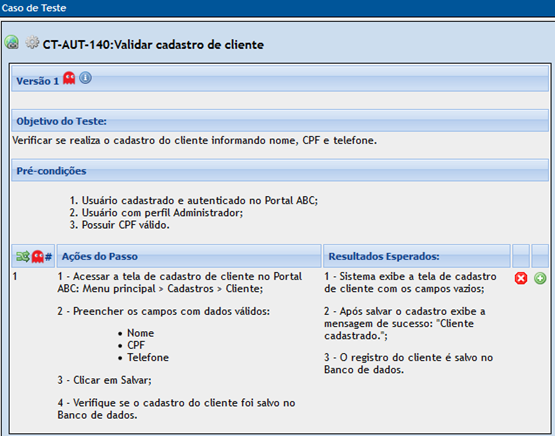
\includegraphics[scale=1.0]{imagens/ExcemplodeCasodeTeste.png}
	\\\textbf{Fonte:} Elaborada pelo autor
	\label{fig:exemploDeCasoDeTeste}
\end{figure}
\FloatBarrier
\input{capitulo09Implantacao}
\chapter{Resultados e Discussão}
\label{cap:resultados}

Este capítulo apresenta os resultados da avaliação de desempenho do motor de inferência,
conduzida segundo o protocolo descrito na Seção~\ref{sec:estrategia-testes}. Os resultados
são organizados nos dois regimes de execução previstos, o regime irrestrito e o regime de
seleção parcial, seguidos de uma análise comparativa que relaciona a evidência empírica
obtida às questões de pesquisa formuladas no Capítulo~\ref{cap:01}.

\section{Regime Irrestrito}
\label{sec:resultado-irrestrito}

No regime irrestrito, os domínios de todas as categorias permanecem completos, situação que
corresponde ao catálogo antes de qualquer seleção do usuário. A
Tabela~\ref{tab:bench-regime1} apresenta o desempenho dos dois motores para tamanhos de
domínio crescentes.

\begin{table}[htbp]
  \centering
  \caption{Desempenho dos motores no regime irrestrito}
  \label{tab:bench-regime1}
  \resizebox{\ifdim\width>\linewidth\linewidth\else\width\fi}{!}{%
    \begin{tabular}{rrrrrcr}
      \toprule
      $d$ & AC-3 checagens & AC-3 tempo (ms) & FB checagens         & FB tempo (ms) & FB concl. & Espaço residual       \\
      \midrule
      10  & 118            & 0,093           & 152000               & 5,586         & sim       & 100000                \\
      25  & 302            & 0,039           & $1{,}46\times10^{7}$ & 510,548       & sim       & $9{,}77\times10^{6}$  \\
      50  & 608            & 0,076           & $1{,}50\times10^{8}$ & 5183,057      & não       & $3{,}13\times10^{8}$  \\
      75  & 915            & 0,101           & $1{,}51\times10^{8}$ & 5191,575      & não       & $2{,}37\times10^{9}$  \\
      100 & 1225           & 0,128           & $1{,}50\times10^{8}$ & 5443,806      & não       & $1{,}00\times10^{10}$ \\
      250 & 3058           & 0,288           & $1{,}63\times10^{8}$ & 6014,267      & não       & $9{,}77\times10^{11}$ \\
      500 & 6125           & 0,637           & $2{,}26\times10^{8}$ & 10076,577     & não       & $3{,}13\times10^{13}$ \\
      \bottomrule
    \end{tabular}%
  }
  \fonte{Elaborada pelo autor}
\end{table}

Os dados evidenciam duas observações centrais. A primeira diz respeito à força bruta, cujo
custo cresce em conformidade com a natureza exponencial do produto cartesiano. A avaliação
exaustiva conclui apenas para os menores valores de $d$, atingindo o teto de aborto a partir
de $d=50$, quando o número de combinações a examinar ultrapassa a ordem de $10^8$. A partir
desse ponto, os valores registrados para a força bruta correspondem ao custo acumulado até a
interrupção, e não ao custo total que a avaliação demandaria, o qual cresceria até
$3{,}13\times10^{13}$ combinações em $d=500$.

A segunda observação diz respeito ao AC-3, que conclui em todos os valores de $d$ em tempo
inferior a um milissegundo, executando algumas milhares de avaliações de restrição mesmo no
maior cenário, com $6{,}125$ checagens em $d=500$. Observa-se, contudo, que o espaço residual
produzido pelo AC-3 permanece exatamente igual a $d^5$ em todos os casos, o que indica que a
arco-consistência não removeu nenhum valor dos domínios.

Essa ausência de poda não constitui ineficiência do motor, mas era prevista pela análise estrutural da Subseção 2.4.2. Com domínios completos sobre um grafo acíclico, cada valor de uma variável encontra suporte em ao menos um valor de cada variável vizinha, de modo que a rede já se apresenta arco-consistente e nenhum valor se torna elegível à remoção. O motor executa, verifica a consistência e encerra sem podar. A
Figura~\ref{fig:bench-checagens} ilustra esse contraste, no qual a curva da força bruta
acompanha a progressão teórica de $d^5$ até atingir o teto de aborto, ao passo que a curva do
AC-3 permanece praticamente constante em ordens de magnitude inferiores.

\begin{figure}[htb]
  \centering
  \caption{Número de avaliações de restrição em função do tamanho do domínio $d$}
  \label{fig:bench-checagens}
  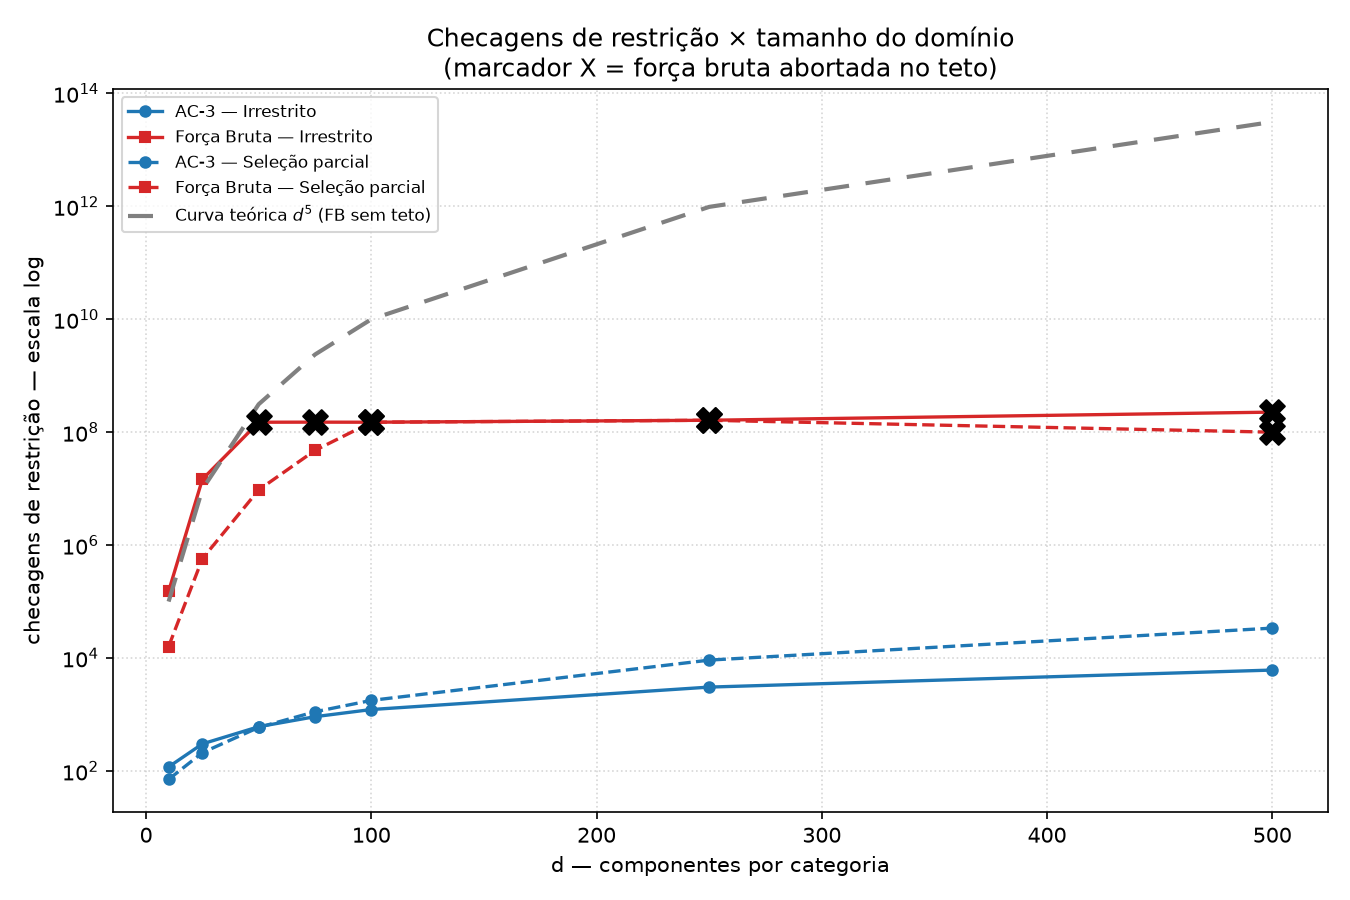
\includegraphics[width=0.85\textwidth]{imagens/output/fig_checagens.png}
  \fonte{Elaborada pelo autor}
\end{figure}

\section{Regime de Seleção Parcial}
\label{sec:resultado-selecao}

No regime de seleção parcial, uma das variáveis é fixada em um único valor, situação que
corresponde a uma etapa intermediária do wizard, na qual o usuário já selecionou um
componente. Para este experimento, fixou-se a categoria CPU em um processador de soquete AM5.
A Tabela~\ref{tab:bench-regime2} apresenta os resultados.

\begin{table}[htbp]
\centering
\caption{Desempenho dos motores no regime de seleção parcial}
\label{tab:bench-regime2}
\resizebox{\ifdim\width>\linewidth\linewidth\else\width\fi}{!}{%
\begin{tabular}{rrrrrcrr}
\toprule
$d$ & AC-3 checagens & AC-3 tempo (ms) & FB checagens & FB tempo (ms) & FB concl. & Residual & Redução ($d^5$/residual) \\
\midrule
10 & 71 & 0,038 & 16000 & 0,558 & sim & 1500 & $\times$67 \\
25 & 211 & 0,030 & 574375 & 21,256 & sim & 45000 & $\times$217 \\
50 & 591 & 0,055 & $9{,}50\times10^{6}$ & 344,182 & sim & 812500 & $\times$385 \\
75 & 1118 & 0,082 & $4{,}76\times10^{7}$ & 1711,388 & sim & $3{,}95\times10^{6}$ & $\times$600 \\
100 & 1778 & 0,217 & $1{,}50\times10^{8}$ & 5433,302 & não & $1{,}25\times10^{7}$ & $\times$800 \\
250 & 9191 & 0,294 & $1{,}63\times10^{8}$ & 6148,752 & não & $4{,}92\times10^{8}$ & $\times$1984 \\
500 & 33878 & 1,222 & $1{,}00\times10^{8}$ & 2830,519 & não & $7{,}81\times10^{9}$ & $\times$4000 \\
\bottomrule
\end{tabular}%
}
\fonte{Elaborada pelo autor}
\end{table}

Diferentemente do regime anterior, a arco-consistência agora produz poda efetiva. Ao fixar a
CPU em um único valor de soquete AM5, todas as placas-mãe de soquete distinto perdem seu
único suporte possível e são removidas do domínio. Essa remoção propaga-se de forma
transitiva à categoria RAM, uma vez que a eliminação das placas de soquete incompatível
elimina também o suporte aos módulos de memória de padrão correspondente. Como consequência,
o espaço residual cai muito abaixo de $d^5$, com uma redução que evolui de $\times67$ em
$d=10$ a $\times4000$ em $d=500$.

A composição do espaço residual explicita o mecanismo da poda. Para $d=50$, o residual de
$812{,}500$ configurações decompõe-se no produto entre a CPU fixada, as $13$ placas-mãe de
soquete AM5 remanescentes, os $25$ módulos de memória de padrão DDR5 remanescentes e as $50$
GPUs e $50$ fontes preservadas. As categorias GPU e Fonte não sofrem poda porque participam
apenas da restrição quantitativa de capacidade energética, não sendo afetadas pela seleção do
soquete da CPU. Esse comportamento reproduz precisamente o de um CSP dinâmico, no qual cada
decisão do usuário restringe o conjunto de valores admissíveis das variáveis relacionadas
\cite{Mittal1989}.

Cabe observar que, neste regime, o AC-3 executa um número maior de avaliações de restrição
que no regime irrestrito, alcançando $33{,}878$ checagens em $d=500$ contra $6{,}125$ no caso
irrestrito. Esse acréscimo decorre da própria propagação, pois cada remoção de valor implica
a reinserção dos arcos afetados na fila para reverificação. O custo adicional é, todavia,
desprezível em termos absolutos, mantendo-se em $1{,}222$ ms, e é largamente compensado pela
redução de ordens de magnitude no espaço de busca resultante.

\section{Análise Comparativa}
\label{sec:resultado-comparativo}

A Tabela~\ref{tab:bench-comparativa} confronta os dois regimes para um mesmo tamanho de
domínio, $d=50$, sintetizando as duas naturezas distintas de ganho observadas.

\begin{table}[htbp]
  \centering
  \caption{Comparação entre os regimes para $d = 50$}
  \label{tab:bench-comparativa}
  \begin{tabular}{lrr}
    \toprule
    Métrica                & Irrestrito           & Seleção parcial      \\
    \midrule
    Espaço residual (AC-3) & $3{,}13\times10^{8}$ & 812500               \\
    $d^5$ (teórico)        & $3{,}13\times10^{8}$ & $3{,}13\times10^{8}$ \\
    AC-3 checagens         & 608                  & 591                  \\
    AC-3 tempo (ms)        & 0,076                & 0,055                \\
    FB checagens           & $1{,}50\times10^{8}$ & $9{,}50\times10^{6}$ \\
    FB concl.              & não                  & sim                  \\
    FB config.\ válidas    & ---                  & 749125               \\
    \bottomrule
  \end{tabular}
  \fonte{Elaborada pelo autor}
\end{table}

A comparação evidencia que o motor de inferência oferece duas economias complementares. No
regime irrestrito, ainda que não haja poda, o AC-3 decide a consistência da rede com $608$
avaliações de restrição, ao passo que a força bruta não conclui a enumeração sequer dentro do
teto estabelecido. Trata-se de um ganho puramente algorítmico, decorrente de o motor não
necessitar percorrer o espaço de configurações completas. No regime de seleção parcial,
soma-se a esse ganho a poda propagada, que reduz o espaço residual de $3{,}13\times10^{8}$
para $812{,}500$ configurações. Nesse cenário, a força bruta passa a concluir a enumeração e
identifica $749{,}125$ configurações válidas, valor coerente com o espaço residual reportado
pelo AC-3, uma vez que este constitui um limite superior sobre o conjunto de soluções.

A Figura~\ref{fig:bench-tempo} apresenta o tempo de execução dos dois motores em ambos os
regimes, corroborando, sob a métrica temporal, o comportamento já observado sob a métrica de
avaliações de restrição.

\begin{figure}[htb]
  \centering
  \caption{Tempo de execução em função do tamanho do domínio $d$, por regime}
  \label{fig:bench-tempo}
  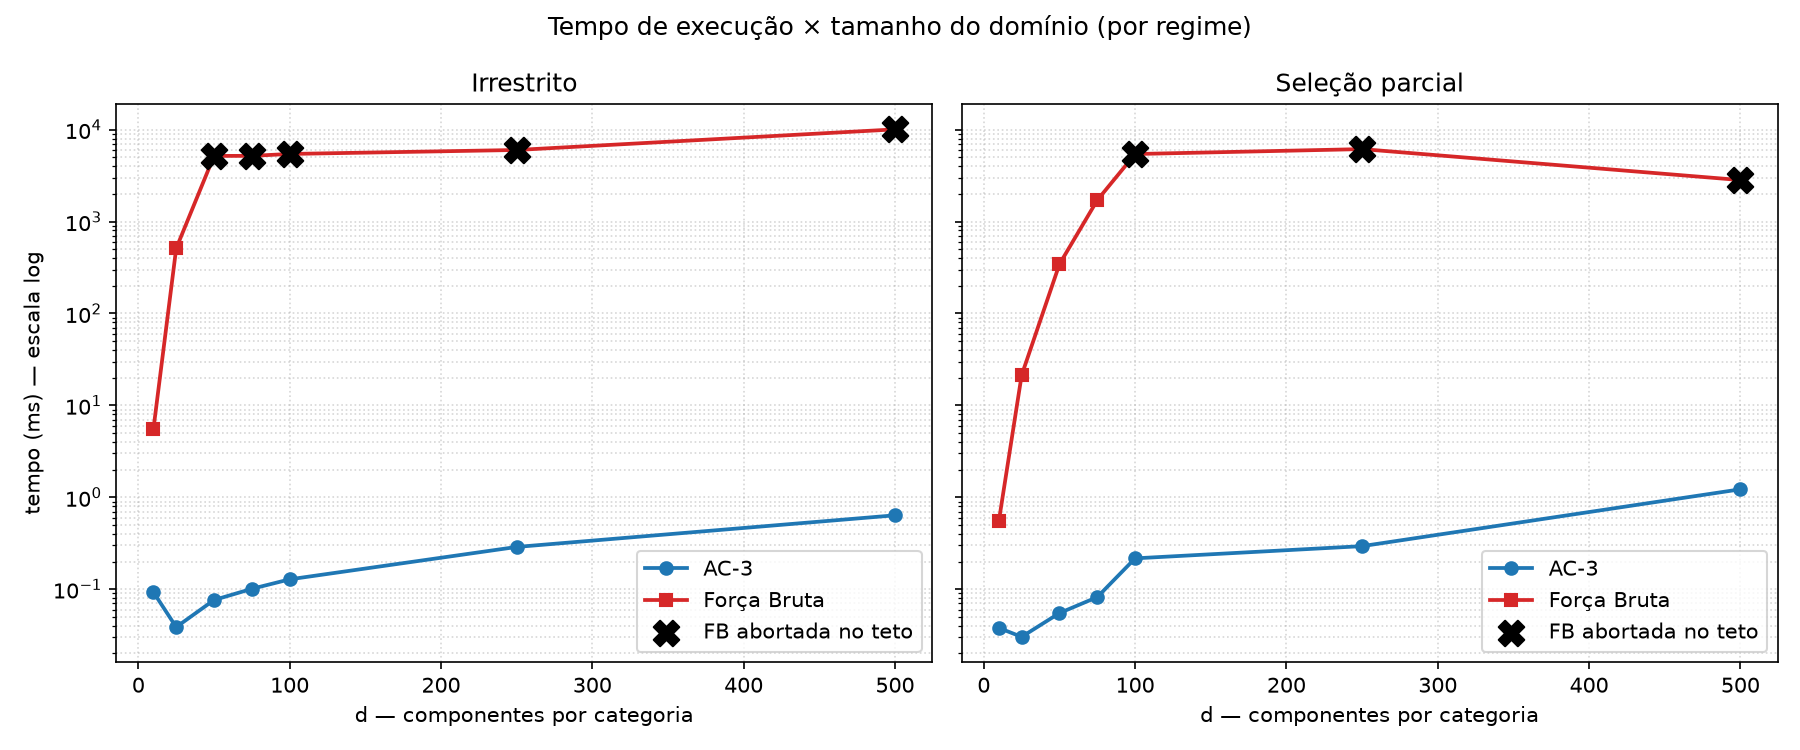
\includegraphics[width=0.85\textwidth]{imagens/output/fig_tempo.png}
  \fonte{Elaborada pelo autor}
\end{figure}

Os resultados sustentam empiricamente a resposta à questão de pesquisa de natureza técnica
formulada no Capítulo~\ref{cap:01}. A validação de configurações de hardware por meio de
propagação de restrições mostra-se viável em tempo praticamente constante e em ordens de
magnitude inferiores à avaliação exaustiva, cuja inviabilidade, decorrente da natureza
NP-completa do CSP, é confirmada pela impossibilidade de conclusão da força bruta a partir de
$d=50$. Confirma-se, ainda, que o efeito de redução de domínio característico da propagação de
restrições manifesta-se precisamente sob seleção parcial, situação que corresponde ao uso real
do sistema, no qual o usuário constrói sua configuração de forma incremental.
% \input{capitulo11TrabalhosRelacionados}
\chapter{Conclusões Parciais}
\label{cap:12}

Este trabalho propôs o desenvolvimento de um sistema especialista educacional para
validação de compatibilidade de \textit{hardware}, fundamentado no formalismo de Problemas de
Satisfação de Restrições e no algoritmo de propagação AC-3, com a finalidade de não apenas
detectar incompatibilidades entre componentes, mas de comunicar ao usuário leigo a razão
técnica de cada uma em linguagem acessível. Nesta etapa de Validação de Projeto,
apresentam-se as conclusões parciais obtidas a partir do que já foi elicitado, modelado e
implementado.

O objetivo geral mostrou-se plenamente viável ao longo do desenvolvimento. A modelagem do
problema de compatibilidade de \textit{hardware} como um CSP revelou-se adequada, uma vez que as
três categorias de restrições estudadas, soquete, padrão de memória e capacidade
energética, ajustaram-se naturalmente à estrutura de variáveis, domínios e restrições.
Sobre essa modelagem, o algoritmo AC-3 foi implementado como motor de inferência funcional,
capaz de propagar restrições de forma incremental e podar os domínios das variáveis a cada
seleção do usuário, sem recorrer à avaliação exaustiva por força bruta. Essa afirmação
deixou de ser apenas teórica: a avaliação de desempenho conduzida no
Capítulo~\ref{cap:resultados} comprovou empiricamente que a propagação de restrições decide
a consistência da rede em ordens de magnitude menos avaliações que a enumeração exaustiva,
a qual sequer conclui dentro do teto estabelecido a partir de domínios com cinquenta
componentes por categoria.

Quanto aos objetivos específicos, os resultados parciais são igualmente favoráveis. A
representação de conhecimento adotada, baseada em um modelo genérico de metadados, permitiu
dissociar o motor de inferência do domínio de aplicação, de modo que as regras de
compatibilidade residem inteiramente na base de conhecimento e não no código. Essa decisão
concretizou os requisitos de expansibilidade estabelecidos, pois a inclusão de novas
categorias, características ou restrições depende apenas da inserção de registros, sem
alteração do algoritmo. O mecanismo de explicação também foi implementado, gerando para
cada incompatibilidade uma justificativa em linguagem natural a partir de modelos de texto
associados às restrições, o que assegura que nenhum bloqueio ocorra de forma silenciosa.

A aplicação do motor ao domínio de compatibilidade de \textit{hardware}, tomado como estudo de caso,
confirmou a validade da abordagem. A base de conhecimento foi populada com componentes
reais das plataformas AM4 e AM5, e os cenários de teste demonstraram que o sistema
identifica corretamente as incompatibilidades de soquete, memória e potência, apresentando
as justificativas correspondentes. A interface no formato wizard, por sua vez, materializou
o caráter educativo da solução ao manter os componentes incompatíveis visíveis e
acompanhados de suas explicações, em vez de simplesmente ocultá-los.

Do ponto de vista do problema de pesquisa, os resultados parciais indicam que é possível
construir um sistema especialista que valide a compatibilidade de \textit{hardware} por meio de um
motor formal e que, ao mesmo tempo, ensine o usuário comunicando a razão de cada
incompatibilidade. A articulação entre a validação por propagação de restrições e a
capacidade de explicação herdada dos sistemas especialistas mostrou-se não apenas possível,
mas coerente, atendendo simultaneamente à dimensão técnica e à dimensão pedagógica que
motivaram o trabalho. A evidência experimental reforça essa conclusão sob dois regimes
complementares. Na ausência de seleção, a vantagem do motor é de natureza algorítmica, pois
a consistência é decidida sem enumerar o espaço de configurações completas. Sob seleção
parcial, situação que caracteriza o uso real do sistema, soma-se a esse ganho a redução
efetiva do espaço de busca por propagação, o que confirma a adequação da abordagem à
interação incremental do usuário com o wizard.

Reconhecem-se, contudo, as limitações próprias do estágio atual. A corretude das validações
depende do cadastro correto das restrições na base de conhecimento, característica inerente
aos sistemas dirigidos a dados. A validação da capacidade energética é realizada de forma
binária, componente a componente, preservando a natureza do grafo de restrições, ao passo
que o consumo agregado da configuração é apresentado apenas como informação. Além disso, a
estratégia de testes automatizados encontra-se parcialmente desenvolvida, com os testes de
integração e de interface previstos como atividade posterior.

Para a etapa de Avaliação Final, planeja-se a ampliação da base de conhecimento para
contemplar outras plataformas e categorias de componentes, a complementação da estratégia
de testes automatizados e a realização de uma avaliação da eficácia educativa da solução
junto a usuários. As conclusões parciais aqui apresentadas confirmam que os objetivos
propostos são alcançáveis e que o sistema desenvolvido cumpre, até o presente estágio, os
propósitos técnico e educacional que fundamentaram este trabalho.
\input{capitulo13Cronograma}






% ---------------------------------------------------------------------------------
%                                 ELEMENTOS PÓS-TEXTUAIS
% ---------------------------------------------------------------------------------
\postextual


% ----------------------------------------------------------
% Referências bibliográficas
% ----------------------------------------------------------
\printbibliography


% ----------------------------------------------------------
% Glossário
% ----------------------------------------------------------
%
% Consulte o manual da classe abntex2 para orientações sobre o glossário.
%
%\glossary


% ----------------------------------------------------------
% Apêndices
% ----------------------------------------------------------
% \input{pos01Apendices}


% ----------------------------------------------------------
% Anexos
% ----------------------------------------------------------
% \input{pos02Anexos}


%---------------------------------------------------------------------
% ÍNDICE REMISSIVO
%---------------------------------------------------------------------

%\phantompart

%\printindex


\end{document}
